\documentclass[11pt,reqno]{amsart}
\usepackage[T1]{fontenc}
\usepackage{lmodern}
\usepackage{amsmath,amssymb,amsthm,mathtools,bm}
\usepackage{enumitem}
\usepackage{graphicx}
\usepackage{xcolor}
\usepackage{tikz}
\usetikzlibrary{arrows.meta,positioning,calc,fit,patterns,decorations.pathreplacing}
\usepackage{microtype}
\usepackage[margin=1.12in]{geometry}
\usepackage[pdfencoding=auto,psdextra]{hyperref}
\usepackage[nameinlink,noabbrev,capitalise]{cleveref}
\hypersetup{
 colorlinks=true,
 linkcolor=blue!45!black,
 citecolor=green!35!black,
 urlcolor=blue!55!black,
 pdftitle={A uniform Hilbert transform estimate for Lipschitz directions},
 pdfauthor={OpenAI}
}
\numberwithin{equation}{section}
\newtheorem{theorem}{Theorem}[section]
\newtheorem{proposition}[theorem]{Proposition}
\newtheorem{lemma}[theorem]{Lemma}
\newtheorem{corollary}[theorem]{Corollary}
\theoremstyle{definition}
\newtheorem{definition}[theorem]{Definition}
\theoremstyle{remark}
\newtheorem{remark}[theorem]{Remark}
\newcommand{\R}{\mathbb R}
\newcommand{\C}{\mathbb C}
\newcommand{\N}{\mathbb N}
\newcommand{\Z}{\mathbb Z}
\newcommand{\E}{\mathbb E}
\newcommand{\dd}{\,\mathrm d}
\newcommand{\one}{\mathbf 1}
\DeclareMathOperator{\Lip}{Lip}
\DeclareMathOperator{\supp}{supp}
\DeclareMathOperator{\dist}{dist}
\newcommand{\norm}[1]{\left\|#1\right\|}
\newcommand{\abs}[1]{\left|#1\right|}
\allowdisplaybreaks[2]
\setlist[enumerate]{itemsep=3pt,topsep=5pt}
\setlist[itemize]{itemsep=3pt,topsep=5pt}
\emergencystretch=1em

\title[Hilbert transforms along Lipschitz directions]{A uniform Hilbert transform estimate for Lipschitz directions}
\author{OpenAI}
\date{September 25, 2026}
\begin{document}
\begin{abstract}
We prove a uniform \(L^2\) bound for the Hilbert transform along a
Lipschitz unit vector field in the plane, with integration restricted
to a fixed absolute multiple of the reciprocal Lipschitz seminorm.
The bound is uniform in the inner truncation and holds for fields
depending on both coordinates. This gives an affirmative answer to
Stein's weak-\((2,2)\) conjecture.
\end{abstract}
\maketitle
\tableofcontents
\clearpage
\section{Short transforms and band reduction}
\label{intro:section}

Let \(v:\R^2\to S^1\) be a Lipschitz unit vector field. For
\(0<\epsilon<a\), define the short directional Hilbert transform by
\[
 H_{v,a}^{\epsilon}f(x)
 =\int_{\epsilon<|t|<a}f(x-tv(x))\,\frac{\mathrm dt}{t}.
\]
The direction is held fixed at the output point \(x\): the integral
samples the straight line through \(x\) in direction \(v(x)\).
For \(f\in\mathcal S(\R^2)\), the symmetric principal value
\(H_{v,a}f=\lim_{\epsilon\downarrow0}H_{v,a}^{\epsilon}f\)
exists at every point, since
\(f(x-tv(x))-f(x+tv(x))=O_x(|t|)\) near zero.

\begin{theorem}\label{thm:main}
There are absolute constants \(a_*\in(0,1/2)\) and \(C_*<\infty\)
such that every Lipschitz field \(v:\R^2\to S^1\) with
\(\Lip(v)\le1\) satisfies
\[
 \sup_{0<\epsilon<a_*}
 \norm{H_{v,a_*}^{\epsilon}f}_{L^2(\R^2)}
 \le C_*\norm{f}_{L^2(\R^2)}
 \qquad(f\in\mathcal S(\R^2)).
\]
Its symmetric principal value therefore satisfies
\[
 \norm{H_{v,a_*}f}_2\le C_*\norm f_2,
 \qquad
 \big|\{x:|H_{v,a_*}f(x)|>\lambda\}\big|
 \le C_*^2\lambda^{-2}\norm f_2^2
 \quad(\lambda>0).
\]
\end{theorem}

Both coordinates may enter the field arbitrarily subject to the
Lipschitz bound. The supremum in the theorem is outside the norm,
so its first assertion is a uniform operator bound for each inner
truncation. The principal-value assertion is stated on Schwartz
functions and gives an \(L^2\)-bounded extension by density.

The outer length has a natural scaling. If \(L_v=\Lip(v)>0\), put
\(\widetilde v(X)=v(X/L_v)\) and
\(\widetilde f(X)=f(X/L_v)\). Then \(\Lip(\widetilde v)=1\), and
changing variables \(s=L_vt\) gives
\[
 H_{v,a_*/L_v}^{\epsilon}f(x)
 =H_{\widetilde v,a_*}^{L_v\epsilon}\widetilde f(L_vx),
 \qquad \norm{\widetilde f}_2=L_v\norm f_2.
\]
The theorem thus has the same constant at outer length \(a_*/L_v\).
If \(L_v=0\), the field is constant. Rotation and Fubini reduce its
transform, for any finite outer length, to the one-dimensional
Hilbert transform. These conventions distinguish the short-scale
assertion from an estimate at arbitrary outer lengths for varying
fields.

\subsection{The problem and its predecessors}

Stein's question places Lipschitz regularity at the center of the
planar directional singular-integral problem. In the formulation
\cite[Conjecture~1.5]{LLStein}, it asks for a uniform weak-\((2,2)\)
bound with the outer length controlled by the reciprocal Lipschitz
seminorm. \Cref{thm:main} gives an affirmative answer with a strong
\(L^2\) bound. The scale restriction limits the turning of the field,
but it does not make the operator a Fourier multiplier: the line
used by the integral still varies with the output point.

Lacey and Li trace Stein's question to Zygmund's conjecture on
almost-everywhere differentiation by averages over shrinking straight
segments in direction \(v(x)\). They also recall a Besicovitch
obstruction showing that H\"older regularity of any exponent below one
does not by itself give the corresponding uniform weak-\((2,2)\)
estimate for the short positive averaging maximal operator
\cite[Preface, Conjecture~1.2 and Chapter~2]{LLStein}.
Analytic fields admit additional structure:
Bourgain proved an \(L^2\) theorem for their averaging maximal
operator \cite{Bourgain1989}, and Stein and Street proved local
\(L^p\), \(1<p<\infty\), estimates for single-parameter singular
Radon transforms associated with real-analytic maps
\cite{SteinStreet2012}. Their
singular-integral theorem includes analytic frozen-direction Hilbert
transforms, with localization depending on the analytic map. The
uniform Lipschitz estimate considered here asks for constants
controlled by the Lipschitz seminorm alone.

Several distinct advances explain the remaining difficulty. Lacey
and Li proved an annular weak-\((2,2)\) estimate, together with strong
\(L^p\) estimates for \(p>2\), for directional Hilbert transforms
with measurable directions \cite[Theorem~1.1]{LLAnnular}. An annular
restriction isolates a frequency scale; it does not give a uniform
strong \(L^2\) bound for the complete transform. For Lipschitz unit
fields, Guo obtained annular weak-\((2,2)\) and strong \(L^p\),
\(p>2\), bounds, uniformly in the annulus scale, for the
\(r\)-variation, \(r>2\), of
smooth dyadic Hilbert-transform partial sums over the short scale range
determined by the reciprocal Lipschitz length; the varying dyadic
cutoff is distinct from the hard inner time cutoff in \Cref{thm:main}
\cite[Theorem~1.2 and (1.6)--(1.8) of the author version]{GuoVariation2017}.
Lacey and Li's Lipschitz Kakeya theorem controls averages over short
rectangles on which the field has a prescribed popular direction
\cite[Theorem~1.4]{LLKakeya}.
For popularity \(\delta\), its weak-\(L^2\) norm costs
\(C\delta^{-1/2}\). We use precisely this estimate.

The Lacey--Li memoir develops the relation between those maximal
operators and the Hilbert-transform problem \cite{LLStein}. Its
Theorem~1.18 assumes a stronger maximal estimate below \(L^2\) for
the strong annular conclusion; its full-transform conclusion also
requires \(C^{1+\eta}\) regularity. These are conditional results with
hypotheses different from those of \Cref{thm:main}. For bounded
measurable slopes depending on one coordinate, Bateman proved
single-annulus \(L^p\) estimates for \(1<p<\infty\)
\cite{Bateman2013}. Bateman and Thiele proved strong \(L^p\) bounds
for the full-line principal-value transform when \(3/2<p<\infty\),
for every nonvanishing measurable field depending on one coordinate
\cite[Theorem~1]{BatemanThiele2013}. The one-coordinate \(L^2\) case is already connected to
Carleson's theorem by a partial Fourier transform
\cite{Carleson1966,BatemanThiele2013}; Bateman and Thiele obtain the stated wider
\(p\)-range. The one-coordinate hypothesis remains a substantive
restriction on the direction field. Guo extended the one-coordinate setting to
fields constant along suitable Lipschitz foliations, with a uniform
transversality assumption \cite{Guo2015,Guo2017}.

A different family of results combines Lipschitz control with
lacunary directions. Guo and Thiele proved strong \(L^p\) bounds
without a frequency restriction for short principal-value transforms
associated with dyadic roundings of a positive Lipschitz slope
\cite{GuoThiele2017}; Di Plinio and Parissis extended this framework
to finite lacunary order for fields generated by separated dyadic
roundings of Lipschitz angular functions \cite{DiPlinioParissis2018}.
The rounded direction field can itself be discontinuous. These
results exploit directional structure beyond that assumed in the
present theorem.

A further reduction separates frequency reassembly from the main
single-band estimate. Di Plinio, Guo, Thiele and Zorin-Kranich
established that uniform strong \(L^2\) bounds on vertical frequency
bands imply the full short principal-value bound under a small uniform
Lipschitz bound in the vertical variable
\cite[Corollaries~1.3--1.4 of the author version]{DiPlinioGuoThieleZorinKranich2018}.
We give a commutator proof adapted to the two truncation endpoints
and to the narrow frequency bins used later. The new estimate to be
proved is the logarithmically improved restricted bound on a band;
the principle of band-to-full reassembly is already present in that
work.

\subsection{The analytic and geometric reductions}

We describe the proof before fixing its technical parameters.
Localization and rotation write a short piece of the operator in
slope form
\[
 H_{u,a}^{\epsilon}h(x,y)
 =\int_{\epsilon<|t|<a}
 h(x-t,y-tu(x,y))\,\frac{\mathrm dt}{t},
 \qquad |u|\le1,\quad \Lip(u)\le C,
\]
with both input and test supported in a short horizontal strip.
Writing \(\eta\) for the frequency dual to \(y\), a vertical
frequency band at scale \(w\) means that \(|\eta|\) is comparable
to \(w^{-1}\). For its smooth projection \(P_w\), the
central restricted estimate is
\[
 |\langle H_{u,a}^{\epsilon}P_w f,g\rangle|
 \lesssim
 \bigl(1+|\log(|F|/|E|)|\bigr)^{-3}\sqrt{|F||E|},
 \qquad |f|\le\one_F,\quad |g|\le\one_E.
\]
Here \(F,E\) are sets of positive finite measure in the horizontal
strip. Its constants are uniform in \(w\) and \(\epsilon\). The logarithmic
factor makes amplitude-level summation converge. A Lipschitz
commutator then permits Littlewood--Paley reassembly across vertical
bands. These implications, including all endpoint errors, are proved
in this section before the restricted estimate itself is used.

The difficult regime is \(|E|\gg|F|\). Write
\(L=\log\sqrt{|E|/|F|}\). Positive operator bounds discard all but
very short integration times. The vertical band is then divided into
narrow intervals centered at frequencies \(\eta_j\), with common
width comparable to \(W^{-1}\), where \(W=mw\) and \(m\) grows
subexponentially in \(L\). The components form one finite-dimensional
Hilbert space. A wave packet has horizontal length \(\ell\),
transverse width \(W\), and a direction label with precision
\(d=w/\ell\). Smooth packet forms retain the original field only
through scalar selectors of its direction.

Ordinary size and density estimates remove the small-density packets.
Each remaining packet is assigned to a top box whose direction is
popular on a measured subset of the test set. The popularity witnesses
are disjoint. Lacey--Li's theorem controls a decaying weighted count
of the tops, after every thin parallelogram has been enclosed by an
admissible orthogonal rectangle. This step is geometric: it supplies
a polynomial cost in \(L\), and does not provide the final
oscillatory saving.

\subsection{The phase gain and its iteration}

Two statements make the oscillation usable. First, on every reference
line the packet sums have polynomial moment bounds, square-function
bounds and \(3\)-variation bounds. The variation argument combines
L\'epingle's martingale inequality with the comparison between
smooth Fourier truncations and conditional expectations developed
by Jones, Seeger and Wright \cite{Lepingle1976,JSW2008}. All three
packet estimates hold for every fixed deterministic subcollection. Popularity and Lipschitz control then
produce one exceptional set outside which each separated list of
significant top directions in the required angular cluster and
precision range has at most \(D=L^C\) members, simultaneously over
angular resolutions.

Second, a finite Fourier sum with at most \(D\) separated real
frequencies has a strict improvement over the usual coefficient
exponent. For suitable band-limited probability measures \(\nu\),
we prove
\[
 \left\|\sum_{i=1}^d a_i e^{i\lambda_i t}\right\|_{L^p(\nu)}
 \le \left(\sum_{i=1}^d |a_i|^{r_*}\right)^{1/r_*},
 \qquad
 \frac1{r_*}=1-\frac{1+c/\log(2D)}p,
 \quad p\ge4.
\]
The operator constant is exactly one, for complex coefficients and
for Hilbert-valued coefficients acted on by diagonal phases.
The proof separates the case of one dominant coefficient from its
complement. In the latter case, separated quantiles give a strict
fourth-moment deficit, which survives a small improvement of the
coefficient exponent. An unspecified constant in this inequality
would accumulate at every angular level and destroy the argument.

The iteration organizes directions into nested angular intervals.
Each interval carries the positive mass of the tops whose direction
precision is sufficiently fine for that interval; these are its
eligible tops. It also carries an oscillatory amplitude assembled
from its packets. The significant-direction count enters phase
averaging through a weighted selection of separated block children,
whose analytic weights cancel the probability cost of retaining them.
We compare mass-normalized \(p\)-energies after adding the mass itself
as a baseline. On an appropriate spatial interval, a finer amplitude
can be predicted from one good point by diagonal phase motion. The
finite Fourier estimate therefore controls the average of the
predicted energy factor. The comparison errors are proportional to the
relative mass lost on the path, so their sum is controlled by a
logarithmic mass telescope.

Packets that stop between two angular endpoints create residual
terms. Square summation handles blocks with a definite mass drop.
Across nearly unary portions of a path, the energies telescope and
the remaining residual sums are estimated by \(3\)-variation of
one fixed sequence for that path. The sequence is chosen before the
spatial point or mass stop is selected. Normalized factors on nested
spatial cells can then be integrated without any cost proportional
to the angular depth.

Finally we interpolate among shifted groupings of angular levels.
At the central parameter the packet coefficients contain boundary
weights. Averaging one common angular-grid translation removes these
weights, using eligibility as well as angular proximity in the
boundary telescope. With \(p=L^{1/2}\), the strict phase gain leaves
a decrease of order \((\sqrt L\log L)^{-1}\) in the exponent of
\(\sqrt{|E|/|F|}\). This dominates all fixed polynomial losses and
supplies the logarithmic restricted estimate above.

\subsection{Organization, inputs and uniformity}

Section~\ref{intro:section} gives the analytic reduction and the
precise packet estimates needed for the band theorem.
Section~\ref{tile:section} proves the ordinary tile estimates and
constructs the popular forest.
Section~\ref{conc:section} establishes every-line concentration and
the simultaneous count of significant directions.
Section~\ref{phase:section} proves the constant-one finite Fourier
inequality.
Section~\ref{hier:section} constructs the angular hierarchy and the
predicted factors.
Section~\ref{res:section} controls residuals and integrates path
products.
Section~\ref{assembly:section} performs interpolation, angular-grid
averaging and the final strong-type assembly.

There are two specialized external inputs: Lacey--Li's short
Lipschitz-popularity maximal theorem, stated in
\Cref{red:kakeya}, and the unweighted scalar martingale
\(3\)-variation inequality of L\'epingle, used in the form
\cite[Theorem~1.1, \(p=2\), \(r=3\), weight one]{ZorinKranich2020}.
The latter enters the locally proved Fourier/martingale comparison
in \Cref{conc:annular-variation}; we credit its origin to
\cite{Lepingle1976}. Standard one-dimensional Hilbert-transform,
maximal-function and interpolation facts are recalled where used.
The commutator, tile, concentration, finite-phase and hierarchy
arguments are included in full.

All packet collections, scale ranges and angular depths are finite
until estimates independent of those truncations have been proved.
The bin Hilbert spaces are finite-dimensional and complex, and every
constant is independent of their dimension. Pairings are linear in
the first variable. A factor \(L^C\) always has a fixed exponent;
it never conceals the number of packets, scales or hierarchy levels.

\subsection{Fourier conventions and the local reduction}
\label{red:section}

We use the Fourier convention
\[
 \widehat f(\xi,\eta)
   =\int_{\R^2}f(x,y)e^{-i(x\xi+y\eta)}\dd x\dd y,
 \qquad
 f(x,y)=\frac1{(2\pi)^2}\int_{\R^2}
       \widehat f(\xi,\eta)e^{i(x\xi+y\eta)}\dd\xi\dd\eta.
\]
The same convention is used in one dimension. Pairings are linear in
the first entry. A constant depending on a fixed finite list of smooth
cutoffs or on their prescribed seminorms is an absolute constant.
No such list will depend on a frequency scale, an inner truncation,
the number of packets, or the dimension of the bin Hilbert space.

\subsection{A maximal theorem and elementary analytic tools}

We first record precisely the specialized maximal theorem used later.
If an orthogonal rectangle \(R\) has long side \(L(R)\), short side
\(W(R)\), and long-side direction \(e_R\in S^1\), let
\(\operatorname{EX}(R)\) be the arc centered at \(e_R\) of total
length \(W(R)/L(R)\).

\begin{theorem}[Lacey--Li]\label{red:kakeya}
Let \(v:\R^2\to S^1\) be Lipschitz and \(0<\delta<1\). Restrict to
rectangles satisfying
\[
 L(R)\le \frac1{100\Lip(v)},\qquad
 \abs{R\cap v^{-1}(\operatorname{EX}(R))}\ge\delta\abs R,
\]
where the first restriction is void when \(\Lip(v)=0\). Then
\[
 \mathcal M_{v,\delta}h(z)
   =\sup_R\frac{\one_R(z)}{\abs R}\int_R\abs h
 \quad\text{satisfies}\quad
 \norm{\mathcal M_{v,\delta}h}_{L^{2,\infty}}
       \le C\delta^{-1/2}\norm h_2.
\]
Here the supremum is tested at every point of \(R\), and the constant
is independent of \(v\) and \(\delta\).
\end{theorem}

This is \cite[Theorem~1.4]{LLKakeya}. Requiring the field to lie in a
smaller fixed subarc only restricts the collection of admissible
rectangles. In the bounded slope range, the map
\(t\mapsto(1,t)/\sqrt{1+t^2}\) changes slope distances into arc
distances by comparable absolute factors. These observations explain
the slope version of \Cref{red:kakeya} used below. When an intermediate
box is a parallelogram, the application of the theorem will explicitly
enclose it by a comparable orthogonal rectangle of admissible length.

We also use the following familiar one-dimensional estimates, with
their indicated uniformities. The Hardy--Littlewood maximal operator
is bounded on \(L^p\), \(1<p<\infty\), and
\begin{equation}\label{red:horizontal-hilbert}
 \sup_{0<r<R<\infty}
 \left\|\int_{r<|t|<R}h(\,\cdot-t\,)\frac{\dd t}{t}\right\|_p
   \le C_p\norm h_p.
\end{equation}
The supremum in \eqref{red:horizontal-hilbert} is outside the norm;
the usual maximal truncation theorem gives this assertion as well.
See \cite[Theorems~1.1 and~7.6 and the proof of (7.7)]{Hajlasz2012}.
Fubini gives the corresponding horizontal estimates on \(\R^2\).
The \(L^2\) square-function identities used here are consequences of
Plancherel and finite overlap of smooth frequency annuli. The standard
smooth Littlewood--Paley and random-sign multiplier formulations are
also recorded in \cite[Proposition~5.3, Corollary~5.4, and
Remark~4.5]{Tao2006Notes4}. We give the particular Carleson embedding
and commutator arguments needed for our reduction below. The
John--Nirenberg and martingale variation estimates are stated in the
sections where their local forms are used.

\subsection{The local slope operator and its endpoints}

Fix an absolute bound \(C_{\rm Lip}\) large enough for the slope
fields obtained in the following localization; for example, a bound
of ten suffices after taking the squares small enough. Choose an
absolute horizontal length \(b_0>0\) with
\(b_0 C_{\rm Lip}<1/10\), and subsequently choose
\(0<a_*<b_0/100\). These constants may be decreased to accommodate
the fixed geometric enlargements in later applications of
\Cref{red:kakeya}. All such enlargements are chosen absolutely.
For the remainder of the local argument write \(a=a_*\), and put
\begin{equation}\label{red:local-operator}
 H_{u,a}^{\epsilon}h(x,y)
   =\int_{\epsilon<|t|<a}
      h(x-t,y-tu(x,y))\frac{\dd t}{t},
 \qquad 0<\epsilon<a,
\end{equation}
where \(\abs u\le1\) and \(\Lip(u)\le C_{\rm Lip}\).
The local inputs and tests will be supported in
\(I\times\R\), where \(I\) is any interval of length at most
\(b_0\).

\begin{lemma}\label{red:fixed-time}
For \(\abs t\,C_{\rm Lip}<1\), define
\[
 A_t h(x,y)=h(x-t,y-tu(x,y)).
\]
For \(1\le p<\infty\),
\begin{equation}\label{red:translate-bound}
 \norm{A_t h}_p
   \le (1-\abs t\,C_{\rm Lip})^{-1/p}\norm h_p,
\end{equation}
and \(A_t\) is a contraction on \(L^\infty\).
Consequently, replacing either symmetric endpoint at scale \(r\)
by a measurable endpoint between \(c r\) and \(C r\), with
\(c,C>0\) fixed and \(\max(1,C)r C_{\rm Lip}<1/2\), costs a bounded
\(L^p\) operator, independently of \(r\).
\end{lemma}

\begin{proof}
For each fixed \(x\), the map
\(\varphi_{x,t}(y)=y-tu(x,y)\) is increasing, onto, and satisfies
\[
 (1-\abs t\,C_{\rm Lip})\abs{y-y'}
 \le\abs{\varphi_{x,t}(y)-\varphi_{x,t}(y')}
 \le(1+\abs t\,C_{\rm Lip})\abs{y-y'}.
\]
The change-of-variables formula for a one-dimensional bi-Lipschitz
map, followed by translation in \(x\), proves
\eqref{red:translate-bound}. A difference of endpoint truncations
is pointwise dominated by
\[
 \int_{c' r<|t|<C' r}\abs{A_t h}\frac{\dd t}{|t|}
\]
with \(c'=\min(1,c)\) and \(C'=\max(1,C)\). Minkowski and
\eqref{red:translate-bound} bound this by
\(C_p\log(C'/c')\norm h_p\). The same proof applies to inner
and outer endpoints, and permits endpoints depending on \((x,y)\).
\end{proof}

We explain the localization of the original unit-field operator.
Partition the plane into squares \(Q\) of a sufficiently small fixed
side length. For output in \(Q\), only a fixed enlargement \(Q^+\)
of that square contributes to a transform of length \(a_*\). Rotate
coordinates so that the vector at the center of \(Q\) points along
the positive first coordinate axis. Since \(\Lip(v)\le1\), on the
rotated output square we have
\[
 v=(v_1,v_2),\qquad v_1\ge c>0,
 \qquad u=v_2/v_1,\qquad \abs u\le1,
 \qquad\Lip(u)\le C_{\rm Lip}.
\]
The last inequality follows by subtracting the two ratios and using
the lower bound for \(v_1\). Extend \(u\) to the plane with the
same Lipschitz bound, using
\(\inf_{z\in Q}(u(z)+C_{\rm Lip}|\,\cdot-z|)\), and then clip
the extension to \([-1,1]\). The infimum extension agrees with
\(u\) on \(Q\), and clipping preserves both agreement and the
Lipschitz bound.

At an output point, the substitution \(s=t v_1(x,y)\) changes
\(\dd t/t\) to \(\dd s/s\) and changes the two endpoints to
\(\epsilon v_1(x,y)\) and \(a_*v_1(x,y)\). By
\Cref{red:fixed-time}, each endpoint can be replaced by
\(\epsilon\) or \(a_*\), respectively, at a uniform \(L^2\)
cost. The rotated sets \(Q\) and \(Q^+\) fit in a common
horizontal interval of length at most \(b_0\), after choosing the
square side and \(a_*\) in that order. Thus a uniform bound for
\(\one_{I\times\R}H_{u,a}^{\epsilon}\one_{I\times\R}\)
implies the required bound on this output square. The output squares
are disjoint, the sets \(Q^+\) have bounded overlap, and rotations
preserve area. Squaring the local estimates and summing over \(Q\)
therefore proves the global estimate. Notice that both endpoint
errors are uniform in the inner radius \(\epsilon\).

\subsection{The band theorem and summation of amplitude levels}

A vertical band cutoff at length \(w>0\) is a multiplier
\(P_w=p(wD_y)\), where \(p\) is smooth and supported in a fixed
compact annulus
\(\{r:c_\eta\le|r|\le C_\eta\}\), with
\(0<c_\eta<C_\eta<\infty\) absolute. We allow a fixed bounded
family of such cutoffs, including slightly enlarged cutoffs equal to
one on the supports of others. All constants below are uniform when
the required finitely many cutoff seminorms are bounded. The dyadic
inverse frequency scale \(w\) belongs to \(2^{\Z}\).

\begin{theorem}[Restricted estimate on a vertical band]
\label{thm:band-restricted}
For the fixed absolute constants in \eqref{red:local-operator}, there
is an absolute \(C\) such that, for every field \(u\) with
\(\abs u\le1\) and \(\Lip(u)\le C_{\rm Lip}\), every
\(0<\epsilon<a\), every dyadic \(w\), and every vertical band
cutoff \(P_w\),
\begin{equation}\label{eq:src-1}
 \abs{\langle H_{u,a}^{\epsilon}P_w f,g\rangle}
 \le C\bigl(1+\abs{\log(|F|/|E|)}\bigr)^{-3}
       \sqrt{|F||E|}
\end{equation}
whenever \(F,E\subset I\times\R\) have positive finite measure,
\(\abs f\le\one_F\), \(\abs g\le\one_E\), and
\(\abs I\le b_0\).
\end{theorem}

The proof of \Cref{thm:band-restricted} will be completed after the
packet estimates and their iteration have been established. The next
results show, without using that theorem as a premise elsewhere in
its proof, that it implies \Cref{thm:main}. The last part of this
section then gives explicit sufficient packet estimates for
\Cref{thm:band-restricted}.

\begin{lemma}\label{red:restricted-strong}
Suppose a bilinear form \(\mathcal B\) satisfies
\[
 \abs{\mathcal B(f,g)}
 \le C_0(1+|\log(|F|/|E|)|)^{-3}\sqrt{|F||E|}
 \quad (|f|\le\one_F,\ |g|\le\one_E)
\]
on finite-measure sets in a fixed measurable domain. Then
\[
 \abs{\mathcal B(f,g)}\le C C_0\norm f_2\norm g_2
\]
for finite amplitude decompositions, and hence for all \(L^2\)
inputs whenever the form is obtained by an \(L^2\)-continuous
truncation or by completion from those inputs.
\end{lemma}

\begin{proof}
Use disjoint amplitude sets
\(F_i=\{2^{i-1}<|f|\le2^i\}\) and write
\(f=\sum_i2^i f_i\), where \(|f_i|\le\one_{F_i}\).
For the moment all sums are finite. Put
\(a_i=2^i\sqrt{|F_i|}\), so
\(\sum_i a_i^2\le4\norm f_2^2\).
Group the indices into measure classes
\[
 \mathcal I_k=\{i:2^k\le|F_i|<2^{k+1}\},\qquad
 A_k=\left(\sum_{i\in\mathcal I_k}a_i^2\right)^{1/2}.
\]
If \(i_0\) is the largest index in a nonempty class, then
\[
 \sum_{i\in\mathcal I_k}a_i
 \le 2^{(k+1)/2}\sum_{i\le i_0}2^i
 \le 2\sqrt2\,a_{i_0}\le2\sqrt2\,A_k.
\]
Make the analogous decomposition \(g=\sum_j2^j g_j\), with
measure classes \(\mathcal J_l\) and square sums \(B_l\).
For \(i\in\mathcal I_k\), \(j\in\mathcal J_l\),
\[
 (1+|\log(|F_i|/|E_j|)|)^{-3}
       \le C(1+|k-l|)^{-3}.
\]
The assumed bound, followed by the within-class estimates, gives
\[
 \abs{\mathcal B(f,g)}
   \le C C_0\sum_{k,l}(1+|k-l|)^{-3}A_kB_l
   \le C C_0\norm A_{\ell^2}\norm B_{\ell^2}.
\]
The final step is Young's inequality for the summable sequence
\((1+|k|)^{-3}\). This proves the assertion. Truncating the amplitude
decompositions and using the asserted continuity or completion gives
the last statement, with no dependence on the number of classes.
\end{proof}

\subsection{A Lipschitz commutator}

The estimate below belongs to the Lipschitz commutator theory initiated
by Calder\'on and developed by Coifman and Meyer
\cite{Calderon1965,CoifmanMeyer1978}. We give a dyadic proof with the
precise multiplier seminorms needed for Littlewood--Paley reassembly
and for the later narrow-bin reduction. The argument separates low
output frequencies from the annular interactions, because the constant
must remain uniform as the number of frequency scales increases.
Let \(\chi\) be a real even smooth cutoff equal to one on
\([-1,1]\) and supported in \([-2,2]\), and define
\[
 S_k=\chi(2^{-k}D),\qquad \Delta_k=S_k-S_{k-1}.
\]
Thus \(\Delta_k\) is supported in
\(\{2^{k-1}\le|\zeta|\le2^{k+1}\}\), and Plancherel gives
\begin{equation}\label{red:lp-square}
 \norm h_2^2\asymp\sum_k\norm{\Delta_kh}_2^2.
\end{equation}

\begin{lemma}[The required Carleson embedding]\label{red:carleson}
For every fixed integer \(c\), every \(q\in L^\infty(\R)\), and
every \(h\in L^2(\R)\),
\begin{equation}\label{red:carleson-estimate}
 \sum_k\norm{(\Delta_kq)S_{k+c}h}_2^2
      \le C_c\norm q_\infty^2\norm h_2^2.
\end{equation}
\end{lemma}

\begin{proof}
For a dyadic interval \(J\) of length \(2^{-j}\), split
\(q=q\one_{3J}+q\one_{(3J)^c}\). By
\eqref{red:lp-square}, the first part satisfies
\[
 \sum_{k\ge j}\int_J
       |\Delta_k(q\one_{3J})|^2
       \le C\norm q_\infty^2|J|.
\]
The kernels of \(\Delta_k\) have Schwartz decay at scale
\(2^{-k}\). For \(x\in J\) and \(k\ge j\), this gives
\[
 |\Delta_k(q\one_{(3J)^c})(x)|
     \le C\norm q_\infty 2^{j-k}.
\]
After summing the squares, we obtain
\begin{equation}\label{red:carleson-measure}
 \sum_{k\ge j}\int_J|\Delta_kq|^2
          \le C\norm q_\infty^2|J|.
\end{equation}
For each dyadic interval \(I\) of length \(2^{-k}\), set
\(\alpha_I=\int_I|\Delta_kq|^2\). Then
\eqref{red:carleson-measure} says
\(\sum_{I\subset J}\alpha_I\le C\norm q_\infty^2|J|\).

Write \(M\) for the Hardy--Littlewood maximal operator. Kernel
decay, summed on dyadic annuli about a point of \(I\), gives
\[
 \sup_{x\in I}|S_{k+c}h(x)|
       \le C_c\operatorname*{ess\,inf}_{y\in I}Mh(y).
\]
The shift \(c\) is fixed, so moving the kernel center across \(I\)
changes the bound by only a fixed factor. If \(F\ge0\) belongs to
\(L^2\), the dyadic Carleson condition implies
\[
 \sum_I\alpha_I
     \bigl(\operatorname*{ess\,inf}_I F\bigr)^2
       \le C\norm q_\infty^2\norm F_2^2.
\]
Indeed, for each \(t>0\), sum over the maximal dyadic intervals
on which \(\operatorname*{ess\,inf}_I F>t\), apply the Carleson
condition on each such interval, and integrate against \(2t\dd t\).
Their union lies, up to null sets, in \(\{F>t\}\).
Apply this assertion with \(F=Mh\), and use the \(L^2\) maximal
theorem. This proves \eqref{red:carleson-estimate}. This is also the
usual continuous Littlewood--Paley Carleson embedding; compare the
proof of \cite[Proposition~4.1]{Tao2007Notes6}.
\end{proof}

\begin{lemma}\label{red:commutator}
Let \(b\in W^{1,\infty}(\R)\), and let \(T=\mathfrak m(D)\),
where \(\mathfrak m\) is smooth away from zero and
\[
 A(\mathfrak m)
   =\max_{0\le r\le4}\sup_{\zeta\ne0}
        |\zeta|^r|\mathfrak m^{(r)}(\zeta)|<\infty.
\]
Then
\begin{equation}\label{red:commutator-estimate}
 \norm{[b,T]\partial h}_2
    \le C A(\mathfrak m)\norm{b'}_\infty\norm h_2.
\end{equation}
The commutator is initially defined on the Sobolev space
\(W^{1,2}(\R)\); the estimate gives its bounded extension to
\(L^2\). Its constant is independent
of \(\norm b_\infty\) and of all frequency truncations.
\end{lemma}

\begin{proof}
Put \(L_b=\norm{b'}_\infty\) and \(b_k=\Delta_kb\).
Cancellation and the first absolute moment of the smooth kernels give
\begin{equation}\label{red:b-band}
 \norm{b_k}_\infty\le C2^{-k}L_b,
 \qquad \norm{\partial S_kb}_\infty\le C L_b,
 \qquad b_k'=\Delta_kb'.
\end{equation}
Also \(\norm{S_Nb-b}_\infty\le C2^{-N}L_b\).
Consequently, for each fixed \(j\), the exact identity
\begin{equation}\label{red:b-reconstruction}
 b=S_{j-4}b+\sum_{k\ge j-3}b_k
\end{equation}
has a uniformly convergent high-frequency sum. This identity retains
the constant and low-frequency part of \(b\); no homogeneous
reconstruction of a bounded function at frequency zero is needed.

For any fixed smooth annular cutoff \(\rho\), let \(K_j\) be the
kernel of \(\mathfrak m(D)\rho(2^{-j}D)\). Rescaling and three
integrations by parts on its fixed compact frequency support show
\begin{equation}\label{red:kernel-first-moment}
 \int_\R |z|\,|K_j(z)|\dd z
       \le C A(\mathfrak m)2^{-j}.
\end{equation}
In fact the rescaled kernel is bounded by
\(C A(\mathfrak m)(1+|z|)^{-3}\), which proves the assertion.

First suppose that \(\widehat h\) is smooth and compactly supported
away from zero. Put \(h_j=\Delta_jh\); only finitely many \(h_j\)
are nonzero. Apply \eqref{red:b-reconstruction} to each of them.
There are three interactions.

For the low frequencies of \(b\), put \(B_j=S_{j-4}b\).
The supports of both \(h_j\) and \(B_jh_j\) lie in a fixed
annulus of radius \(2^j\). A slightly enlarged annular multiplier
\(T_j\) therefore satisfies
\([B_j,T]\partial h_j=[B_j,T_j]\partial h_j\).
The kernel formula and \eqref{red:kernel-first-moment} give
\[
 \norm{[B_j,T_j]\partial h_j}_2
 \le \Lip(B_j)\int |z||K_j(z)|\dd z\,
             \norm{\partial h_j}_2
 \le C A(\mathfrak m)L_b\norm{h_j}_2.
\]
The outputs remain in fixed annuli of radius \(2^j\). Finite
frequency overlap and \eqref{red:lp-square} bound their sum by
\(C A(\mathfrak m)L_b\norm h_2\).

For \(k\ge j+4\), the output of
\([b_k,T]\partial h_j\) lies in a fixed annulus of radius \(2^k\).
Plancherel, Bernstein's inequality, and \eqref{red:b-band} yield
\[
 \norm{[b_k,T]\partial h_j}_2
       \le C A(\mathfrak m)L_b 2^{j-k}\norm{h_j}_2.
\]
Group by \(k\), use frequency overlap, and apply Young's inequality
on \(\ell^2(\Z)\) to the summable sequence
\(2^{-n}\one_{n\ge4}\). This bounds the high--low sum by the
same quantity and proves its convergence in \(L^2\).

It remains to consider \(|k-j|\le3\). Fix one such difference and
write \(H_k=h_{k+r}\), \(|r|\le3\). The exact identity
\begin{equation}\label{red:commutator-high-high}
 [b_k,T]\partial H_k
  =\partial([b_k,T]H_k)-b_k'TH_k+T(b_k'H_k)
\end{equation}
treats the possible low output frequencies. Indeed,
\(\partial([b_k,T]H_k)\) has spectrum in a ball of radius
\(C2^k\). Its \(\Delta_i\) projection vanishes for
\(i>k+c_0\), with \(c_0\) fixed, and otherwise
\[
 \norm{\Delta_i\partial([b_k,T]H_k)}_2
    \le C A(\mathfrak m)L_b2^{i-k}\norm{H_k}_2.
\]
Another application of \eqref{red:lp-square} and Young's inequality
to \(2^{-n}\one_{n\ge-c_0}\) bounds the sum of these derivative
terms. Thus arbitrarily low output frequencies cause no logarithmic
loss.

Choose a fixed \(c_1\) so that \(S_{k+c_1}\) equals one on the
spectrum of every product \(b_k'H_k\). For \(g\in L^2\),
\[
 \begin{split}
 \left|\left\langle\sum_k b_k'H_k,g\right\rangle\right|
 &\le
 \left(\sum_k\norm{H_k}_2^2\right)^{1/2}
 \left(\sum_k\norm{(\Delta_kb')S_{k+c_1}g}_2^2\right)^{1/2}\\
 &\le C L_b
       \left(\sum_k\norm{H_k}_2^2\right)^{1/2}\norm g_2,
 \end{split}
\]
by \Cref{red:carleson}. Since \(\norm T_{2\to2}\le A(\mathfrak m)\),
this bounds \(T\sum_k b_k'H_k\). Replacing \(H_k\) by \(TH_k\)
in the same calculation bounds \(\sum_k b_k'TH_k\): the frequency
supports are unchanged and
\(\sum_k\norm{TH_k}_2^2\le A(\mathfrak m)^2
\sum_k\norm{H_k}_2^2\). Equation~\eqref{red:commutator-high-high},
summed over its seven possible differences, completes the proof on
the chosen dense class.

For \(h\in W^{1,2}\), approximate by
\((S_N-S_{-N})h\), followed if necessary by smooth compact Fourier
approximations away from zero. The approximation converges in
\(W^{1,2}\). Since \(b\) is bounded and \(T\) is \(L^2\)-bounded,
the defining commutators converge in \(L^2\). The estimate passes
to the limit, and then defines a bounded operator on all of \(L^2\).
\end{proof}

For a vertical multiplier \(T\), set
\[
 C_t h(x,y)=h(x,y-tu(x,y)).
\]

\begin{corollary}\label{red:composition-commutator}
For \(\abs t\le b_0\) and \(T\) as in \Cref{red:commutator},
\begin{equation}\label{red:composition-bound}
 \norm{TC_t h-C_tTh}_2
      \le C A(\mathfrak m)\abs t\,\norm h_2.
\end{equation}
The constant is uniform over \(\abs u\le1\),
\(\Lip(u)\le C_{\rm Lip}\).
\end{corollary}

\begin{proof}
Work first with a smooth field and on one fixed \(x\)-fiber.
Let \(\varphi_s(y)=y-su(x,y)\). Direct differentiation gives
\[
 C_s^{-1}C_s'=b_s\partial_y,
 \qquad b_s=-u(x,\cdot)\circ\varphi_s^{-1},
\]
and hence, since \(T\) commutes with \(\partial_y\),
\begin{equation}\label{red:conjugation-derivative}
 \frac{\dd}{\dd s}(C_sTC_s^{-1})
       =C_s[b_s,T]\partial_y C_s^{-1}.
\end{equation}
The bi-Lipschitz estimates in \Cref{red:fixed-time} imply
\[
 \norm{C_s}_{2\to2}+\norm{C_s^{-1}}_{2\to2}\le C,
 \qquad
 \Lip(b_s)\le
    \frac{C_{\rm Lip}}{1-|s|C_{\rm Lip}}\le C.
\]
Apply \Cref{red:commutator} inside
\eqref{red:conjugation-derivative}, integrate from \(0\) to \(t\),
and multiply by \(C_t\). The estimate is uniform in the fiber, so
integration in \(x\) proves \eqref{red:composition-bound}.

A bounded Lipschitz field is approximated by convolutions with smooth
approximate identities, preserving the bounds on its size and
Lipschitz seminorm. For each fixed small \(s\), the corresponding
composition operators converge strongly on \(L^2\): this follows
first for continuous compactly supported inputs by uniform
convergence of the maps, and then by density and their uniform
operator bounds. Passing to the limit proves the assertion for the
original field.
\end{proof}

\subsection{Square-function reassembly}

The preceding composition estimate pays a factor of \(|t|\), which
cancels the singular measure \(\dd t/|t|\) when commutators are
integrated. This is the mechanism that permits the band estimates to
be assembled. Di Plinio, Guo, Thiele and Zorin-Kranich established
this band-to-full reduction under Lipschitz regularity
\cite[Corollaries~1.3--1.4 of the author version]{DiPlinioGuoThieleZorinKranich2018}.
We retain the argument here to track the fixed outer endpoint,
arbitrary inner endpoint and horizontal localization used throughout
this paper.


Choose a real smooth annular function \(p\) so that
\(\sum_{w\in2^{\Z}}p(w\eta)^2=1\) for \(\eta\ne0\).
Such a function is obtained by dividing an ordinary smooth dyadic
partition by the square root of its sum of squares. Set
\(P_w=p(wD_y)\). For every finite set \(\mathcal W\) of scales and
every choice of signs \(\varepsilon_w\in\{-1,1\}\), the multiplier
\(T=\sum_{w\in\mathcal W}\varepsilon_wP_w\) satisfies
\(A(\mathfrak m_T)\le C\), by finite overlap of the annuli.
Writing \(S_t^x h(x,y)=h(x-t,y)\), we have
\[
 H_{u,a}^{\epsilon}
      =\int_{\epsilon<|t|<a} C_t S_t^x\frac{\dd t}{t}.
\]
The vertical multiplier \(T\) commutes with \(S_t^x\). Thus
\Cref{red:composition-commutator} implies
\begin{equation}\label{red:integrated-commutator}
 \norm{[T,H_{u,a}^{\epsilon}]}_{2\to2}
       \le C\int_{\epsilon<|t|<a}|t|\frac{\dd t}{|t|}
       \le C a.
\end{equation}
All these operators are already bounded on \(L^2\) for fixed
\(\epsilon>0\), with the elementary bound
\(C\log(a/\epsilon)\); no conclusion of
\Cref{thm:band-restricted} is needed to form their square functions.

Randomize the signs independently and use their orthogonality.
For \(f=\one_{I\times\R}f\), Equation~\eqref{red:integrated-commutator}
and the triangle inequality in the random-sign \(L^2\) space give
\begin{equation}\label{red:reassembly}
 \left(\sum_{w\in\mathcal W}
       \norm{\one_{I\times\R}P_w H_{u,a}^{\epsilon}f}_2^2
       \right)^{1/2}
 \le C\norm f_2+
 \left(\sum_{w\in\mathcal W}
       \norm{\one_{I\times\R}H_{u,a}^{\epsilon}P_w f}_2^2
       \right)^{1/2}.
\end{equation}
The horizontal restriction commutes with every vertical multiplier.

\begin{proposition}\label{red:band-implies-main}
The uniform restricted estimate in \Cref{thm:band-restricted} implies
\Cref{thm:main}.
\end{proposition}

\begin{proof}
Apply \Cref{red:restricted-strong} to the localized band form.
It gives a uniform local \(L^2\) bound for
\(H_{u,a}^{\epsilon}\widetilde P_w\), where
\(\widetilde P_w\) is an enlarged cutoff equal to one on the
spectrum of \(P_w\). Since \(P_w f\) retains the same horizontal
support,
\[
 \norm{\one_{I\times\R}H_{u,a}^{\epsilon}P_w f}_2
 =\norm{\one_{I\times\R}H_{u,a}^{\epsilon}
                      \widetilde P_w(P_w f)}_2
 \le C\norm{P_w f}_2.
\]
Insert this in \eqref{red:reassembly} and let \(\mathcal W\)
increase to all dyadic scales. Plancherel and the square partition
give
\(\norm{\one_{I\times\R}H_{u,a}^{\epsilon}f}_2
\le C\norm f_2\), uniformly in \(\epsilon\). The localization
already proved above gives the asserted global bound for the unit
field. Finally, for a Schwartz input the symmetric principal value
exists pointwise; Fatou gives its \(L^2\) bound, and Chebyshev gives
the weak estimate in \Cref{thm:main}.
\end{proof}

\subsection{Removing long and very short times}

We now reduce \Cref{thm:band-restricted} to packet estimates. In this
part only, abbreviate \(H_{u,a}^{\epsilon}\) to \(H\), and put
\[
 L=\log\sqrt{|E|/|F|}.
\]
Fix a sufficiently large absolute threshold \(L_0\), which can be
increased after the fixed constants in the argument are chosen.
When \(L\ge L_0\), choose dyadic numbers satisfying
\begin{equation}\label{red:small-time-parameters}
 \tfrac12 e^{-L^{0.97}}<\tau\le e^{-L^{0.97}},\qquad
 e^{L^{0.9}}\le m<2e^{L^{0.9}},\qquad W=mw.
\end{equation}
Here \(\tau\) is the short-time cutoff. The parameter \(m\)
sets the number of vertical frequency bins: their width will be
comparable to \(W^{-1}\), and \(W=mw\) is the corresponding
spatial width. For every fixed \(C\), the product \(m^C\tau\)
tends to zero as \(L\to\infty\); this pays for the binning errors.
We take \(L_0\) large enough that \(\tau<a\).
For all other values of \(L\), let \(m=1\), \(W=w\), and let
\(\tau\in(0,a)\) be a fixed small dyadic constant.

\begin{lemma}\label{red:time-reduction}
For any fixed \(1<p<\infty\), the contribution of
\(\max(\epsilon,\tau)<|t|<a\) to \(HP_w\) has \(L^p\) norm
at most \(C_p(1+L)\) if \(L\ge L_0\), and at most a fixed
\(C_p\) otherwise. On the remaining times below \(w\), replacing
\(u\) by zero costs a uniformly bounded \(L^p\) operator. The
resulting horizontal symmetric truncation is uniformly bounded on
\(L^p\).
\end{lemma}

\begin{proof}
The first assertion follows from \Cref{red:fixed-time}, the uniform
\(L^1\) norm of the convolution kernel of \(P_w\), and
\[
 \int_{\tau<|t|<a}\frac{\dd t}{|t|}
       =2\log(a/\tau)\le C(1+L^{0.97}).
\]
For the second, the fundamental theorem of calculus gives
\[
 \begin{split}
 &(P_wh)(x-t,y-tu(x,y))-(P_wh)(x-t,y)\\
 &\qquad=-t u(x,y)\int_0^1
    (\partial_yP_wh)(x-t,y-\theta t u(x,y))\dd\theta.
 \end{split}
\]
The intermediate maps satisfy \Cref{red:fixed-time}, and the kernel
of \(\partial_yP_w\) has \(L^1\) norm \(O(w^{-1})\).
Consequently,
\begin{equation}\label{red:short-time-error}
 \norm{(A_t-S_t^x)P_wh}_p
        \le C_p |t|w^{-1}\norm h_p.
\end{equation}
Integrating over any subinterval of \(0<|t|<w\) against
\(\dd t/|t|\) gives a constant. Equation~\eqref{red:horizontal-hilbert}
handles the horizontal part, uniformly in its inner and outer
endpoints.
\end{proof}

Every error with \(L^p\) norm \(B_p\) contributes at most
\begin{equation}\label{red:restricted-error}
 B_p|F|^{1/p}|E|^{1-1/p}
   =B_p\sqrt{|F||E|}
           \left(\frac{|F|}{|E|}\right)^{1/p-1/2}
\end{equation}
to the restricted form. In the regime \(L\ge L_0\), choose one
fixed \(p<2\), for example \(p=3/2\); the normalized error is
then at most \(C(1+L)e^{-L/3}\). In the opposite regime
\(|F|\ge|E|\), the fixed choice \(p=4\) gives the power
\((|E|/|F|)^{1/4}\) for each uniformly bounded error. On a bounded
range of \(L\), fixed operator bounds suffice. These choices are
made once and do not approach the endpoint \(p=2\).

\subsection{From a spatial truncation to a finite scale sum}

Choose an even smooth cutoff \(\chi_0\), equal to one near zero
and compactly supported, and set
\[
 \vartheta(r)=\chi_0(r)-\chi_0(2r),\qquad
 \psi(r)=-i\pi\operatorname{sgn}(r)\vartheta(r).
\]
The function \(\psi\) is smooth and supported in a fixed compact
annulus. Its inverse Fourier transform \(k\) is Schwartz, and
\(k_\ell(t)=\ell^{-1}k(t/\ell)\) has multiplier
\(\psi(\ell\zeta)\). Since
\(\sum_{\ell\in2^{\Z}}\vartheta(\ell\zeta)=1\) for
\(\zeta\ne0\),
\[
 \sum_{\ell\in2^{\Z}}k_\ell(t)=\frac1t\qquad(t\ne0).
\]
The identity follows by Fourier inversion in tempered distributions;
away from zero the kernel sum is locally uniformly convergent by
Schwartz decay for small \(\ell\) and the bound
\(C/\ell\) for large \(\ell\).

\begin{lemma}\label{red:scale-truncation}
For dyadic \(0<r\le R\),
\begin{equation}\label{red:scale-kernel-error}
 \int_\R\left|
    \frac{\one_{\{r<|t|<R\}}}{t}
           -\sum_{r\le\ell\le R}k_\ell(t)
       \right|\dd t\le C.
\end{equation}
Also,
\begin{equation}\label{red:scale-first-moment}
 \int_\R |t|\left|\sum_{r\le\ell\le R}k_\ell(t)\right|
        \dd t\le C R.
\end{equation}
Both constants are independent of the number of scales. Changing
either spatial endpoint by a fixed factor preserves the first bound.
\end{lemma}

\begin{proof}
For \(r<|t|<R\), the omitted scales below \(r\) have sum bounded
by \(C r/|t|^2\), using
\(\abs{k_\ell(t)}\le C\ell/|t|^2\) and a geometric sum.
The omitted scales above \(R\) have sum at most \(C/R\).
The integrals of these bounds over the middle interval are bounded.
For \(|t|<r\), the retained sum is at most
\(C\sum_{\ell\ge r}\ell^{-1}\le C/r\); for \(|t|>R\),
it is at most \(C R/|t|^2\). These are integrable on their
respective regions and prove \eqref{red:scale-kernel-error}.
For the moment bound, use
\[
 \int |t||k_\ell(t)|\dd t
          =\ell\int |s||k(s)|\dd s
\]
and \(\sum_{\ell\le R}\ell\le2R\). Finally, changing an
endpoint by a fixed factor changes the spatial kernel only on an
annulus having bounded \(\dd t/|t|\) measure.
\end{proof}

After \Cref{red:time-reduction}, the only possible remaining times
are between \(r=\max(w,\epsilon)\) and \(\tau\). Round the
lower endpoint to a comparable dyadic number; the resulting annular
error has a uniform \(L^p\) bound. If this lower endpoint exceeds
\(\tau\), there is no remaining model. Otherwise
\Cref{red:scale-truncation} reduces the multiplier, with \(u\)
frozen at the output point, to
\begin{equation}\label{eq:src-2}
 \mathfrak a_{u,\mathcal L}(x,y;\xi,\eta)
    =\sum_{\ell\in\mathcal L}
           \psi\bigl(\ell(\xi+\eta u(x,y))\bigr),
 \qquad
 \mathcal L\subset\{\ell\in2^{\Z}:w\le\ell\le\tau\}.
\end{equation}
Here \(\mathcal L\) is the consecutive set of retained scales;
when \(\epsilon\le w\) it is the whole displayed range. Denote
the associated operator by \(\mathcal A_{u,\mathcal L}\), or
simply \(\mathcal A\). Its spatial representation is
\[
 \mathcal A h(x,y)
   =\int_\R K_{\mathcal L}(t)
                  h(x-t,y-tu(x,y))\dd t,
 \qquad K_{\mathcal L}=\sum_{\ell\in\mathcal L}k_\ell.
\]

The kernels in this representation are not compactly supported in
\(t\). This causes no large-time change-of-variables problem: if
both the input and the test are supported in \(I\times\R\), a
nonzero contribution has \(t\in I-I\), hence \(|t|\le b_0\).
Every vertical cutoff preserves that horizontal support. Thus
\Cref{red:fixed-time} applies to the localized kernel error in
\eqref{red:scale-kernel-error}, and its \(L^p\) cost is uniform.
Only the original input and test carry horizontal restrictions;
no spatial support is subsequently imposed on their convolutions.

\subsection{Narrow vertical bins}

Split the vertical cutoff into its positive and negative frequency
parts. Reflection \(y\mapsto-y\) interchanges the two cases and
replaces \(u\) by \(-u\), preserving all assumptions. We work
with positive frequencies, so \(c_\eta\le w\eta\le C_\eta\).

Suppose first that \(L\ge L_0\) and \(m\) is as in
\eqref{red:small-time-parameters}. Choose real smooth cutoffs
\(Q_j\), \(1\le j\le J\le C m\), supported in intervals of
length \(C/W\) centered at \(\eta_j\asymp w^{-1}\), with
bounded overlap and
\[
 \sum_{j=1}^J Q_j(\eta)^2=1
       \quad\text{on }\supp p(w\eta).
\]
One obtains them from a fixed smooth partition at spacing \(W^{-1}\)
by dividing by the square root of its sum of squares on a slightly
enlarged band. Their normalized profiles and all fixed derivatives
are uniform. In particular, their convolution kernels have bounded
\(L^1\) norms, and
\begin{equation}\label{red:bin-mikhlin}
 A(Q_j)\le C m^4.
\end{equation}
Let \(\widetilde Q_j\) be a slightly enlarged cutoff equal to one
on the spectrum of \(Q_jP_w\). These cutoffs again have the stated
bin width and normalized smoothness bounds.

Set \(F_j^0=Q_jP_wf\) and \(G_j^0=Q_jg\). The identity on the
band and self-adjointness of the \(Q_j\) give
\begin{equation}\label{red:bin-diagonalization}
 \langle\mathcal A P_wf,g\rangle
   =\sum_j\langle\mathcal A\widetilde Q_jF_j^0,G_j^0\rangle
      +\sum_j\langle[\mathcal A,Q_j]F_j^0,g\rangle.
\end{equation}
Indeed, expand \(P_w=\sum_jQ_j^2P_w\), commute one \(Q_j\)
past \(\mathcal A\), and use
\(\widetilde Q_jF_j^0=F_j^0\). This identity does not require
\(\mathcal A\) to preserve individual bins.

On localized inputs and tests, Equations~\eqref{red:composition-bound},
\eqref{red:scale-first-moment}, and \eqref{red:bin-mikhlin} imply
\[
 \abs{\langle[\mathcal A,Q_j]F_j^0,g\rangle}
       \le C m^4\tau\norm{F_j^0}_2\norm g_2.
\]
In applying the composition estimate, only \(|t|\le b_0\) are
tested, as explained above. Bounded frequency overlap gives
\(\sum_j\norm{F_j^0}_2^2\le C\norm f_2^2\), so the total
error in \eqref{red:bin-diagonalization} is at most
\begin{equation}\label{red:bin-error}
 C m^5\tau\norm f_2\norm g_2.
\end{equation}
The harmless integer exponent five includes the factor
\(\sqrt J\). More generally, any fixed multiplier seminorm choice
would give \(C m^C\tau\), and for every fixed \(C,N\),
\begin{equation}\label{red:bin-error-small}
 m^C\tau
    \le C\exp\bigl(C' L^{0.9}-L^{0.97}\bigr)
    =O(L^{-N}).
\end{equation}
The large-\(L\) threshold in this statement is absolute after the
fixed exponents are chosen.

Let \(\mathcal H=\C^J\) with its Euclidean norm, and regard
\(F^0=(F_j^0)_j\), \(G^0=(G_j^0)_j\) as \(\mathcal H\)-valued
functions. For some fixed power \(Q=Cm^C\), their norms obey
\begin{equation}\label{red:bin-vector-norms}
 \begin{aligned}
 \norm{F^0}_{L^\infty(\mathcal H)}&\le Q,&
 \norm{F^0}_{L^1(\mathcal H)}&\le Q|F|,&
 \norm{F^0}_{L^2(\mathcal H)}^2&\le C|F|,\\
 \norm{G^0}_{L^\infty(\mathcal H)}&\le Q,&
 \norm{G^0}_{L^1(\mathcal H)}&\le Q|E|,&
 \norm{G^0}_{L^2(\mathcal H)}^2&\le C|E|.
 \end{aligned}
\end{equation}
For the first two columns, apply the uniform scalar kernel bounds
and sum over at most \(Cm\) components. For the last column, use
Plancherel and bounded overlap. No compact support in \(y\) is
asserted after the projections. Horizontal support in \(I\) is
preserved.

When \(m=1\), we do not perform this commutation or project the
test. Instead retain the original positive-frequency band cutoff
on the input and use one scalar component. It fits in a vertical
frequency interval centered at a fixed \(\eta_1\asymp w^{-1}\)
of length \(C/w=C/W\). Its positive annular support is retained.

\begin{lemma}[Amplitude levels after bin projection]
\label{red:bin-levels}
Let \(h:\R^2\to\mathcal H\) satisfy
\[
 \norm h_\infty\le Q,\qquad
 \norm h_1\le Q M_0,\qquad
 \norm h_2^2\le C_0M_0,
\]
where \(M_0>0\) and \(Q\le C\exp(C L^{0.9})\).
Write
\[
 A_i=\{2^{i-1}<\norm{h(\cdot)}_{\mathcal H}\le2^i\},
 \qquad a_i=2^i\sqrt{|A_i|/M_0}.
\]
For sufficiently large absolute \(L\),
\begin{equation}\label{red:level-weight-bounds}
 \sum_i a_i\le C\sqrt{1+L},\qquad
 \sum_{\{i:\,|\log(|A_i|/M_0)|>L/4\}}a_i
       \le C e^{-cL}.
\end{equation}
Empty level sets are omitted. The constants depend on the fixed
constants in the hypotheses, not on the dimension of \(\mathcal H\).
\end{lemma}

\begin{proof}
The amplitude upper bound implies \(2^i\le2Q\) on every nonempty
level. If \(|A_i|<e^{-L/4}M_0\), then
\(a_i\le2^i e^{-L/8}\), and summing the geometric series in
\(i\) gives \(C Qe^{-L/8}\).
If \(|A_i|>e^{L/4}M_0\), the \(L^1\) bound gives
\[
 2^i\le2Qe^{-L/4},\qquad
 a_i^2=4^i|A_i|/M_0\le2Q\,2^i.
\]
Summing the square-root geometric series over the allowed amplitudes
again gives \(C Qe^{-L/8}\). Since
\(\log Q=O(L^{0.9})\), both tails are \(O(e^{-cL})\).

The remaining level sets occupy at most \(C(1+L)\) dyadic measure
classes. Within a class, the geometric estimate in the proof of
\Cref{red:restricted-strong} bounds the sum of \(a_i\) by a
constant times its square sum. Cauchy--Schwarz over the classes and
\(\sum_i a_i^2\le4C_0\) give the first bound in
\eqref{red:level-weight-bounds}. The already bounded tails can be
included in that bound.
\end{proof}

Apply \Cref{red:bin-levels} to the two vectors in
\eqref{red:bin-vector-norms}. Decomposing them into amplitude levels
produces vector inputs and tests bounded by indicators of new sets.
The extra cutoffs \(\widetilde Q_j\) in
\eqref{red:bin-diagonalization} remain part of the operator after
this decomposition; thus no band support is being assumed for an
individual amplitude slice. If both new sets have retained measures,
then their logarithmic disparity is in
\begin{equation}\label{red:new-disparity}
 \left[\frac34L,\frac54L\right]
      \subset\left[\frac12L,2L\right].
\end{equation}
Indeed, the two changes of logarithmic measure are each at most
\(L/4\), and the logarithm of the square-root ratio uses one half
of their difference. The product of the two sums of normalized
amplitude weights is \(O(1+L)\).

\subsection{The admissible packet forms}

We next describe the packet model with all geometric and analytic
uniformities that will be used. Fix \(w\in2^{\Z}\), \(m\ge1\),
\(W=mw\), a finite dyadic scale set
\(\mathcal L\subset[w,\tau]\), and at most \(Cm\) bin centers
\(\eta_j\asymp w^{-1}\). The scalar case \(m=1\) just described
is included. Constants in this definition are fixed throughout.

\begin{definition}\label{red:packets}
A tile \(s\) has a length \(\ell_s\in\mathcal L\), a bounded
slope \(\theta_s\), a center \(z_s=(x_s,y_s)\), and precision
\(d_s=w/\ell_s\). Its box is
\[
 R_s=\left\{(x,y): |x-x_s|\le\frac{\ell_s}{2},\quad
       |(y-y_s)-\theta_s(x-x_s)|\le\frac W2\right\},
 \qquad |R_s|=\ell_s W.
\]
A \(t\)-box is defined by the same formula with slope \(t\).
The nominal horizontal length need not be the Euclidean long side
when \(W>\ell_s\).

At a fixed scale, slope labels have bounded multiplicity on every
interval of length \(d_s\). For each scale and label, the centers
lie in one translated box lattice
\[
 z_0+\{(n\ell_s,\theta_s n\ell_s+kW):n,k\in\Z\}.
\]
The lattice and center of a tile are common to every bin component.
An admissible collection is any finite subcollection of such lattices.

Its analyzing and synthesizing waves, denoted
\(\Phi_{s,j}\) and \(\Psi_{s,j}\), are bounded-normalized
modulated Schwartz functions adapted to \(R_s\). More precisely,
each can be written as
\[
 e^{i\eta_j((y-y_s)-\theta_s(x-x_s))}
 \phi_{s,j}\left(
       \frac{x-x_s}{\ell_s},
       \frac{(y-y_s)-\theta_s(x-x_s)}{W}\right),
\]
where, for all fixed nonnegative integers \(a,b,N\),
\begin{equation}\label{red:packet-seminorms}
 |\partial_X^a\partial_Y^b\phi_{s,j}(X,Y)|
       \le C_{a,b,N}(1+|X|+|Y|)^{-N}.
\end{equation}
The constants are uniform in \(s,j,w,m\). Both waves also have
Fourier support in
\begin{equation}\label{red:packet-spectra}
 |\eta-\eta_j|\le C W^{-1},\qquad
 c_\eta'\le w\eta\le C_\eta',\qquad
 |\xi+\theta_s\eta|\le c_*\ell_s^{-1},
\end{equation}
with fixed positive \(c_\eta',C_\eta'\). The constant \(c_*\)
is chosen sufficiently small compared with the selector separation
constants below and the fixed annular support of \(\psi\).

The scalar selector \(b_{s,j}\) is smooth, with
\begin{equation}\label{red:selector-assumptions}
 \supp b_{s,j}\subset
    \{t:c_b d_s\le|t-\theta_s|\le C_b d_s\},
 \qquad d_s^r\norm{b_{s,j}^{(r)}}_\infty\le C_r
\end{equation}
for every fixed \(r\ge0\), where \(0<c_b<C_b\) are absolute.
Finally, the collection uses one angular dyadic grid. Each tile has
an interval \(\Omega_s\) in that grid, of length
\(C_\Omega d_s\), where \(C_\Omega\) is a fixed large dyadic
number, containing both the wave slope support
\(\{-\xi/\eta:(\xi,\eta)\in\supp\widehat\Phi_{s,j}
\cup\supp\widehat\Psi_{s,j}\}\) and every selector support, with
a margin at least \(c_\Omega d_s\), where \(c_\Omega>0\) is fixed.
The interval is common to all components. Its level depends only on
\(\ell_s\).
\end{definition}

The associated form is
\begin{equation}\label{eq:src-3}
 \Lambda_{\mathcal S}(f,g)
   =\sum_{s\in\mathcal S}|R_s|^{-1}\sum_j
       \langle f_j,\Phi_{s,j}\rangle
       \langle b_{s,j}(u)\Psi_{s,j},g_j\rangle.
\end{equation}
It is linear in \(f\) and conjugate-linear in \(g\). The definition
makes sense for an arbitrary measurable bounded field \(u\). In
particular, the ordinary scalar and vector estimates in the next
section do not require spatial Lipschitz regularity of \(u\).
The stronger estimates later in the proof use the Lipschitz
hypothesis from \eqref{red:local-operator}.

\begin{proposition}[Packet representation]\label{red:packet-representation}
The diagonal form
\[
 \sum_j\langle\mathcal A_{u,\mathcal L}
                         \widetilde Q_j f_j,g_j\rangle
\]
is a sum, with absolutely summable scalar coefficients, of averages
of forms \eqref{eq:src-3}. Each form satisfies
\Cref{red:packets}, uniformly in \(w,m,\mathcal L\), and has one
common angular grid and common spatial lattices across components.
The same assertion holds for \(m=1\) with the original
positive-frequency band cutoff in place of \(\widetilde Q_1\).
The sums can be obtained as limits of finite packet collections.
\end{proposition}

\begin{proof}
We give the construction, including the normalization and the
separation of the different series forms. At each length \(\ell\),
partition the frequency slope \(-\xi/\eta\) smoothly into
intervals of width \(c\,d\), \(d=w/\ell\), with centers
\(\theta\) on a lattice of spacing a fixed small multiple of
\(d\). Take \(c\) so small that on every such frequency piece
\(\abs{\ell(\xi+\theta\eta)}\le c_*/4\).
Introduce normalized coordinates
\begin{equation}\label{red:normalized-symbol}
 X'=\ell(\xi+\theta\eta),\qquad
 Y'=W(\eta-\eta_j),\qquad
 U'=(u-\theta)/d.
\end{equation}
Then
\begin{equation}\label{red:symbol-identity}
 \ell(\xi+u\eta)=X'+(w\eta)U',\qquad
 w\eta=w\eta_j+Y'/m.
\end{equation}
The vertical cutoff restricts \(Y'\) to a fixed compact interval
and \(w\eta\) to a fixed positive annulus. On the support of
\(\psi\), its argument is bounded away from zero. In view of
\(\abs{X'}\le c_*/4\), this forces
\(c_b'\le|U'|\le C_b'\), with fixed positive bounds. Enlarge
these bounds slightly, retaining separation from zero. Since
\(d\le1\) and \(\abs u\le1\), only bounded values of
\(\theta\) can contribute.

In the coordinates \eqref{red:normalized-symbol}, the product of
the annular multiplier, the slope partition, and the vertical cutoff
is smooth on a fixed compact coordinate region, with all fixed
derivatives bounded uniformly. For example the slope partition is
a smooth function of
\(-X'/(w\eta)\), and \eqref{red:symbol-identity} shows that
its derivatives are uniform because \(w\eta\) stays away from
zero and \(m\ge1\). Choose slightly enlarged smooth plateaus in
\(X',Y',U'\), with the \(X'\)-plateau supported in
\(|X'|<c_*\), the \(U'\)-plateau supported away from zero, and
an additional vertical plateau keeping \(w\eta\) in a positive
annulus. Fourier series on a larger fixed coordinate box now give
\[
 \sum_{\nu\in\Z^3}
       a_{\nu,\ell,\theta,j}
       A_{\nu,\ell,\theta,j}(\xi,\eta)
       B_{\nu,\ell,\theta,j}((u-\theta)/d),
\]
where \(A_\nu\) is a localized exponential in \((X',Y')\),
\(B_\nu\) is a localized exponential in \(U'\), and for every
fixed \(N\),
\begin{equation}\label{red:fourier-series-decay}
 \sup_{\ell,\theta,j,w,m}|a_{\nu,\ell,\theta,j}|
          \le C_N(1+|\nu|)^{-N}.
\end{equation}
This follows by integration by parts on the fixed coordinate box.
Multiplication by the plateaus restores the original symbol exactly;
their supports give the strict spectral and selector restrictions
in \Cref{red:packets}.

Factor the frequency function \(A_\nu\) into two smooth frequency
functions by inserting a plateau equal to one on its support.
Both factors retain \(|X'|<c_*\), a vertical interval of length
\(C/W\), and a positive annular vertical support. Their inverse
Fourier transforms are modulated Schwartz kernels at the scales
\(\ell,W\). Their fixed seminorms, and those of the selector
factor, grow at most polynomially in \(|\nu|\). The coefficients
in \eqref{red:fourier-series-decay} absorb these losses uniformly.
One can do this simultaneously for every fixed seminorm as follows.
Let
\(A_\nu^*=\sup_{\ell,\theta,j,w,m}|a_{\nu,\ell,\theta,j}|\)
and omit zero values. Extract the common coefficient
\(c_\nu=(A_\nu^*)^{1/4}\), multiply each of the two frequency
factors by \((A_\nu^*)^{1/4}\), and multiply the selector factor
by \(a_{\nu,\ell,\theta,j}/(A_\nu^*)^{3/4}\).
The product is unchanged. Each of the three factors now has uniform
fixed seminorms, by \eqref{red:fourier-series-decay}, and
\(\sum_\nu c_\nu<\infty\). In particular, no derivative order
in this construction grows with \(L\) or a truncation parameter.

For clarity, consider one such factored term
\(b(u)A(D)B(D)\). Write \(K_A,K_B\) for its two convolution
kernels and \(|R|=\ell W\). At an intermediate convolution
center \(z\), put
\[
 \Psi_z(x)=|R|K_A(x-z),\qquad
 \Phi_z(y)=|R|\overline{K_B(z-y)}.
\]
Then the contribution to the bilinear form is exactly
\begin{equation}\label{red:continuous-packets}
 \frac1{|R|^2}\int_{\R^2}
       \langle f,\Phi_z\rangle
       \langle b(u)\Psi_z,g\rangle\dd z.
\end{equation}
The conjugation in \(\Phi_z\) keeps its Fourier support in the
same positive-frequency region as that of \(\Psi_z\).
Both waves have the carrier \(\eta_j(-\theta,1)\) and satisfy
\eqref{red:packet-seminorms}--\eqref{red:packet-spectra}.

Let \(\mathcal Q\) be a fundamental cell of the box lattice,
of area \(|R|\). For any integrable function \(F\),
\[
 \int_{\R^2}F(z)\dd z
    =\int_{\mathcal Q}\sum_{n,k\in\Z}
       F\bigl(z+(n\ell,\theta n\ell+kW)\bigr)\dd z.
\]
Applying this identity to \eqref{red:continuous-packets} and
normalizing the average over \(\mathcal Q\) leaves precisely
the factor \(|R|^{-1}\) in \eqref{eq:src-3}. Use the same
translation for every \(j\) at this scale and slope. There are
only finitely many lengths and relevant slope labels, so a finite
product of these normalized translation measures supplies a common
average for their complete sum.

We also need one angular grid per form. The union of the wave slope
supports and all selector supports for a label \(\theta\) is
contained in \([\theta-Cd,\theta+Cd]\), with \(C\) fixed and
independent of \(j\). Choose a sufficiently large fixed dyadic
multiple \(H d\). Among three adjacent dyadic grids, this interval
is contained in a cell of length \(H d\) with a margin comparable
to \(d\). One may see this directly from the three grids
\[
 \bigl\{2^{-k}([0,1)+n+(-1)^k\alpha):n,k\in\Z\bigr\},
       \qquad \alpha\in\{0,1/3,2/3\}:
\]
they are nested, and their boundary positions at any fixed scale
are spaced by one third of that scale. Taking \(H\) large gives
the claimed containment and margin. This is the usual adjacent-grid
principle; see \cite[Theorem~3.1 and Remark~3.2]{LernerNazarov2019}.
Assign each label to one suitable grid and split the sum into the
three resulting forms. Since \(d=w/\ell\) is dyadic, the chosen
cell level depends only on \(\ell\).

At a fixed length and label, the lattice sums converge absolutely
in a bilinear pairing of \(L^2\) functions. Indeed, envelope
decay and Cauchy--Schwarz give
\[
 \sum_z |R|^{-1}|\langle f,\Phi_z\rangle|^2
       \le C\norm f_2^2,
 \qquad
 \sum_z |R|^{-1}|\langle b_z(u)\Psi_z,g\rangle|^2
       \le C\norm g_2^2.
\]
For example, bound each squared pairing by \(C|R|\) times the
integral of \(|f|^2\) against a decaying box envelope, and then
sum those envelopes over the lattice. Their sum is uniformly
bounded. The same argument works with the bounded selector and
with vector components, by a further Cauchy--Schwarz inequality in
\(j\). Since the length and label sets are finite, the continuous
representation is justified by these bounds and the summability in
\(\nu\), first on regular inputs and then on \(L^2\).
Exhausting each lattice by finite subsets gives the claimed finite
packet approximations.

For each fixed series index and angular grid, all scales and labels
are kept in one form before its estimate is applied. Different series
indices remain separate forms and are summed only using
\(\sum_\nu c_\nu<\infty\). In particular, their copies of the
same spatial lattice are never combined into a collection with
unbounded multiplicity. This completes the representation.
\end{proof}

\subsection{The precise remaining model estimates}

The following proposition states the forward dependency used to
finish the band theorem. It also records exactly how much saving
survives the bin and amplitude reductions.

\begin{proposition}\label{red:model-suffices}
Suppose that the following bounds hold, uniformly for every admissible
finite form \(\Lambda_{\mathcal S}\) in
\Cref{red:packets}, with the fixed packet constants there.
The field \(u:\R^2\to\R\) is bounded and measurable, the sets
\(F,E\subset\R^2\) are measurable with positive finite measure,
and the input and test satisfy
\(\norm{f(z)}_{\mathcal H}\le\one_F(z)\),
\(\norm{g(z)}_{\mathcal H}\le\one_E(z)\).
\begin{enumerate}[label=\textup{(\roman*)}]
\item For \(m\ge1\), there is a fixed exponent \(C_1\) such that
\begin{equation}\label{red:model-basic}
 |\Lambda_{\mathcal S}(f,g)|
     \le C(1+\log(2m))^{C_1}\sqrt{|F||E|}.
\end{equation}
\item For \(L\ge L_0\), with \(\tau,m,W\) as in
\eqref{red:small-time-parameters}, assume in addition that
\(\abs u\le1\), \(\Lip(u)\le C_{\rm Lip}\), and
\(F,E\subset I\times\R\) for an interval \(I\) with
\(\abs I\le b_0\). Whenever
\(L/2\le\log\sqrt{|E|/|F|}\le2L\),
\begin{equation}\label{red:model-improved}
 |\Lambda_{\mathcal S}(f,g)|
       \le C L^{-20}\sqrt{|F||E|}.
\end{equation}
\item For \(m=1\), one scalar component, and \(|E|\le|F|\),
there is a fixed \(c>0\) such that
\begin{equation}\label{red:model-reverse}
 |\Lambda_{\mathcal S}(f,g)|
       \le C\sqrt{|F||E|}(|E|/|F|)^c.
\end{equation}
\end{enumerate}
Then \Cref{thm:band-restricted} holds. The constants remain uniform
in \(w\), \(\epsilon\), and the number of retained scales.
\end{proposition}

\begin{proof}
We apply the assumed bounds to the local field and sets of
\Cref{thm:band-restricted}, for which \(\abs u\le1\),
\(\Lip(u)\le C_{\rm Lip}\), and \(F,E\subset I\times\R\) with
\(\abs I\le b_0\).
Suppose first that \(L=\log\sqrt{|E|/|F|}\ge L_0\).
The time and scale reductions give exponentially small normalized
errors by \eqref{red:restricted-error}. The bin error is smaller
than any fixed power of \(L^{-1}\), by
\eqref{red:bin-error-small}. It remains to estimate the diagonal
form in \eqref{red:bin-diagonalization}.

Apply the amplitude decompositions from \Cref{red:bin-levels} to
\(F^0,G^0\). The projections defining these vectors preserve horizontal
support. After omitting levels of measure zero, their level sets have
positive finite measure by \eqref{red:bin-vector-norms} and lie in
\(I\times\R\); the normalized slices satisfy the stated indicator
bounds. First use finite decompositions. Each pair of slices
has a packet representation by \Cref{red:packet-representation};
its cutoff is \(\widetilde Q_j\), so the slice itself need not
have narrow spectrum. Summing the common series coefficients and
averaging the translations preserve each assumed model bound.
Pairs for which both measures are retained satisfy
\eqref{red:new-disparity}; apply \eqref{red:model-improved} to
them. Their total contribution, divided by
\(\sqrt{|F||E|}\), is at most
\[
 C L^{-20}(1+L)\le C L^{-19}.
\]
If either measure is discarded, use \eqref{red:model-basic}.
The sum of those normalized weights is at most
\(C\sqrt{1+L}\,e^{-cL}+Ce^{-2cL}\); the factor
\((1+\log(2m))^{C_1}\) is a fixed power of \(L\).
These terms are therefore exponentially small. The estimates are
uniform for the finite amplitude sums. Their tails converge
absolutely by the same bounds, so they apply to the full diagonal
form. All errors and the main term are bounded by
\(C(1+L)^{-3}\sqrt{|F||E|}\), as required.

If \(L\) ranges over a fixed bounded interval, use \(m=1\).
No bin projections or their amplitude losses are needed. The time
and scale errors have bounded operator norms, and
\eqref{red:model-basic}, with the scalar packet representation,
bounds the remaining form. The factor
\((1+|\log(|F|/|E|)|)^{-3}\) is bounded below by a positive
absolute constant on this interval.

Finally suppose that \(L\) is large and negative. Again use
\(m=1\), retain the original scalar input and test, and apply
\eqref{red:model-reverse}. It gives a positive power of
\(|E|/|F|\). The errors give the power \((|E|/|F|)^{1/4}\)
by the fixed choice \(p=4\) in
\eqref{red:restricted-error}. Every fixed positive power of this
ratio is bounded by a constant times
\((1+|\log(|F|/|E|)|)^{-3}\). This proves the remaining case.

All arguments include an arbitrary positive inner cutoff. If
\(\epsilon>w\), the lower retained scale is raised to a dyadic
scale comparable to \(\epsilon\), which simply selects a finite
subcollection of the allowed scales. If it exceeds \(\tau\),
the middle form is empty and the error estimates suffice. If
\(w\ge\tau\), the short-time and horizontal bounds already
cover the whole remaining integral. None of the bounds used here
depends on how many scales lie between the endpoints.
\end{proof}

The basic and reverse-disparity assertions of
\Cref{red:model-suffices} will follow from the ordinary tile
estimates, in particular \Cref{tile:prop-model}. The remaining
large-positive-disparity assertion is the improvement proved by the
popular-forest argument and assembled in
\Cref{assembly:all-model-estimates}. Thus the conditional use of
\Cref{thm:band-restricted} in \Cref{red:band-implies-main} is
separate from, and subsequent to, the proof of its model hypotheses.

\section{Ordinary tiles and the popular forest}\label{tile:section}

The purpose of this section is to separate the part of the packet
form controlled by ordinary size and density estimates from the part
requiring phase averaging. The size--density--tree decomposition follows the time-frequency
framework of Lacey and Thiele for the Carleson operator
\cite{LaceyThiele2000} and its planar directional adaptation by
Lacey and Li \cite{LLAnnular,LLStein}. We prove the
estimates in the present normalization, including arbitrary subcollections
and the Hilbert-valued summation needed for narrow vertical bins.

For the ordinary estimates, write the packet form \eqref{eq:src-3} as
\(\Lambda_{\mathcal S}(f,g)\), where \(\mathcal S\) is a finite
collection from one of the forms constructed in the preceding section.
The constants in these estimates depend on fixed packet adaptation,
separation, and multiplicity constants only.  In particular, they do
not depend on the number of tiles or lengths, on \(w\), or on
\(m=W/w\geq1\).  These ordinary estimates hold for every measurable
real-valued slope function \(u\).

\subsection{Density and the model estimates}

Fix one of the angular dyadic grids.  Denote by \(\Omega(t,l)\)
the interval in this grid at the level corresponding to the dyadic
length \(l\) that contains \(t\).  The intervals are half open.  Their
length is a fixed constant times \(w/l\); in particular,
\(\Omega(t,\ell_s)=\Omega_s\) whenever \(t\in\Omega_s\).

For a box \(R\) of length \(l\), width \(W\), slope \(t\), and center
\(z_R=(x_R,y_R)\), put
\begin{equation}\label{tile:eq-density-weight}
 B_R(x,y)=
 \left(1+\frac{|x-x_R|}{l}
 +\frac{|(y-y_R)-t(x-x_R)|}{W}\right)^{-D_0}.
\end{equation}
Here \(D_0\) is a sufficiently large fixed integer, chosen once below.
For a measurable set \(E\) of finite measure define
\begin{equation}\label{tile:eq-density}
 D_E(s)=
 \sup_{\substack{\ell_s\leq l\leq\tau,\ l\ \text{dyadic}\\
                   t\in\Omega_s,\ z_s\in R}}
 \frac{1}{|R|}
 \int_{E\cap\{u\in\Omega(t,l)\}} B_R(z)\,\dd z.
\end{equation}
The boxes in this supremum have the dimensions and slope used in
\eqref{tile:eq-density-weight}.  Since \(\int B_R\leq C|R|\), all
densities are bounded by a fixed constant.  Density is monotone in
\(E\); passing to a subcollection of tiles does not change the density
of any remaining tile.

\begin{proposition}[Ordinary model estimates]\label{tile:prop-model}
Let the bin Hilbert space be \(\mathcal H=\C^J\), where
\(J\leq C_{\rm bin}m\).  If \(\norm{g(z)}_{\mathcal H}\leq\one_E(z)\)
and \(D_E(s)\leq\gamma\) for every \(s\in\mathcal S\), with
\(0<\gamma\leq C\), then
\begin{equation}\label{eq:src-4}
 |\Lambda_{\mathcal S}(f,g)|
 \leq C(1+\log(2m))^C\gamma^{1/4}
             |E|^{1/2}\norm{f}_{L^2(\mathcal H)}.
\end{equation}
In the scalar case, if \(|f|\leq\one_F\), \(|g|\leq\one_E\), and
\(0<|E|<|F|<\infty\), then
\begin{equation}\label{tile:eq-reverse-disparity}
 |\Lambda_{\mathcal S}(f,g)|
 \leq C\sqrt{|F||E|}
                \left(\frac{|E|}{|F|}\right)^{9/20}.
\end{equation}
Both conclusions hold uniformly for every subcollection of
\(\mathcal S\).
\end{proposition}

We first prove the scalar estimates, suppressing the bin index \(j\);
size and density selection and the tree bound provide the scalar model
bounds. The final component summation gives the stated logarithmic
vector loss in \(m\).

\subsection{Maximal functions and separated synthesis}

For a slope \(t\), let \(\mathcal M_t\) be the uncentered strong
maximal operator in the coordinates \((x,y-tx)\).  We shall use
\begin{equation}\label{tile:eq-strong-maximal}
 \norm{\mathcal M_t h}_2\leq C\norm{h}_2,
\end{equation}
with a constant independent of \(t\).  Here and below maximal
operators act on the absolute value of their argument.  To recall a
proof, the one-dimensional uncentered maximal operator \(M\) is of
weak type \((1,1)\): a finite interval covering of a compact subset
of \(\{Mh>\lambda\}\) has a disjoint subfamily whose threefold
enlargements cover that subset, giving measure at most
\(3\lambda^{-1}\norm{h}_1\).  Approximation gives the full
inequality.  Apply it to
\(h\one_{\{|h|>\lambda/2\}}\), since the complementary part has
maximal function at most \(\lambda/2\), and integrate the
distribution estimate against \(2\lambda\,\dd\lambda\).
Fubini's theorem gives \(\norm{Mh}_2^2\leq C\norm{h}_2^2\).
The strong maximal operator is bounded pointwise by the composition
of the two one-dimensional maximal operators.  Fubini and the
determinant-one shear prove \eqref{tile:eq-strong-maximal}.

A consequence we use repeatedly is smooth reproduction on a box.
Suppose a Schwartz function, after removal of a fixed carrier, has
Fourier support
\[
 |\xi+t\eta|\leq A/r,\qquad |\eta|\leq A/W.
\]
A product of smooth low-pass cutoffs that equals one on this set
reproduces the function.  Its kernel is bounded, for any fixed
\(N\), by
\[
 \frac{C_{A,N}}{rW}
 \left(1+\frac{|x|}{r}\right)^{-N}
 \left(1+\frac{|y-tx|}{W}\right)^{-N}.
\]
Decomposing this majorant into dilated rectangles proves the
following statement.  If \(Q\) is an \(r\times W\) box of slope
\(t\), and \(F_\alpha\) is any finite family with these common
spectral bounds, then
\begin{equation}\label{tile:eq-reproduction}
 \sup_{z\in Q}\sup_\alpha |F_\alpha(z)|
 \leq C_A\inf_{z\in Q}
             \mathcal M_t\bigl(\sup_\alpha|F_\alpha|\bigr)(z).
\end{equation}
Indeed, replacing the center of any kernel rectangle by any other
point of \(Q\) changes its required enlargement by only an absolute
factor.  A common carrier has modulus one and does not affect this
argument.

A test tree has parameters \(T=(z_T,t,l)\), where \(l\leq\tau\)
is dyadic, and a box \(R_T\) of length \(l\), width \(W\), and
slope \(t\).  Its tiles satisfy
\begin{equation}\label{tile:eq-tree}
 \ell_s\leq l,\qquad z_s\in R_T,\qquad t\in\Omega_s.
\end{equation}
An arbitrary subset satisfying these conditions is also a tree.
Choose a fixed \(c_1>0\) so that
\(c_*\ll c_1\ll\min(c_b,c_\Omega)\), where \(c_b d_s\) is the lower distance
of the selector support from \(\theta_s\).  A tile is separated
in this tree if \(|t-\theta_s|\geq c_1d_s\).

For a positive integer \(J_0\) define the top polynomial
\begin{equation}\label{tile:eq-top-polynomial}
 \mathfrak p_{T,J_0}(z)=
 \left(1+\frac{(x-x_T)^2}{l^2}
 +\frac{((y-y_T)-t(x-x_T))^2}{W^2}\right)^{J_0}.
\end{equation}

\begin{lemma}[Separated synthesis]\label{tile:lem-synthesis}
Let \(\mathcal T\) be separated tiles satisfying
\eqref{tile:eq-tree}, and let \(\Upsilon_s\) be either of their
packet families \(\Phi_s\) or \(\Psi_s\).  For every fixed
\(J_0\),
\begin{align}
 \left\|\mathfrak p_{T,J_0}
                \sum_{s\in\mathcal T}c_s\Upsilon_s\right\|_2
 &\leq C_{J_0}
          \left(\sum_{s\in\mathcal T}|c_s|^2|R_s|\right)^{1/2},
                  \label{tile:eq-synthesis}\\
 \left\|\mathfrak p_{T,J_0}
       \sup_{a<b}\left|
        \sum_{\substack{s\in\mathcal T\\a<\ell_s\leq b}}
                  c_s\Upsilon_s\right|\right\|_2
 &\leq C_{J_0}
          \left(\sum_{s\in\mathcal T}|c_s|^2|R_s|\right)^{1/2}.
                  \label{tile:eq-maximal-synthesis}
\end{align}
The same statements hold for Hilbert-valued sums
\(\bigl(\sum_s c_{s,j}\Upsilon_{s,j}\bigr)_j\), with
\(\sum_s\norm{c_s}_{\mathcal H}^2|R_s|\) on the right and
constants independent of \(J\).  Bounded scalar factors depending
on \(s,j\), such as \(b_{s,j}(t)\), can be incorporated into
the coefficients.
\end{lemma}

\begin{proof}
From the packet support and \(t\in\Omega_s\),
\[
 \xi+t\eta=(\xi+\theta_s\eta)+(t-\theta_s)\eta,
 \qquad
 \frac{a_0}{\ell_s}\leq|\xi+t\eta|
                         \leq\frac{a_1}{\ell_s},
\]
where \(0<a_0<a_1<\infty\) are fixed.  Positivity of \(a_0\)
uses \(c_*\ll c_1\) and the two fixed bounds on \(w\eta\).
For envelopes, replacing slope \(\theta_s\) by \(t\) changes
the transverse coordinate over one tile length by at most
\(C d_s\ell_s=Cw\leq CW\).  Thus every fixed Schwartz
envelope remains a uniform envelope in the \(t\)-coordinates.

At one length there are boundedly many labels, since all labels
of the tree lie in an interval of length \(O(d_s)\).  Within
each label the centers lie on a translated box lattice.  The
inner product of two normalized packets at this length is
bounded by a fixed rapidly decreasing function of their
normalized center separation.  Its row and column sums are
bounded.  The elementary Schur inequality, obtained by applying
\(2|a_sa_q|\leq |a_s|^2+|a_q|^2\) to these row and column
sums, proves the fixed-length synthesis bound.

This argument also applies after multiplying packets by
\(\mathfrak p_{T,J_0}\).  Their centers belong to \(R_T\),
their lengths are at most \(l\), and their widths are \(W\).
Consequently the polynomial can be absorbed into a fixed
larger number of packet decay powers.  Multiplication by a
polynomial differentiates the Fourier transform and does not
enlarge its support.

Choose a fixed integer \(q_0\) such that
\(2^{q_0}a_0>4a_1\), and split dyadic lengths according to
their exponents modulo \(q_0\).  Within each resulting list,
the displayed annuli are disjoint and have gaps.  Orthogonality
in the first \(t\)-coordinate therefore proves
\eqref{tile:eq-synthesis}, also for the polynomially weighted
packets.

On one such list, the sum over all lengths above a given
endpoint is exactly a smooth low-pass convolution in that
coordinate applied to the complete sum: choose the cutoff to
equal one on the lower-frequency annuli retained at that
endpoint and zero on all higher-frequency annuli.  The gap
permits dilates of one fixed smooth cutoff.  Their absolute
kernels are dominated by the one-dimensional maximal
operator.  An interval of lengths is a difference of two
endpoint sums.  Apply this observation to the full weighted
sum, use its just-proved \(L^2\) bound, and sum over the fixed
number of lists.  This gives
\eqref{tile:eq-maximal-synthesis}.

For Hilbert-valued sums, the fixed-length and orthogonality
bounds follow by summing the scalar squared bounds over
components.  The same low-pass convolution acts on every
component, since \(a_0,a_1\) are common.  Its norm is
pointwise bounded by the positive kernel acting on the
Hilbert norm of the full sum.  The maximal-function proof
is therefore dimension free.  Alternatively one can sum
the squared scalar maximal estimates.
\end{proof}

For scalar coefficients
\(v_s=\langle f,\Phi_s\rangle/|R_s|\), define their size on
a collection by
\begin{equation}\label{tile:eq-size}
 \operatorname{size}(v)=
 \sup_T
 \left(\frac{1}{|R_T|}
       \sum_{\substack{s\in T\\|t-\theta_s|\geq c_1d_s}}
                       |v_s|^2|R_s|\right)^{1/2}.
\end{equation}
A one-tile test gives \(|v_s|\leq C\operatorname{size}(v)\).
If \(\Phi_s=0\), then \(v_s=0\). Otherwise choose
\((\xi,\eta)\in\supp\widehat\Phi_s\) and put \(q=-\xi/\eta\).
The angular margin and \(c_1\ll c_\Omega\) place both
\(q-2c_1d_s\) and \(q+2c_1d_s\) in \(\Omega_s\).
At least one is at distance at least \(2c_1d_s\) from \(\theta_s\);
use it as the direction of a top centered at \(z_s\) with length
\(\ell_s\). This is a separated one-tile test of area \(|R_s|\),
which proves the bound.
Moreover
\begin{equation}\label{tile:eq-bounded-size}
 \operatorname{size}(v)\leq C\norm{f}_\infty.
\end{equation}
To prove this, for the separated portion of a fixed tree put
\(B_T=\sum_s|v_s|^2|R_s|\) and
\(A_T=\sum_s v_s\Phi_s\).  The pairing is linear in its first
argument, so \(B_T=\langle f,A_T\rangle\).  By
\Cref{tile:lem-synthesis} and Cauchy--Schwarz with
\(\mathfrak p_{T,1}^{-1}\),
\[
 B_T\leq\norm{f}_\infty\norm{A_T}_1
 \leq C\norm{f}_\infty |R_T|^{1/2}B_T^{1/2}.
\]
Division, with the zero case understood, proves
\eqref{tile:eq-bounded-size}.

\subsection{Removing large size}

\begin{lemma}[Size selection]\label{tile:lem-size}
Suppose \(\operatorname{size}(v)\leq C_*\sigma\), with
\(C_*\) fixed.  One can remove a collection of trees so that
the remaining size is at most \(\sigma\) and
\begin{equation}\label{tile:eq-size-budget}
 \sum_T|R_T|\leq C\sigma^{-2}\norm{f}_2^2.
\end{equation}
The removed tiles partition into ordinary trees satisfying
\eqref{tile:eq-tree}; their total top area has the same bound.
\end{lemma}

\begin{proof}
First consider positive separated tests, with
\(t-\theta_s\geq c_1d_s\).  While a test has energy larger
than \(\sigma^2|R_T|/2\), choose one whose direction is within
\(\varepsilon\) of the infimum of the directions of all such
tests.  Here \(\varepsilon>0\) is a sufficiently small fixed
multiple of \(\min_{s\in\mathcal S}d_s\).  Delete all remaining
tiles with \(\ell_s\leq l_T\), \(t_T\in\Omega_s\), and
\(z_s\in A_0R_T\), including nonseparated tiles.  The fixed
absolute dilation \(A_0\) is chosen below.  Record the
positive separated test tiles present at selection as
\(\mathcal Q_T\).  The procedure terminates because every
selection deletes at least one tile.  Thereafter perform the
negative separated selection, using directions within
\(\varepsilon\) of the supremum and reversing the order.
At the end, each signed energy is at most
\(\sigma^2|R_T|/2\); hence the size is at most \(\sigma\).

We prove the area bound for the positive selection.  The
\(\mathcal Q_T\) are disjoint and
\begin{equation}\label{tile:eq-selected-energy}
 B:=\sum_T\sum_{s\in\mathcal Q_T}|v_s|^2|R_s|
       \asymp \sigma^2\sum_T|R_T|.
\end{equation}
The lower comparison is the selection threshold and the
upper one follows from the initial size bound, which
persists on every remaining subcollection.  We claim
\begin{equation}\label{tile:eq-selected-bessel}
 \left\|\sum_T\sum_{s\in\mathcal Q_T}v_s\Phi_s\right\|_2^2
 \leq CB.
\end{equation}

Expand the squared norm.  Pairs with lengths in a fixed
ratio have total contribution \(O(B)\).  Indeed, spectral
overlap forces their labels to lie within \(O(d_s)\), so
there are boundedly many neighboring labels.  Their box
shapes are comparable because the transverse discrepancy
over either length is \(O(w)\leq O(W)\).  Packet decay and
the spatial lattices then give the bounded row and column
sums for the normalized Gram matrix, exactly as in the
fixed-length proof above.

For the other pairs fix the top \(T\) of the longer member
\(q\in\mathcal Q_T\), and write \(t=t_T\).  Let
\(\mathcal A_T\) consist of the selected tiles \(s\) for which
\(\ell_q>C_0\ell_s\) and
\(\langle\Phi_s,\Phi_q\rangle\ne0\) for at least one such
\(q\).  Choose the fixed \(C_0\) sufficiently large.
Spectral overlap and the common vertical frequency range
give
\[
 |\theta_s-\theta_q|\leq Cc_*(d_s+d_q),\qquad
 |\theta_q-t|\leq C_\Omega d_q.
\]
Thus, by the choices of \(c_*\) and \(C_0\),
\begin{equation}\label{tile:eq-short-direction}
 |\theta_s-t|\leq \tfrac14 c_1d_s,
 \qquad t\in\Omega_s.
\end{equation}
The second assertion uses the fixed margin about the wave
slope support inside \(\Omega_s\).

We next verify a bounded overlap fact for the boxes of
\(\mathcal A_T\) in the coordinates of slope \(t\).  These
boxes can all be replaced by fixed comparable
\(\ell_s\times W\) boxes in those coordinates.  Suppose
two of the latter overlap, with \(\ell_s\) much smaller
than \(\ell_{s'}\).  Let \(t_s,t_{s'}\) be the directions
of their respective selecting tests.  Because \(s\) was
in a positive separated test,
\[
 t_s\geq\theta_s+c_1d_s>t+\tfrac12c_1d_s,
 \qquad
 |t_{s'}-t|\leq C d_{s'}.
\]
After separating the lengths by another fixed factor,
\(t_{s'}<t+\tfrac14c_1d_s\).  If the test selecting
\(s'\) had not yet been selected when \(s\) was selected,
all its eventual test tiles would still have been
present at that time.  It would therefore already
have been failing, since deleting tiles only
decreases each fixed test energy.
The near-infimum rule, with
\(\varepsilon\ll c_1\min d_s\), therefore forces the
test of \(s'\) to have been selected first.

Its length is at least \(\ell_{s'}\).  Overlap of the
comparable \(t\)-boxes bounds the horizontal center
separation by \(C\ell_{s'}\).  In the coordinates of
\(t_{s'}\), the transverse center separation is
\(O(W+w)=O(W)\): use
\(|t_{s'}-t|\ell_{s'}=O(w)\), or equivalently compare
each original tile over its own length.  Also
\(t_{s'}\in\Omega_s\), by the margin in
\eqref{tile:eq-short-direction}.  For an absolute
\(A_0\) this places \(s\) in the enlarged deletion tree
of \(s'\), a contradiction.  At comparable lengths,
bounded label and lattice multiplicity give bounded
overlap directly.  Splitting lengths into a fixed number
of lists proves the asserted overlap bound for all of
\(\mathcal A_T\).  The same reasoning applies to any
fixed enlargement of these boxes by increasing \(A_0\)
once.

Let \(B_s^*\) be sufficiently rapidly decreasing uniform
tile envelopes in the \(t\)-coordinates, and put
\(D_T=\mathfrak p_{T,J_0}^{-1}\), with \(J_0\) a fixed
large integer.  Then
\begin{equation}\label{tile:eq-short-envelopes}
 \left\|D_T\sum_{s\in\mathcal A_T}B_s^*\right\|_2
       \leq C|R_T|^{1/2}.
\end{equation}
Here centers of \(\mathcal A_T\) need not belong to
\(R_T\).  To prove the estimate, test against
\(\norm{h}_2\leq1\).  Since \(\ell_s\leq l_T\), the
top weight can be passed across a tile envelope by
spending fixed decay powers.  Decomposition into dilated
tile boxes, followed by the overlap just proved, gives
\begin{align*}
 \sum_s\int |h|D_T B_s^*
 &\leq C\sum_s |R_s|
       \inf_{R_s^t}D_T\inf_{R_s^t}\mathcal M_t h\\
 &\leq C\int D_T\mathcal M_t h
 \leq C\norm{D_T}_2\norm{h}_2
 \leq C|R_T|^{1/2}.
\end{align*}
The notation \(R_s^t\) denotes the fixed comparable
\(t\)-box; changing it by an absolute dilation is
harmless.  This proves \eqref{tile:eq-short-envelopes}.

For each \(s\in\mathcal A_T\), the sum of its cross
terms with \(\mathcal Q_T\) can include all
\(q\in\mathcal Q_T\) with \(\ell_q>C_0\ell_s\), since
the added inner products are zero.  Therefore its
absolute value is bounded using
\[
 U_T(z)=\sup_{r>0}
       \left|\sum_{\substack{q\in\mathcal Q_T\\\ell_q>r}}
                    v_q\Phi_q(z)\right|.
\]
The coefficient bound \(|v_s|\leq C\sigma\),
\eqref{tile:eq-short-envelopes}, and
\Cref{tile:lem-synthesis} show that all such cross terms
for this top have sum at most
\[
 C\sigma\int\left(\sum_{s\in\mathcal A_T}B_s^*\right)U_T
 \leq C\sigma |R_T|^{1/2}\norm{D_T^{-1}U_T}_2
 \leq C\sigma^2|R_T|.
\]
Summing and using \eqref{tile:eq-selected-energy}
proves \eqref{tile:eq-selected-bessel}.  Pairing its
synthesis with \(f\) gives
\(B\leq\norm{f}_2(CB)^{1/2}\), hence
\(B\leq C\norm{f}_2^2\).  The negative selection has
the identical proof with order reversed.

Finally, partition each enlarged deletion box
\(A_0R_T\) into a fixed number of translated ordinary
top boxes of length \(l_T\) and width \(W\), assigning
tiles by their centers.  Their direction and length
conditions are unchanged, and their total area is
\(O(|R_T|)\).  This proves the last assertion and
\eqref{tile:eq-size-budget}.
\end{proof}

\subsection{Removing large density}

\begin{lemma}[Density selection]\label{tile:lem-density}
For \(0<\eta\leq C\), all tiles with \(D_E(s)>\eta\)
can be assigned to keeper boxes \(R_T\), of dyadic
length \(l_T\leq\tau\), width \(W\), and slope \(t_T\),
with the following properties.  There are pairwise
disjoint measurable sets \(E_T\) such that
\begin{gather}
 E_T\subset E\cap K_\eta R_T
                 \cap\{u\in\Omega(t_T,l_T)\},\qquad
 |E_T|\geq c\eta|R_T|,
                  \label{tile:eq-density-witnesses}\\
 \sum_T|R_T|\leq C\eta^{-1}|E|,\qquad
 K_\eta\leq C(1+\eta^{-1/100}),
                  \label{tile:eq-keeper-budget}\\
 \ell_s\leq l_T,\qquad t_T\in\Omega_s,\qquad
 z_s\in C K_\eta R_T
 \quad\text{for each tile assigned to }T.
                  \label{tile:eq-density-assignment}
\end{gather}
After partitioning by centers, the assigned tiles form
ordinary test trees of total top area at most
\begin{equation}\label{tile:eq-density-budget}
 C\eta^{-1}(1+\eta^{-1/20})|E|.
\end{equation}
\end{lemma}

\begin{proof}
For each tile to be removed select one box in
\eqref{tile:eq-density} witnessing an average greater
than \(\eta\).  Since
\[
 \int_{\R^2\setminus KR}B_R\leq C K^{2-D_0}|R|,
\]
choosing the fixed \(D_0\) sufficiently large and then
\(K=K_\eta\leq C(1+\eta^{-1/100})\) retains at least
\(\eta|R|/2\) of the weighted test inside \(KR\).
Its unweighted tested set has measure at least
\(\eta|R|/2\), because \(B_R\leq1\).

Process these finitely many witnesses in decreasing
length order.  Keep a witness unless both its
\(K\)-dilated spatial box and its dyadic direction
interval intersect the corresponding objects of an
earlier keeper.  Assign it to any such keeper when
it is rejected.  The tested sets of the keepers are
disjoint: a common tested point would force both
intersections and preclude keeping the later one.
This proves \eqref{tile:eq-density-witnesses} and
\eqref{tile:eq-keeper-budget}.

Let a rejected witness have length \(l'\), direction
\(t'\), and original associated tile \(s\), and let
its keeper have length \(l_T\geq l'\) and direction
\(t_T\).  Dyadic nesting gives
\[
 \Omega(t_T,l_T)\subset\Omega(t',l')\subset\Omega_s,
 \qquad |t_T-t'|\leq Cw/l'.
\]
Choose a point common to the two dilated spatial
boxes.  Moving from it to the rejected box center,
or to \(z_s\), costs horizontally \(O(Kl')\) and
transversely in the \(t_T\)-coordinates
\(O(KW+K l'|t_T-t'|)=O(KW)\).  This proves
\eqref{tile:eq-density-assignment}.  A keeper's own
associated tiles satisfy the same conclusion.

Partition \(CKR_T\) into \(O(K^2)\) translated
boxes of length \(l_T\), width \(W\), and slope
\(t_T\), assigning tiles by their centers.
The length and angular requirements for a test
tree persist.  Their total area is at most
\(C(1+\eta^{-1/50})\eta^{-1}|E|\), which is bounded
by \eqref{tile:eq-density-budget} after changing
the absolute constant.
\end{proof}

\subsection{The tree estimate}

\begin{lemma}[Tree bound]\label{tile:lem-tree}
Suppose a scalar tree \(\mathcal T\) satisfies
\(D_E(s)\leq\eta\) on its tiles and has size at
most \(\sigma\).  If \(|g|\leq\one_E\), then
\begin{equation}\label{tile:eq-tree-bound}
 |\Lambda_{\mathcal T}(f,g)|
           \leq C\sigma\eta|R_T|.
\end{equation}
The size assumption can be replaced by the same
bound on any encompassing collection.
\end{lemma}

\begin{proof}
The assertion is immediate for an empty tree, so assume
the tree is nonempty. Work in centered coordinates \((x,y-tx)\) of the
top, so its coordinate extents are \(l\times W\).
For clarity write the transverse coordinate as
\(y'\), with top center \((0,0)\).  All tile
centers satisfy \(|x_s|\leq l/2\) and
\(|y_s'|\leq W/2\).  The packet envelopes are
uniform in these coordinates.

Partition the horizontal line into maximal dyadic
intervals \(I\) for which there is no tile with
\(x_s\in3I\) and \(\ell_s\leq |I|\).  The tiles
are finite and have positive minimum length, so
these intervals cover the line up to endpoints
and are pairwise disjoint.  Each parent fails
the condition, furnishing a tile \(q_I\) with
\begin{equation}\label{tile:eq-whitney-witness}
 \ell_{q_I}\leq2|I|,\qquad
 \dist(x_{q_I},I)\leq C|I|.
\end{equation}
Fix a sufficiently large absolute dyadic constant
\(C_{\mathrm W}\).  We treat lengths
\(\ell_s\leq C_{\mathrm W}|I|\) and longer lengths
separately on the strip above \(I\).

For a short tile, density tested at its own box
and wave decay give, for every fixed large \(N_0\),
\begin{equation}\label{tile:eq-short-tree-term}
 \int_{E\cap\{x\in I\}}
     |v_s b_s(u)\Psi_s|
 \leq C\sigma\eta|R_s|
        \left(1+\frac{\dist(x_s,I)}{\ell_s}\right)^{-N_0}.
\end{equation}
Indeed the selector support lies in \(\Omega_s\),
the density definition includes \(R_s\) with
direction \(\theta_s\), and a fixed number of
additional wave-decay powers extracts the last
factor while retaining the density weight.

Here is an explicit summation of
\eqref{tile:eq-short-tree-term}.  At a fixed
length there are \(O(1)\) labels, and each
horizontal column contains \(O(1)\) centers
within the transverse top strip.  If
\(\ell_s\leq r:=|I|\), the defining property
of \(I\) gives \(\dist(x_s,I)\geq r\).
Summing over the one-dimensional center lattice
then bounds its contribution, divided by
\(C\sigma\eta W\), by
\(C r(\ell_s/r)^{N_0-1}\).
For \(r<\ell_s\leq C_{\mathrm W}r\), the same
lattice sum is \(O(r)\) after multiplication
by \(\ell_s\), and there are only a fixed
number of such lengths.  Thus the total is
\(O(\sigma\eta Wr)\).
All intervals with \(r\leq l\) lie within a
fixed enlargement of the top's horizontal
interval, by \eqref{tile:eq-whitney-witness};
their disjoint lengths sum to \(O(l)\).
If \(r>l\), all tile lengths are at most
\(l\), all centers are at distance at least
\(r\) from \(I\), and their restriction
\(|x_s|\leq l/2\) improves the preceding
sum to
\(C\sigma\eta Wl(l/r)^{N_0-1}\).
For each such dyadic \(r\), only \(O(1)\)
intervals can occur, again by the parent
witness.  Summing proves a total short-tile
contribution \(C\sigma\eta lW\).

Now let \(I\) admit longer tiles.  Choose a
dyadic \(l'\asymp |I|\), greater than
\(\ell_{q_I}\) and small enough that
\(l'<\ell_s\) for every longer tile.
Increasing \(C_{\mathrm W}\) once ensures this.
It also ensures \(l'\leq\tau\).  By
\eqref{tile:eq-whitney-witness}, a box of
slope \(t\), length \(l'\), and width \(W\)
can contain \(z_{q_I}\) and the portion
\(I\times[-W/2,W/2]\), with a fixed
enlargement absorbed into the choice of
\(l'\).  Dyadic nesting puts every longer
selector support inside \(\Omega(t,l')\).
Consequently the original longer-tile sum vanishes outside
\(A_I=\{u\in\Omega(t,l')\}\).  We perform all following
freezing and error decompositions after multiplying that
sum by \(\one_{A_I}\), and retain this indicator on both
the main term and the error.  Individually the frozen
terms need not vanish outside \(A_I\).
For the cells
\[
 Q_{I,k}=I\times[(k-\tfrac12)W,(k+\tfrac12)W],
       \qquad k\in\Z,
\]
the density test at \(q_I\) therefore yields
\begin{equation}\label{tile:eq-cell-density}
 \mu_{I,k}:=
 |Q_{I,k}\cap E\cap\{u\in\Omega(t,l')\}|
 \leq C\eta(1+|k|)^{D_1}|I|W,
\end{equation}
where the fixed \(D_1\) can be taken to be
\(D_0\).  The density weight on the cell
is bounded below by a constant times
\((1+|k|)^{-D_0}\).

Put \(a=|u-t|\) at the point of evaluation.
For nonseparated tiles, selector support
implies \(a\asymp d_s\), so only a fixed
number of dyadic lengths occur.  Their
pointwise sum is bounded by
\(C\sigma(1+|k|)^{-N_1}\) on \(Q_{I,k}\),
for any fixed \(N_1\).  For separated
tiles replace \(b_s(u)\) by
\(\one_{\{d_s\geq a\}}b_s(t)\).
If \(d_s\geq a\), the error is at most
\(Ca/d_s\), using the derivative bound
on \(b_s\).  If \(d_s<a\), the actual
selector vanishes unless \(d_s\geq a/C\),
since \(|t-\theta_s|\leq C_\Omega d_s\).
There are only a fixed number of these
remaining scales.  Summing the geometric
series in \(a/d_s\), and using lattice
overlap at each scale, bounds the entire
error by \(C\sigma(1+|k|)^{-N_1}\).
This argument also covers \(a=0\), when
the separated error is zero.

The resulting main sum, at each point,
is an interval sum of the separated
packets with coefficients \(v_sb_s(t)\):
its lengths obey
\(C_{\mathrm W}|I|<\ell_s\leq w/a\).
Let \(M_{I,k}\) be the supremum on
\(Q_{I,k}\) of the absolute values of
all such interval sums with arbitrary
upper endpoint.  We claim that, for
every fixed sufficiently large \(N_2\),
\begin{equation}\label{tile:eq-cell-suprema}
 \sum_{I,k} M_{I,k}^2(1+|k|)^{N_2}|I|W
                    \leq C\sigma^2|R_T|,
\end{equation}
where only the \(I\) admitting longer
tiles occur.  To see this, let \(U\)
be the maximal interval sum over all
separated lengths of the tree.  For
each fixed \(I\), every interval sum
under consideration has horizontal
\(t\)-frequency at most \(C/|I|\)
and vertical frequency, after the
common carrier is removed, at most
\(C/W\).  The same is true after
multiplication by any top polynomial.
Apply \eqref{tile:eq-reproduction}
to the weighted sums and dominate
their absolute values by
\(\mathfrak p_{T,J_0}U\).  Since the
cells are disjoint, the squared cell
suprema are bounded in sum by
\(C\norm{\mathcal M_t
        (\mathfrak p_{T,J_0}U)}_2^2\).
For all the present cells
\(|x|\leq Cl\), and
\(\mathfrak p_{T,J_0}\asymp
 (1+|k|)^{2J_0}\) there.  Taking
\(4J_0\geq N_2\),
\eqref{tile:eq-strong-maximal} and
\Cref{tile:lem-synthesis} prove
\eqref{tile:eq-cell-suprema}.

The intervals admitting longer tiles
have total length \(O(l)\), by their
parent witnesses and
\(|I|<l/C_{\mathrm W}\).  Choose
\(N_2>2D_1+2\).  Factoring the full
density bound before Cauchy--Schwarz,
\begin{align*}
 \sum_{I,k}M_{I,k}\mu_{I,k}
 &\leq C\eta
   \left(\sum_{I,k}M_{I,k}^2
          (1+|k|)^{N_2}|I|W\right)^{1/2}\\
 &\hspace{1.2cm}\cdot
   \left(\sum_{I,k}(1+|k|)^{2D_1-N_2}|I|W\right)^{1/2}
 \leq C\sigma\eta|R_T|.
\end{align*}
The previously bounded pointwise
errors have the same total bound
by \eqref{tile:eq-cell-density},
taking \(N_1>D_1+2\).  Adding the
short contribution proves
\eqref{tile:eq-tree-bound}.
\end{proof}

\subsection{Proof of the model estimates}

\begin{proof}[Proof of \Cref{tile:prop-model}]
We first prove the scalar part of
\eqref{eq:src-4}.  If \(\norm{f}_2=0\)
or \(|E|=0\), the form is zero; assume
otherwise.  Process thresholds
\(\eta=2^{-n}\) in decreasing order,
starting high enough that no density
or size condition fails.  At each
step first remove densities exceeding
\(\eta\) by \Cref{tile:lem-density},
then lower size to
\[
 \sigma_\eta=\sqrt\eta\,
                    \norm{f}_2/|E|^{1/2}
\]
by \Cref{tile:lem-size}.  At the
start of the step, the remaining
collection has density at most
\(2\eta\), as well as the original
bound \(\gamma\), and size at most
\(\sqrt2\sigma_\eta\).  These
bounds persist under all removals
within the step.

The density removals have total
ordinary top area at most
\(C(1+\eta^{-1/20})\eta^{-1}|E|\),
and the size removals at most
\(C\sigma_\eta^{-2}\norm{f}_2^2
 =C\eta^{-1}|E|\).
Applying \Cref{tile:lem-tree} to
every resulting ordinary tree and
summing bounds the form by
\begin{equation}\label{tile:eq-threshold-sum}
 C\norm{f}_2|E|^{1/2}
 \sum_{\eta\ \text{dyadic}}
       \min(\gamma,2\eta)\sqrt\eta\,
             (1+\eta^{-1/20})\eta^{-1}.
\end{equation}
There is no limiting remainder to
estimate for a finite collection.
Every positive-density tile is
eventually removed.  If \(D_E(s)=0\),
testing at \(R_s\) shows that
\(b_s(u)g=0\) almost everywhere,
since the weight is strictly positive;
such a term is zero.  Zero-size
terms are zero as well.

For \(0<\gamma\leq1\), the terms
with \(\eta\leq\gamma\) sum to
\(C\gamma^{9/20}\), and the terms
with \(\eta\geq\gamma\) do also:
the relevant powers are
\(\eta^{1/2},\eta^{9/20}\) below
the crossover and
\(\gamma\eta^{-1/2},
  \gamma\eta^{-11/20}\) above it.
For bounded larger \(\gamma\) the
sum is uniformly bounded.  This
proves the asserted scalar
\(\gamma^{1/4}\) estimate, with
room in its exponent.

For \eqref{tile:eq-reverse-disparity},
put \(r=|E|/|F|<1\).  In addition
to the threshold size estimate,
every tree has size at most a fixed
constant by \eqref{tile:eq-bounded-size}.
Its actual size at step \(\eta\)
is therefore at most
\(C\min(1,\sqrt{\eta/r})\).
No change in the removal algorithm
is necessary.  With the universal
density bound, the sum of the tree
contributions at that step is at most
\[
 C|E|\min(1,\sqrt{\eta/r})
              \min(1,\eta)\eta^{-1}
                    (1+\eta^{-1/20}).
\]
For \(r\leq\eta\leq1\), this sums
to \(C|E|r^{-1/20}\); the scales
\(\eta>1\) cost \(C|E|\).
For \(\eta\leq r\), the sum is at most
\[
 C|E|r^{-1/2}
          \sum_{\eta\leq r}
               (\eta^{1/2}+\eta^{9/20})
 \leq C|E|r^{-1/20}
 =C\sqrt{|F||E|}\,r^{9/20}.
\]
This proves the reverse-disparity
claim, including the density-area
inflation from the selection.

Finally consider \(\mathcal H=\C^J\).
For a scalar measurable \(h\)
supported in \(E\), write
\[
 \norm{h}_{2,1}^{\#}
       =\int_0^\infty
             |\{|h|>a\}|^{1/2}\,\dd a.
\]
Layer-cake decomposition, retaining
the complex phase of \(h\), extends
the scalar estimate to
\[
 |\Lambda_j(f_j,g_j)|
       \leq C\gamma^{1/4}\norm{f_j}_2
                                  \norm{g_j}_{2,1}^{\#}.
\]
Every sliced support lies in \(E\),
so its density still has upper bound
\(\gamma\).  As \(|g_j|\leq1\),
split the last integral at
\(a_0=(2+m)^{-2}\).  The portion
below \(a_0\) is at most
\(a_0|E|^{1/2}\); for the rest,
Cauchy--Schwarz gives
\[
 \int_{a_0}^1|\{|g_j|>a\}|^{1/2}\,\dd a
 \leq
 \left(\int_{a_0}^1 a|\{|g_j|>a\}|\,\dd a\right)^{1/2}
 \left(\int_{a_0}^1\frac{\dd a}{a}\right)^{1/2}
 \leq C\sqrt{1+\log(2m)}\norm{g_j}_2.
\]
Since \(J\leq C_{\rm bin}m\) and
\(\sum_j\norm{g_j}_2^2\leq|E|\),
\[
 \sum_j(\norm{g_j}_{2,1}^{\#})^2
       \leq C(1+\log(2m))|E|.
\]
Cauchy--Schwarz in \(j\) proves
\eqref{eq:src-4}, even with a square
root of this logarithmic factor.
All arguments used only the stated
packet hypotheses, which persist
on every subcollection.  Every
choice of decay or derivative order
above is fixed before the parameters
and the finite tile collection are
chosen.  This completes the proof
of \Cref{tile:prop-model}.
\end{proof}

For later parameter choices we record a fixed numerical loss
available from this proof.  In the regime
\(m\asymp\exp(L^{0.9})\), with \(L\) sufficiently large,
the last vector estimate implies
\begin{equation}\label{tile:eq-improvement-loss}
 |\Lambda_{\mathcal S}(f,g)|
 \leq C L^{b_4}\gamma^{c_4}|E|^{1/2}
                         \norm{f}_{L^2(\mathcal H)},
 \qquad b_4=1,\quad c_4=\tfrac14.
\end{equation}
These exponents are fixed independently of all subsequent density,
forest, and mask choices.

\subsection{The improvement problem and popular tops}\label{forest:section}

We now turn to the improvement estimate \eqref{red:model-improved}
in the local Lipschitz setting: \(|u|\le1\),
\(\Lip(u)\le C_{\rm Lip}\), and the sets \(F,E\) have positive
finite measure and lie in the horizontal testing strip
\(\mathcal D=I\times\R\), where \(|I|\le b_0\).
Write \(\mathcal H\) for the finite-dimensional Hilbert space of
vertical bins; the input and test satisfy
\(\norm{f(z)}_{\mathcal H}\le\one_F(z)\) and
\(\norm{g(z)}_{\mathcal H}\le\one_E(z)\).
We use the parameters in \eqref{red:small-time-parameters}: \(L\)
is sufficiently large, \(m\asymp\exp(L^{0.9})\), \(W=mw\),
and every tile length is at most the dyadic cutoff
\(\tau\le\exp(-L^{0.97})\). All tile collections in this part
are finite. Every estimate is independent of the number of tiles,
tops, scales, and bins.

\subsection{The assignment to popular tops}

Using the fixed exponents \(b_4=1\) and \(c_4=1/4\) from
\eqref{tile:eq-improvement-loss}, choose once an integer \(C_2\)
with \(c_4C_2\ge b_4+42\). Remove tiles
for which \(D_E(s)\le L^{-C_2}\). By
\Cref{tile:prop-model}, in the form
\eqref{tile:eq-improvement-loss}, the absolute
value of their contribution is at most
\[
 C L^{b_4-c_4C_2}\norm{f}_2\sqrt{|E|}
 \le C L^{-40}\sqrt{|F||E|}.
\]
The choice of \(C_2\) depends only on the fixed ordinary loss and
the fixed target exponent.

Apply \Cref{tile:lem-density} to the remaining tiles with threshold
\(\eta=L^{-C_2}\), retaining its unsplit keeper boxes. Denote
the resulting finite collection of tops by \(\mathcal T\).
A top \(T\) has center \(z_T=(x_T,y_T)\), slope \(s_T\),
length \(l_T\le\tau\), and box
\[
 R_T=\left\{(x,y): |x-x_T|\le\frac{l_T}{2},\quad
 |(y-y_T)-s_T(x-x_T)|\le\frac W2\right\}.
\]
We put \(d_T=w/l_T\), and denote the top assigned to a tile \(s\)
by \(T(s)\). Set \(C_{\mathrm{as}}=C_2+10\), increasing the
absolute lower threshold for \(L\) if necessary. This exponent
absorbs the assignment dilation
\(C(1+L^{C_2/100})\), the witness density
\(cL^{-C_2}\), and the area bound \(CL^{C_2}|E|\).
The density lemma gives
\begin{equation}\label{forest:eq-assignment}
 \ell_s\le l_{T(s)},\qquad s_{T(s)}\in\Omega_s,\qquad
 |\theta_s-s_{T(s)}|\le C d_s,\qquad
 z_s\in L^{C_{\mathrm{as}}}R_{T(s)}.
\end{equation}
There are pairwise disjoint measurable sets \(E_T\) such that
\begin{equation}\label{forest:eq-witnesses}
 \begin{split}
 &E_T\subset E\cap L^{C_{\mathrm{as}}}R_T,
 \qquad |E_T|\ge L^{-C_{\mathrm{as}}}|R_T|,\\
 &|u(z)-s_T|\le C d_T\quad(z\in E_T),\qquad
 S:=\sum_{T\in\mathcal T}|R_T|
       \le L^{C_{\mathrm{as}}}|E|.
 \end{split}
\end{equation}
These inequalities hold for every sufficiently large \(L\),
without additional constants in the displayed powers. The angular inclusion in
\eqref{forest:eq-assignment} follows from the nesting of the keeper
interval inside \(\Omega_s\). The direction bound on \(E_T\)
follows from the length of that keeper interval. The disjointness and
lower measure bound also imply the stated estimate for \(S\).

The horizontal centers of all tops lie in a fixed slight enlargement
of \(I\). Indeed, \(E_T\ne\varnothing\), and a point of
\(E_T\) has horizontal coordinate in \(I\) and at distance at
most \(L^{C_{\mathrm{as}}}l_T/2\) from \(x_T\). Since
\(L^{C_{\mathrm{as}}}\tau\to0\), this distance is smaller
than any prescribed positive absolute constant for sufficiently large
\(L\).

\subsection{The adjoint sum and exceptional subsets}

Only the retained tiles, with the assignment \(T(s)\), are used
henceforth. With pairings linear in the first entry, define
\begin{equation}\label{forest:eq-adjoint}
 a_{s,j}=|R_s|^{-1}
       \langle g_j,b_{s,j}(u)\Psi_{s,j}\rangle,
 \qquad \phi_s=(a_{s,j}\Phi_{s,j})_j,
 \qquad P=\sum_s\phi_s.
\end{equation}
These conventions give precisely the form \eqref{eq:src-3}:
\[
 \langle f,P\rangle
 =\sum_s|R_s|^{-1}\sum_j
       \langle f_j,\Phi_{s,j}\rangle
       \langle b_{s,j}(u)\Psi_{s,j},g_j\rangle.
\]
Indeed \(\langle f_j,a_{s,j}\Phi_{s,j}\rangle
=\overline{a_{s,j}}\langle f_j,\Phi_{s,j}\rangle\).
For fixed \(g\) satisfying
\(\norm{g(z)}_{\mathcal H}\le\one_E(z)\), the supremum of
the absolute value of this pairing over
\(\norm{f(z)}_{\mathcal H}\le\one_F(z)\) equals
\(\int_F\norm{P(z)}_{\mathcal H}\dd z\). Equality follows
by taking \(f=P/\norm{P}_{\mathcal H}\) on
\(F\cap\{P\ne0\}\), and zero elsewhere.

Put \(N=\sqrt{|E|/|F|}\). The remaining objective, to be proved
by the subsequent estimates, is
\begin{equation}\label{eq:src-7}
 \int_F\norm{P(z)}_{\mathcal H}\dd z
       \le C L^{-20}N|F|,
 \qquad \frac L2\le\log N\le2L.
\end{equation}
Applying \eqref{tile:eq-improvement-loss} with its absolute density upper bound
and arbitrary \(L^2\) input, and then taking the Hilbert-space
dual norm, gives the fixed exponent \(C_P=b_4=1\) such that
\begin{equation}\label{forest:eq-adjoint-l2}
 \norm{P}_{L^2(\R^2;\mathcal H)}
       \le C L^{C_P}\sqrt{|E|}.
\end{equation}
Consequently, for every measurable \(Z\subset F\),
\begin{equation}\label{forest:eq-discard}
 \int_Z\norm{P(z)}_{\mathcal H}\dd z
 \le C L^{C_P}
       \left(\frac{|Z|}{|F|}\right)^{1/2}N|F|.
\end{equation}
For any prescribed fixed \(Q_0>0\), an exceptional subset with
\(|Z|\le L^{-2(C_P+Q_0+1)}|F|\) therefore costs at most
\(C L^{-Q_0}N|F|\). This estimate is applied to the original
sum \(P\) before any masks or other modifications. It does not
require an \(L^2\) bound for those modified sums.

\subsection{A weak \texorpdfstring{\(L^2\)}{L2} estimate for the top count}

For a top \(T\), use normalized coordinates
\begin{equation}\label{forest:eq-coordinates}
 X_T(z)=\frac{x-x_T}{l_T},\qquad
 Y_T(z)=\frac{(y-y_T)-s_T(x-x_T)}{W},\qquad
 \dist_T(z)=|X_T(z)|+|Y_T(z)|.
\end{equation}
Fix a sufficiently large absolute exponent \(D_2>4\). For now let
\(K_0\ge1\) be any fixed power of \(L\); the choice used with
the masks is specified below. Set \(C_3=2^{D_2}\) and
\begin{equation}\label{eq:src-5}
 h_T(z)=C_3\left(1+\frac{\dist_T(z)}{K_0}\right)^{-D_2},
 \qquad n(z)=\sum_{T\in\mathcal T}h_T(z).
\end{equation}
In particular, \(h_T\ge1\) on \(\{\dist_T\le K_0\}\).
We use the convention
\[
 \norm{a}_{L^{2,\infty}(\mathcal D)}
 =\sup_{\lambda>0}\lambda
   |\{z\in\mathcal D:|a(z)|>\lambda\}|^{1/2}.
\]

\begin{proposition}\label{forest:prop-count}
For the tops in \eqref{forest:eq-witnesses},
\begin{equation}\label{eq:src-6}
 \norm{n}_{L^{2,\infty}(\mathcal D)}
       \le C L^C\sqrt S.
\end{equation}
More precisely, if
\[
 D_*\ge\max(2K_0,\,2L^{C_{\mathrm{as}}},\,2),
\]
then one may take the right-hand side to be
\(C L^{C_{\mathrm{as}}}D_*^3\sqrt S\), provided \(D_*\)
is chosen within an absolute factor of the displayed maximum.
In particular, when \(K_0=L^k\), a permissible exponent in
\eqref{eq:src-6} is
\begin{equation}\label{forest:eq-count-exponent}
 c_{\mathrm{cnt}}(k)
     =C_{\mathrm{as}}+3\max(k,C_{\mathrm{as}}).
\end{equation}
\end{proposition}

Once the fixed power \(K_0\) is chosen, this estimate together with
\(S\le L^{C_{\mathrm{as}}}N^2|F|\) makes the part of \(F\) where
\(n\) exceeds \(N\) times a sufficiently large fixed power of \(L\)
small enough for \eqref{forest:eq-discard}.

\begin{proof}
If \(S=0\), the assertion is immediate, so assume \(S>0\).
We first state the maximal-function input in the form used here.
For a Lipschitz unit vector field \(v_0\), let
\(M_{v_0,\delta}\) be the supremum of averages over Euclidean
rectangles containing the evaluation point, with long side at most
\(c_{\mathrm{LL}}/\Lip(v_0)\), for which the field belongs to
the rectangle's direction uncertainty arc on at least a
\(\delta\) fraction of the rectangle. The arc is centered at the
long-side direction and has total length equal to the short-to-long
side ratio, as in \Cref{red:kakeya}. \Cref{red:kakeya}, namely \cite[Theorem~1.4]{LLKakeya}, gives
\begin{equation}\label{forest:eq-kakeya-input}
 \norm{M_{v_0,\delta}a}_{2,\infty}
       \le C\delta^{-1/2}\norm{a}_2,
       \qquad 0<\delta<1.
\end{equation}
The same estimate holds if the admissible rectangles are required to
satisfy a smaller fixed uncertainty interval, since this restricts the
family of rectangles. When \(\Lip(v_0)=0\), the length restriction
is understood as absent. We apply this result to
\(v_0=(1,u)/\sqrt{1+u^2}\), whose Lipschitz constant is bounded
by an absolute constant. We also use the ordinary uncentered strong
maximal operator \(M_{\mathrm{str}}\) over axis-parallel rectangles,
which is bounded on \(L^2(\R^2)\).

Let \(Q\subset\mathcal D\) have finite measure, let
\(D\ge D_*\), and put
\[
 a_T(D)=\frac{|Q\cap DR_T|}{|DR_T|}
       =\frac{|Q\cap DR_T|}{D^2|R_T|}.
\]
Here and below dilation is about the box center in its slope
coordinates. We prove, for \(0<\beta\le1\), that
\begin{equation}\label{forest:eq-dilation-tail}
 \sum_{T:a_T(D)>\beta}|R_T|
 \le \min\left(S,\,
       C L^{2C_{\mathrm{as}}}D^2\beta^{-2}|Q|\right).
\end{equation}

Fix a top occurring on the left-hand side. Set
\[
 J_T=I\cap[x_T-Dl_T/2,x_T+Dl_T/2],\qquad a=|J_T|,
 \qquad b=C_{\mathrm{w}}DW,
\]
where \(C_{\mathrm{w}}\ge1\) is a fixed absolute constant.
The witness set is contained in \(DR_T\cap\mathcal D\), so
\(a>0\). The slope parallelogram
\[
 \widetilde R_T=\{(x,y):x\in J_T,\quad
       |(y-y_T)-s_T(x-x_T)|\le b/2\}
\]
contains both \(E_T\) and \(Q\cap DR_T\). It satisfies
\begin{equation}\label{forest:eq-clipped-geometry}
 a\le\min(|I|,Dl_T),\qquad
 ab\le C_{\mathrm{w}}D^2|R_T|,\qquad
 \frac ba\ge C_{\mathrm{w}}\frac W{l_T}
             =C_{\mathrm{w}}m d_T.
\end{equation}
Thus the possibly very long horizontal dilation has been clipped
before any Euclidean enclosing rectangle is constructed.

Suppose first that \(b/a\le\varepsilon_0\), for a fixed small
absolute \(\varepsilon_0\). Projection onto the orthonormal
directions
\[
 e_T=\frac{(1,s_T)}{\sqrt{1+s_T^2}},\qquad
 e_T^\perp=\frac{(-s_T,1)}{\sqrt{1+s_T^2}}
\]
encloses \(\widetilde R_T\) in a Euclidean rectangle \(U_T\)
whose side lengths are
\[
 L_T=\sqrt{1+s_T^2}\,a
           +\frac{|s_T|}{\sqrt{1+s_T^2}}b,
 \qquad B_T=\frac{b}{\sqrt{1+s_T^2}}.
\]
The slopes are absolutely bounded. Consequently \(L_T\asymp a\),
\(B_T\asymp b\), \(|U_T|\le C D^2|R_T|\), and
\[
 L_T\le C|I|,\qquad \frac{B_T}{L_T}\ge c m d_T.
\]
On the witness set, normalization of the direction gives
\(\norm{v_0-e_T}\le C d_T\). Since \(m\to\infty\), this
error is smaller than any required fixed small multiple of
\(B_T/L_T\), for sufficiently large \(L\). The fixed widening
constant \(C_{\mathrm{w}}\) can absorb the absolute aperture
constants as well. Choose the horizontal localization constant so
that \(C|I|\) meets the length restriction in
\eqref{forest:eq-kakeya-input}. The rectangle \(U_T\) is then
admissible with the common popularity parameter
\[
 \delta_D=c L^{-C_{\mathrm{as}}}D^{-2},
\]
where \(c>0\) is sufficiently small and absolute. Indeed,
\(|E_T|\ge L^{-C_{\mathrm{as}}}|R_T|\), and
\(|U_T|\le CD^2|R_T|\). Moreover,
\[
 \frac1{|U_T|}\int_{U_T}\one_Q
 \ge\frac{|Q\cap DR_T|}{CD^2|R_T|}>c\beta.
\]
Every point of \(E_T\) therefore belongs to
\(\{M_{v_0,\delta_D}\one_Q>c\beta\}\).

If \(b/a>\varepsilon_0\), enclose
\(\widetilde R_T\) in the axis-parallel rectangle with horizontal
side \(J_T\) and vertical side of length \(b+|s_T|a\).
Its area is at most \(C ab\le CD^2|R_T|\). It contains
\(E_T\) and \(Q\cap DR_T\), so every point of \(E_T\)
belongs to \(\{M_{\mathrm{str}}\one_Q>c\beta\}\).
This argument also covers boxes whose transverse side exceeds the
horizontal side.

The sets \(E_T\) are pairwise disjoint. Summing their lower measure
bounds and using the two maximal estimates yields
\begin{align*}
 \sum_{T:a_T(D)>\beta}|R_T|
 &\le L^{C_{\mathrm{as}}}
    \left|\bigcup_{T:a_T(D)>\beta}E_T\right|\\
 &\le C L^{C_{\mathrm{as}}}
       (\delta_D^{-1}+1)\beta^{-2}|Q|\\
 &\le C L^{2C_{\mathrm{as}}}D^2\beta^{-2}|Q|.
\end{align*}
The bound by \(S\) is immediate, proving
\eqref{forest:eq-dilation-tail}.

For positive numbers \(S_0,A_0\), direct integration, split at
\(\min(1,\sqrt{A_0/S_0})\), gives
\[
 \int_0^1\min(S_0,A_0\beta^{-2})\dd\beta
        \le2\sqrt{S_0A_0}.
\]
Layer cake in \eqref{forest:eq-dilation-tail} therefore gives
\begin{align}
 \sum_T|R_T|a_T(D)
 &\le C L^{C_{\mathrm{as}}}D\sqrt{S|Q|},
       \label{forest:eq-dilation-layer}\\
 \sum_T|Q\cap DR_T|
 &\le C L^{C_{\mathrm{as}}}D^3\sqrt{S|Q|}.
       \label{forest:eq-dilated-count}
\end{align}
In the second line the additional factor \(D^2\) is the
dilation-area ratio.

Set \(D_k=2^kD_*\). The explicit formula for \(h_T\) implies
the pointwise bound
\[
 h_T(z)\le C_{D_2}\sum_{k\ge0}2^{-kD_2}\one_{D_kR_T}(z).
\]
To verify it outside \(D_*R_T\), choose the least \(k\ge1\)
such that \(z\in D_kR_T\). Then
\(\dist_T(z)>2^{k-2}D_*\), while \(D_*\ge2K_0\), so
\(h_T(z)\le C_{D_2}2^{-kD_2}\). Inside \(D_*R_T\), use
\(h_T\le C_3\). Applying \eqref{forest:eq-dilated-count},
\begin{equation}\label{forest:eq-testing-count}
 \int_Q n
 \le C L^{C_{\mathrm{as}}}D_*^3\sqrt{S|Q|}
       \sum_{k\ge0}2^{-k(D_2-3)}
 \le C L^{C_{\mathrm{as}}}D_*^3\sqrt{S|Q|}.
\end{equation}
The sum converges because \(D_2>4\). Finally take
\(Q=\{z\in\mathcal D:n(z)>\lambda\}\). This set has finite
measure, since the collection is finite and \(D_2>2\). The
inequality \(\lambda|Q|\le\int_Q n\) proves the asserted weak
\(L^2\) bound. All exponents in this argument are fixed: in
particular the dilation cost before the final summation is exactly
\(D^3\), independently of the number of tops and angular scales.
\end{proof}

\subsection{Parameters and masks}

All logarithms below are natural. Set
\begin{equation}\label{forest:eq-parameters}
 \begin{split}
 p&=L^{1/2},\qquad
 G=2^{\,2\left\lceil L^{0.7}/(2\log2)\right\rceil},\\
 K&=\left\lceil(\log L)^2\right\rceil,
 \qquad B=G^K.
 \end{split}
\end{equation}
Thus \(G\) and \(\sqrt G\) are dyadic powers,
\(\log G\asymp L^{0.7}\), and
\(\log B\asymp L^{0.7}(\log L)^2=o(L^{0.9})\).
In particular,
\begin{equation}\label{forest:eq-scale-separation}
 \frac{B^{100}}m\longrightarrow0\qquad(L\longrightarrow\infty).
\end{equation}

The parameters have different tasks. The large bin number \(m\)
permits fine angular phase separation while keeping changes in the
packet envelopes small. The much smaller time cutoff \(\tau\) pays
for the commutation errors. The scale ratio \(G\) will separate
prediction and averaging lengths; grouping \(K\) angular transitions
into a block gives the ratio \(B\). Their strict asymptotic ordering
is what allows these tasks to coexist.

Let \(A>2\) be a fixed exponent to be chosen sufficiently large
after the unmasked top estimates in \eqref{eq:src-11}. Their fixed
exponents and dilation \(K_1=L^{A_1}\) are independent of \(A\).
The comparison of the original and masked sums uses
\Cref{forest:prop-count} at \(K_1\), so its loss
\(c_{\mathrm{cnt}}(A_1)\) is fixed before \(A\) is chosen.
The count at the \(A\)-dependent \(K_0\) below is used only after
that choice. Constants in the mask estimates may depend on the fixed
value of \(A\).
Put \(r_L=2\lceil L\rceil\), and define, in the coordinates
\eqref{forest:eq-coordinates},
\begin{equation}\label{eq:src-8}
 q_T(z)=\left(
       \operatorname{sinc}\frac{X_T(z)}{L^A}\,
       \operatorname{sinc}\frac{Y_T(z)}{L^A}
       \right)^{r_L},\qquad
 \operatorname{sinc}(a)=
 \begin{cases}\sin(a)/a,&a\ne0,\\1,&a=0.\end{cases}
\end{equation}
The exponent is even, so \(0\le q_T\le1\) and the mask is real.
From now on take
\[
 K_0=L^{A+2}
\]
in \eqref{eq:src-5}. A top is called \emph{significant at \(z\)}
if \(\dist_T(z)\le K_0\). Every significant top contributes at
least one to \(n(z)\).

\begin{lemma}\label{forest:lem-mask}
The mask has Fourier support
\begin{equation}\label{forest:eq-mask-spectrum}
 \supp\widehat q_T\subset
 \left\{(\xi,\eta):
       |\xi+s_T\eta|\le\frac{r_L}{L^A l_T},\quad
       |\eta|\le\frac{r_L}{L^A W}\right\}.
\end{equation}
For sufficiently large \(L\), with all other exponents fixed,
\begin{align}
 |q_T(z)|&\le \exp(-L\log L)
       &&\text{if }\dist_T(z)>K_0,
       \label{forest:eq-mask-outside}\\
 |q_T(z)|h_T(z)^{-1}&\le C
       &&\text{for all }z,
       \label{forest:eq-mask-weight}\\
 |1-q_T(z)|&\le C L^{1-A}
       &&\text{if }\dist_T(z)\le L^{A/2}.
       \label{forest:eq-mask-inside}
\end{align}
In particular multiplication by \(q_T\) adds at most
\(O(L^{1-A})\) times the bandwidths of the top box to a Fourier
support.
\end{lemma}

\begin{proof}
For the Fourier convention \(e^{ix\xi}\), the transform of
\(\operatorname{sinc}(x)\) is supported in \([-1,1]\).
Taking its \(r_L\)-th power convolves that transform \(r_L\)
times, so the transform of
\(\operatorname{sinc}(X/L^A)^{r_L}\) is supported in
\([-r_L/L^A,r_L/L^A]\). The product of the two one-dimensional
functions has this support bound in each normalized frequency
coordinate. The affine coordinate change
\eqref{forest:eq-coordinates} sends these coordinates to
\(l_T(\xi+s_T\eta)\) and \(W\eta\), proving
\eqref{forest:eq-mask-spectrum}. The center translation contributes
only a Fourier phase. The calculation can equivalently be performed
first for compactly supported Fourier distributions and then their
convolutions; the resulting mask is integrable for \(r_L>1\).

Write \(d=\dist_T(z)\). Since at least one of
\(|X_T(z)|,|Y_T(z)|\) is at least \(d/2\), the elementary
inequality \(|\operatorname{sinc}(a)|\le\min(1,|a|^{-1})\)
gives, for \(d>0\),
\begin{equation}\label{forest:eq-mask-pointwise}
 |q_T(z)|\le\min\left(1,\left(\frac{2L^A}{d}\right)^{r_L}\right).
\end{equation}
If \(d>K_0=L^{A+2}\), this is at most
\((2L^{-2})^{r_L}\le\exp(-L\log L)\), proving
\eqref{forest:eq-mask-outside}. To include arbitrary distances in
the weighted bound, write \(d=tK_0\), with \(t>1\). Once
\(r_L\ge D_2\),
\[
 |q_T(z)|h_T(z)^{-1}
 \le 2^{-D_2}(1+t)^{D_2}
       (2L^{-2})^{r_L}t^{-r_L}
 \le (2L^{-2})^{r_L}.
\]
For \(d\le K_0\), use \(q_T\le1\) and \(h_T\ge1\).
This proves \eqref{forest:eq-mask-weight}, including the region
arbitrarily far from the top.

Finally, if \(d\le L^{A/2}\), both arguments of the sinc
functions have absolute value at most \(L^{-A/2}\). They lie
in \([0,1]\) after evaluation by sinc, and
\[
 0\le1-
   \operatorname{sinc}(X_T/L^A)
   \operatorname{sinc}(Y_T/L^A)
 \le C\frac{X_T^2+Y_T^2}{L^{2A}}
 \le C L^{-A}.
\]
The inequality \(1-a^{r_L}\le r_L(1-a)\), for
\(0\le a\le1\), proves \eqref{forest:eq-mask-inside}.
Since \(r_L/L^A=O(L^{1-A})\), the bandwidth assertion follows
from \eqref{forest:eq-mask-spectrum} and addition of Fourier
supports under multiplication.
\end{proof}

For completeness, the spectral enlargement also respects the finer
tile coordinates. If \(T=T(s)\), an added frequency
\((\zeta,\nu)\in\supp\widehat q_T\) satisfies
\[
 |\zeta+\theta_s\nu|
 \le\frac{r_L}{L^A}
       \left(\frac1{l_T}+\frac{|\theta_s-s_T|}{W}\right)
 \le\frac{C L^{1-A}}{\ell_s},\qquad
 |\nu|\le\frac{C L^{1-A}}{W}.
\]
Here we used \(\ell_s\le l_T\),
\(|\theta_s-s_T|\le Cd_s\), and
\(d_s/W=1/(m\ell_s)\). Thus all fixed spectral margins needed
later remain available after taking \(L\) sufficiently large.

\section{Reference-line concentration and significant directions}
\label{conc:section}

We use the finite packet forms, their assignment to popular tops, and the
notation of the preceding sections.  In particular, all estimates concern
one of the separate forms in the packet expansion.  Its label multiplicity
and its spatial lattice multiplicity are bounded by absolute constants.
The Hilbert space of bin components is denoted by $\mathcal H$, and
$\norm{g(z)}_{\mathcal H}\leq\one_E(z)\leq1$.
Every subcollection in this section is fixed before its functions are
evaluated at a spatial point.

The first task is to control every interval of scales assigned to a top
outside one small exceptional set.  We prove moment bounds on
each reference line, then obtain the uniform top and derivative bounds
in \Cref{conc:top-good}.  \Cref{conc:mask-removal} uses these bounds to
replace the original adjoint sum $P$ by the masked sum $P_q$ and impose
the weighted top-count threshold.

For a slope $t$, put $Y_t(x,y)=y-tx$.  A $t$-box of dimensions $r\times W$
is a rectangle in the coordinates $(x,Y_t)$.  The affine change to these
coordinates preserves area.  Fix a reference length $l$ and consider
tiles satisfying
\begin{equation}\label{eq:src-9}
 \ell_s\leq l,\qquad
 \abs{\theta_s-t}\leq C_* B^4d_s,\qquad d_s=w/\ell_s.
\end{equation}
Here and below the fixed constant $C_*$ can be increased finitely many
times.  This only changes absolute constants in the conclusions.  The
inequality $B^{100}\ll m$ is more than sufficient for all such choices.

The tiles assigned to one top satisfy the narrower bound
$\abs{\theta_s-s_T}\leq C d_s$.  The wider $B^4$ window also covers the
fixed packet families used for residual estimates, where the reference
slope can be that of a different top; see
\eqref{hier:reference-packets} and \eqref{hier:deterministic-residual-subset}.

For a fixed, sufficiently large integer $n$, write
\begin{equation}\label{conc:envelope}
 \mathcal B_{s,n}^{t}(z)=
 \left(1+\frac{(x-x_s)^2}{\ell_s^2}\right)^{-n}
 \left(1+\frac{(Y_t(z)-Y_t(z_s))^2}{W^2}\right)^{-n}.
\end{equation}
The change from the packet coordinates of slope $\theta_s$ to these
coordinates has normalized shear at most $C_*B^4/m$.  Thus packet bounds
with any specified fixed number of derivatives and any specified fixed
decay order imply the corresponding bounds by
$C_n\mathcal B_{s,n}^{t}$.  We always choose the available packet decay
orders larger than the envelope orders used below.  These are fixed
integers; none grows with $L$, the number of scales, or $\dim\mathcal H$.

\subsection{Positive estimates and the main coefficients}

For a reference slope $t$, decompose the actual coefficient as
$a_s=a_s^{\rm main}+a_s^{\rm err}$, where componentwise
\begin{equation}\label{conc:main-coefficient}
 a_{s,j}^{\rm main}
 =\frac1{\abs{R_s}}\int
 \one_{\{\abs{u(z)-t}\leq d_s\}}
 g_j(z)\overline{b_{s,j}(t)\Psi_{s,j}(z)}\,\dd z.
\end{equation}
This convention agrees with the pairing, linear in its first argument,
used to define $a_s$.  In particular the error analyzes
$\overline{b_{s,j}(u)}g_j-
\one_{\{\abs{u-t}\leq d_s\}}\overline{b_{s,j}(t)}g_j$.

We first record a positive estimate which also applies when only one
scale is present.  For $r>0$ let
$k_{r,n}(x)=r^{-1}(1+x^2/r^2)^{-n}$.

\begin{lemma}\label{conc:single-scale}
For a fixed scale $\ell=w/d$, and any subcollection of tiles satisfying
\eqref{eq:src-9} at this scale,
\begin{equation}\label{conc:original-positive}
 \sum_{\ell_s=\ell}\norm{a_s}_{\mathcal H}
       \mathcal B_{s,n}^{t}(z)\leq C_n.
\end{equation}
There are fixed constants $0<c<1<C'$ for which
\begin{align}
 f_d(z)&=C\left(
 \one_{\{cd\leq\abs{u(z)-t}\leq C'B^4d\}}
 +\frac{\abs{u(z)-t}}{d}
       \one_{\{\abs{u(z)-t}\leq cd\}}\right),
       \label{conc:error-input}\\
 \sum_{\ell_s=\ell}\norm{a_s^{\rm err}}_{\mathcal H}
       \mathcal B_{s,n}^{t}(z)
 &\leq C_n
 \big(k_{\ell,n'}*_{x} k_{W,n'}*_{Y_t}f_d\big)(z)
       \label{conc:error-majorant}
\end{align}
for a fixed $n'>2$ with $2n'<n$.  The constants are independent of
the number of labels permitted in \eqref{eq:src-9}.
\end{lemma}

\begin{proof}
Minkowski's inequality bounds the norm of an analyzing coefficient by
the integral of its scalar analyzing envelope times the largest modulus
of its multiplier among the components, divided by $\ell W$; the factor
$\norm{g}_{\mathcal H}$ can be replaced by one.  At a fixed source point
the support condition for $b_{s,j}(u)$ allows only a bounded number of
labels at this scale.  This remains true after taking the maximum over
components, since the support condition is the common condition on the
label slope at precision $d$.

Choose the available analyzing decay order $N\geq2n$, with $n,n',N$
all fixed.  For one label, the lattice gives the unequal-exponent bound
\[
 \sum_{s\text{ in that lattice}}
 \frac{\mathcal B_{s,N}^{t}(z')\mathcal B_{s,n}^{t}(z)}{\ell W}
 \leq C_{n,N,n'} k_{\ell,n'}(x-x')
              k_{W,n'}(Y_t(z)-Y_t(z')).
\]
Indeed, in each normalized coordinate,
$1+\abs{a-b}^2\leq2(1+\abs{a-c}^2)(1+\abs{b-c}^2)$
extracts the relative kernel with exponent $n'$ from the two endpoint
envelopes.  The remaining exponents are $N-n'$ at the source and
$n-n'$ at the output.  Drop the source factor, which is at most one,
and sum the output envelope.  Its lattice sum is uniformly bounded
since $n-n'>1/2$: first sum the vertical centers in each horizontal row,
then the horizontal rows.  The transverse translations of the rows
do not affect these one-dimensional bounds.  The comparison with the
reference coordinates already gives the required analyzing envelope.
Summing the bounded number of labels active at the source and integrating
proves
\eqref{conc:original-positive}.

For the error, if $\abs{u-t}\leq cd$ with $c$ sufficiently small, the
replacement indicator is one and smoothness gives
$\abs{b_{s,j}(u)-b_{s,j}(t)}\leq C\abs{u-t}/d$.
The union of labels on which either multiplier is nonzero is bounded.
Outside this region, any nonzero original multiplier requires
$\abs{u-t}\leq C'B^4d$ by \eqref{eq:src-9}, whereas a nonzero replacement
requires $\abs{u-t}\leq d$.  The multipliers are bounded there.  Again,
only boundedly many labels are active at the source, counting both
families.  Applying the same lattice calculation with the common
factor \eqref{conc:error-input} proves \eqref{conc:error-majorant}.
\end{proof}

The smoothness and support assumptions on $b_{s,j}$ also show that
nonzero main coefficients use only a bounded number of labels per
scale.  In such a component,
$\abs{t-\theta_s}\asymp d_s$.  On a line of slope $t$, the Fourier
frequency of a packet is $\xi+t\eta$, and hence its support is contained
in
\begin{equation}\label{conc:main-annuli}
 c_a\ell_s^{-1}\leq\abs{\xi+t\eta}
                  \leq C_a\ell_s^{-1}
\end{equation}
with absolute $0<c_a<C_a$.  This uses the separation of the selector
from $\theta_s$ and the small choice of the packet bandwidth $c_*$.

Multiplying a synthesizing packet by its top mask preserves
\eqref{conc:main-annuli}, with slightly relaxed absolute constants.
Indeed the extra frequency on a $t$-line has magnitude at most
\begin{equation}\label{conc:mask-bandwidth}
 C L^{1-A}\left(l_{T(s)}^{-1}
             +\frac{\abs{t-s_{T(s)}}}{W}\right)
 \leq C L^{1-A}(1+B^4/m)\ell_s^{-1}.
\end{equation}
Here $\ell_s\leq l_{T(s)}$ and
$\abs{t-s_{T(s)}}\leq C B^4d_s$.  For $A\geq2$ and sufficiently large
$L$, this is less than $c_a/(10\ell_s)$.  Moreover, for every fixed
derivative order the masked packets have the same uniform envelope
bounds.  One can see this either from the explicit sinc product or
from its compact Fourier support and bounded supremum.  In particular
\begin{equation}\label{conc:mask-derivative}
 \abs{(\partial_x+t\partial_y)q_T}
 \leq C L^{1-A}\big(l_T^{-1}+\abs{t-s_T}/W\big),\qquad
 \abs{\partial_yq_T}\leq C L^{1-A}/W.
\end{equation}
These absolute bounds are global and do not require a good-point
assumption.

\begin{lemma}\label{conc:coefficient-carleson}
For every $t$-box $Q$ of width $W$, the main coefficients satisfy
\begin{equation}\label{eq:src-10}
 \sum_{\substack{z_s\in Q\\\ell_s\leq\mathrm{length}(Q)}}
       \norm{a_s^{\rm main}}_{\mathcal H}^2\abs{R_s}
       \leq C\abs{Q}.
\end{equation}
The same estimate holds after restricting to any fixed subcollection.
\end{lemma}

\begin{proof}
Let $\mathcal S_Q$ be the finite set in the sum and dualize its weighted
coefficient norm against vectors $c_s$ satisfying
$\sum_{s\in\mathcal S_Q}\norm{c_s}^2\abs{R_s}=1$.
Using \eqref{conc:main-coefficient}, the dual pairing is bounded by the
integral of the norm of the synthesis
\[
 \sum_{s\in\mathcal S_Q}
   \one_{\{\abs{u(z)-t}\leq d_s\}}
   \big(c_{s,j}b_{s,j}(t)\Psi_{s,j}(z)\big)_j.
\]
At each $z$, the indicators choose a partial interval of the dyadic
lengths: $\abs{u(z)-t}\leq w/\ell_s$ is monotone in $\ell_s$.
The norm of this synthesis is therefore at most its maximal partial
length sum.  All its nonzero component frequencies satisfy
\eqref{conc:main-annuli}.

Write $r=\mathrm{length}(Q)>0$.  Apply the proof of the Hilbert-valued
synthesis estimate in \Cref{tile:lem-synthesis}, including a fixed
polynomial growth weight $P_Q$ about $Q$.  This proof applies to the
present reference box even if $r$ is not dyadic or $r>\tau$.
For the weighted packet bounds it uses only center containment in $Q$
and $\ell_s\leq r$; multiplication by $P_Q$ preserves frequency support
and gives tile bounds with slower fixed decay.  The annular separation
and maximal partial sums depend on the dyadic tile lengths, not on the
reference length $r$.  For example, a fixed sufficiently large integer
$q$ gives the admissible polynomial
\[
 P_Q(z)=\left(1+\frac{(x-x_Q)^2}{r^2}\right)^q
        \left(1+\frac{(Y_t(z)-Y_t(z_Q))^2}{W^2}\right)^q,
 \qquad \int P_Q^{-2}\leq C_q rW=C_q\abs Q.
\]
The main label count is bounded, so the same synthesis proof yields
\[
 \int\norm{\text{selected synthesis}}
 \leq \left(\int P_Q^{-2}\right)^{1/2}
       \norm{P_Q\,\text{maximal synthesis}}_2
 \leq C\abs{Q}^{1/2}.
\]
Taking the supremum over $c_s$ proves \eqref{eq:src-10}.
Deleting packets preserves both the synthesis hypotheses and this
proof.
\end{proof}

\subsection{Fourier sums and a dyadic martingale}

For a finite sequence $(F_k)$ of functions with values in $\mathcal H$,
define its interval-sum variation by
\begin{equation}\label{conc:variation-definition}
 \mathcal V_3(F_k)(x)
 =\sup_{\mathcal I}
 \left(\sum_{I\in\mathcal I}
          \norm{\sum_{k\in I}F_k(x)}_{\mathcal H}^{3}\right)^{1/3},
\end{equation}
where $\mathcal I$ ranges over finite families of disjoint integer
intervals.  Empty intervals contribute zero.  This is bounded by the
usual $3$-variation of partial sums with the initial zero partial sum
included: insert the endpoints of the chosen intervals in order and
retain the resulting nonnegative terms.  This formulation allows the
interval endpoints to depend on the evaluation point.

\begin{lemma}\label{conc:annular-variation}
Suppose $F_k\in L^2(\R;\mathcal H)$ has Fourier support in
$\{\nu:c_a2^k\leq\abs\nu\leq C_a2^k\}$, with fixed positive
$c_a,C_a$.  Then
\begin{equation}\label{conc:annular-var-bound}
 \norm{\mathcal V_3(F_k)}_{L^2(\R)}
 \leq C_{c_a,C_a}
       \left(\sum_k\norm{F_k}_2^2\right)^{1/2}.
\end{equation}
The constant is independent of the finite index range and of
$\dim\mathcal H$.
\end{lemma}

\begin{proof}
We give the smooth-convolution versus dyadic-expectation comparison
explicitly; compare \cite[Lemma~3.2 and Section~4]{JSW2008}.
Split the integers into a fixed number $q$ of residue classes, large
enough that the annuli in one class have gaps of ratio greater than
four.  The variation of the sum is at most the sum of the variations
of these classes, so it suffices to treat one class.  Its supports are
disjoint, and $F=\sum_kF_k$ satisfies
$\norm F_2^2=\sum_k\norm{F_k}_2^2$.

Choose a smooth function $\chi$ equal to one on $[-1,1]$ and supported
in $[-2,2]$, and let $P_i$ have multiplier $\chi(2^{-i}\nu)$.
At a sequence of integer indices lying in the annular gaps, $P_iF$
is exactly the partial sum of all the preceding bands.  Include an
index below the first band, where this partial sum is zero.

For each integer $i$, let $\mathcal F_i$ be the sigma algebra generated
by the intervals
$[a2^{-i},(a+1)2^{-i})$, $a\in\Z$, and let $E_i$ be averaging on its
atoms.  The sigma algebras increase with $i$ and $(E_iF)_i$ is a
martingale.  We prove the comparison bound
\begin{equation}\label{conc:expectation-comparison}
 \sum_i\norm{(P_i-E_i)F}_2^2\leq C\norm F_2^2.
\end{equation}
Take a smooth dyadic partition $F=\sum_jf_j$ with $f_j$ supported in a
fixed annulus of size $2^j$ and
$\sum_j\norm{f_j}_2^2\leq C\norm F_2^2$.
If $j\leq i-C$, then $P_if_j=f_j$, and Poincar\'e's inequality on
each interval of length $2^{-i}$, followed by Bernstein's inequality,
gives
\[
 \norm{(P_i-E_i)f_j}_2\leq C2^{j-i}\norm{f_j}_2.
\]
If $j\geq i+C$, then $P_if_j=0$.  Define its band primitive $A_j$ by
$\widehat A_j(\nu)=\widehat f_j(\nu)/(i\nu)$.  Thus
$A_j'=f_j$ and $\norm{A_j}_2\leq C2^{-j}\norm{f_j}_2$.
With $h=2^{-i}$, averaging on a cell gives
$E_if_j=(A_j((a+1)h)-A_j(ah))/h$ there.
The sampling estimate
\begin{equation}\label{conc:band-sampling}
 \sum_{a\in\Z}\norm{A_j(ah)}_{\mathcal H}^{2}
 \leq C2^j\norm{A_j}_2^2,\qquad h\geq c2^{-j},
\end{equation}
follows directly from smooth reproduction.  Namely, take a Schwartz
kernel $K_j$ whose Fourier transform equals one on the spectrum of
$A_j$ and which satisfies
$\abs{K_j(x)}\leq C_N2^j(1+2^j\abs x)^{-N}$.
Cauchy--Schwarz in $A_j=K_j*A_j$ gives
$\norm{A_j(ah)}^2\leq C\int\abs{K_j(ah-x)}\norm{A_j(x)}^2\dd x$;
summing uses $\sup_x\sum_a\abs{K_j(ah-x)}\leq C2^j$.
Consequently
\[
 \norm{E_if_j}_2^2
 \leq C h^{-1}\sum_a\norm{A_j(ah)}^2
 \leq C2^{i-j}\norm{f_j}_2^2.
\]
For $\abs{i-j}\leq C$ use the bounded $L^2$ norms of $P_i,E_i$.
The resulting bounds have the form
$\norm{(P_i-E_i)f_j}_2\leq a_{i-j}\norm{f_j}_2$ with a fixed
$\ell^1(\Z)$ sequence $a$.  The triangle inequality followed by the
$\ell^1*\ell^2$ convolution inequality proves
\eqref{conc:expectation-comparison}.

For any sequence $(D_i)$, its usual $3$-variation is bounded pointwise
by $2(\sum_i\norm{D_i}^2)^{1/2}$: each endpoint of an increasing
sequence is used at most twice, and $\ell^3$ is bounded by $\ell^2$.
Thus \eqref{conc:expectation-comparison} controls the variation of
$(P_i-E_i)F$.

L\'epingle's martingale variation inequality \cite{Lepingle1976}, in
the unweighted $L^2$ case and at variation exponent $3$, gives
$\norm{V^3(E_iF)}_2\leq C\norm F_2$; see
\cite[Theorem~1.1, with $p=2$, $r=3$, and weight one]{ZorinKranich2020}.
For a finite index range on $\R$, apply its probability-space version
on every atom of the coarsest sigma algebra, normalizing Lebesgue
measure there, and sum the squared inequalities.  This proves the
same statement on the line without a finite-measure assumption.
For Hilbert-valued $F$, apply the scalar inequality to its real and
imaginary components.  Minkowski's inequality, in the form
$\ell^3(\ell^2)\leq\ell^2(\ell^3)$, and the outer $L^2$ norm give
the same constant independently of the number of components.
Combining with the comparison and then taking the selected low-pass
indices proves the estimate for one spaced class.  Summing the fixed
number of classes proves \eqref{conc:annular-var-bound}.
\end{proof}

\subsection{Every-line moment bounds}

We use the following precise local form of the John--Nirenberg
inequality \cite{JohnNirenberg1961}; a proof is included to specify
the normalization.

\begin{lemma}\label{conc:john-nirenberg}
Let $I$ be a finite interval and let $f$ be a locally integrable scalar
function on $I$.  Suppose that for each dyadic subinterval $J$ of $I$,
$\abs J^{-1}\int_J\abs{f-f_J}\leq A$, where $f_J$ denotes its average.
Then, for every $b\geq1$,
\[
 \left(\frac1{\abs I}\int_I\abs f^b\right)^{1/b}
 \leq\abs{f_I}+CbA.
\]
\end{lemma}

\begin{proof}
If $A=0$, dyadic differentiation makes $f$ constant almost everywhere,
and the assertion is immediate.  Otherwise take the maximal proper
dyadic subintervals $J$ of $I$ on which the average of
$\abs{f-f_I}$ exceeds $2A$.  Their total length is at most
$\abs I/2$, the function has $\abs{f-f_I}\leq2A$ almost everywhere
off their union, and dyadic parent maximality gives
$\abs{f_J-f_I}\leq4A$ on each selected interval.  Repeat the same
selection inside each $J$, now subtracting its own mean.  At generation
$k$ the selected union has measure at most $2^{-k}\abs I$.
Outside it, the successive differences of means and the final
differentiation bound show
$\abs{f-f_I}\leq(4k+2)A$.
This proves an exponential distributional bound for $\abs{f-f_I}/A$.
Integrating that bound by layer cake gives
$\norm{f-f_I}_{L^b(I,\dd x/\abs I)}\leq CbA$; adding the mean proves
the lemma.  Finite stopping generations and then monotone convergence
justify the argument for any locally integrable $f$.
\end{proof}

Fix a sufficiently large envelope exponent $n$.  At each scale put
\[
 U_\ell(z)=\sum_{\ell_s=\ell}\norm{a_s^{\rm main}}\mathcal B_{s,n}^{t}(z),
 \qquad
 \mathcal E_t(z)=\sum_s\norm{a_s^{\rm err}}\mathcal B_{s,n}^{t}(z),
 \qquad
 \mathcal S_t(z)=\left(\sum_\ell U_\ell(z)^2\right)^{1/2}.
\]
These quantities can be formed on any fixed subcollection; it is also
permissible to dominate a subcollection by the positive quantities on
the full collection.

\begin{proposition}\label{conc:line-moments}
For every slope $t$, every collection satisfying \eqref{eq:src-9},
every line $Y_t=y_0$, every horizontal interval $I$ of length $l$ on
that line, and every $b\geq2$, the normalized $L^b(I)$ norms of
$\mathcal E_t$, $\mathcal S_t$, and
\[
 \mathcal V_3\left(\sum_{\ell_s=2^k}\phi_s\right),
 \qquad
 \mathcal V_3\left(\sum_{\ell_s=2^k}q_{T(s)}\phi_s\right)
\]
are at most $C b^C(1+\log B)^C$.
The constants are uniform in the line, interval, finite collection,
dimension, and number of scales.  In particular the assertion holds
for every fixed deterministic subcollection with the same constants.
\end{proposition}

\begin{proof}
We give the local mean and oscillation bounds, including their behavior
on intervals shorter than $l$.  All convolutions in what follows are
in the $(x,Y_t)$ coordinates.

First, \eqref{conc:error-input} satisfies
\begin{equation}\label{conc:error-input-sum}
 0\leq f_d\leq C,\qquad \sum_{d\text{ dyadic}}f_d\leq C(1+\log B).
\end{equation}
The first indicators are nonzero for only $O(1+\log B)$ dyadic $d$ at
a fixed point, and the second terms sum geometrically.  Average first
with the common vertical kernel $k_{W,n'}$.  Its $L^1$ norm is fixed,
so \eqref{conc:error-input-sum} persists on each reference line.
The right side of \eqref{conc:error-majorant}, summed over scales,
therefore defines a nonnegative majorant $\mathcal A_t$ for
$\mathcal E_t$.

Let $J$ be any horizontal interval of length $r\leq l$.  If $\ell\leq r$,
\[
 \frac1r\int_J k_{\ell,n'}(x-x')\dd x
 \leq \frac Cr\left(1+\frac{\dist(x',J)}r\right)^{-2}.
\]
Hence the local mean of the short-scale part of $\mathcal A_t$ is at
most $C(1+\log B)$, by summing the source functions before integration.
For $\ell>r$, the derivative of its convolution with a bounded source
has supremum at most $C/\ell$.  The total oscillation of these terms
on $J$ is at most $Cr\sum_{\ell>r}\ell^{-1}\leq C$.
It follows that $\mathcal A_t$ has local BMO norm
$O(1+\log B)$.  Its mean on an interval of length $l$ has the same
bound, since all scales then belong to the short-scale part.
John--Nirenberg on that interval gives
$\norm{\mathcal E_t}_{L^b(I,\dd x/l)}\leq Cb(1+\log B)$.
We only use domination by the BMO majorant here; no assertion that an
arbitrary function below a BMO function is BMO is required.

For the square function, fixed-scale lattice overlap gives
\begin{equation}\label{conc:lattice-square}
 U_\ell(z)^2
 \leq C\sum_{\ell_s=\ell}
             \norm{a_s^{\rm main}}^2\mathcal B_{s,n}^{t}(z).
\end{equation}
For the same interval $J$, partition center space into $t$-boxes
$Q_{ab}$ of dimensions $r\times W$, with horizontal offset $a$ from
$J$ and transverse offset $b$ from the reference line.  For
$z_s\in Q_{ab}$ and $\ell_s\leq r$, the envelope bound implies
\[
 \int_J\mathcal B_{s,n}^{t}(x,y_0+tx)\dd x
 \leq C\ell_s(1+\abs a+\abs b)^{-n_1}
\]
for a fixed $n_1>4$, after choosing $n$ sufficiently large.
Indeed the transverse decay gives the $b$ factor; for a distant
horizontal box the integral is bounded by
$Cr(\ell_s/(r\abs a))^{n_1}$, which is at most
$C\ell_s(1+\abs a)^{-n_1}$ because $\ell_s\leq r$.
Equation~\eqref{eq:src-10} gives exactly
\[
 \sum_{\substack{z_s\in Q_{ab}\\\ell_s\leq r}}
       \norm{a_s^{\rm main}}^2\ell_s
 =W^{-1}\sum_{\substack{z_s\in Q_{ab}\\\ell_s\leq r}}
       \norm{a_s^{\rm main}}^2\abs{R_s}\leq Cr.
\]
Summing the offsets in \eqref{conc:lattice-square} proves
\begin{equation}\label{conc:line-short-square}
 \frac1r\int_J\sum_{\ell\leq r}U_\ell^2\dd x\leq C.
\end{equation}
This argument applies on each line directly; it is not a restriction
of an almost-everywhere plane estimate to a line.  Notice also that
the factor $W$ has canceled, so the estimate has no dependence on $m$.
Since main coefficients are bounded, fixed-scale lattice bounds give
$U_\ell\leq C$ and $\abs{\partial_x U_\ell}\leq C/\ell$ on the line.
The long-scale part of $\mathcal S_t^2$ has oscillation at most $C$ on
$J$.  By \eqref{conc:line-short-square}, its local BMO norm is bounded;
its mean on every length-$l$ interval is bounded as well.
John--Nirenberg applied to $\mathcal S_t^2$ gives
$\norm{\mathcal S_t}_{L^b(I,\dd x/l)}\leq C\sqrt b$.

It remains to prove the main-term variation bound, with or without
the mask.  Fix $J$ and its center boxes $Q_{ab}$ as above, and first
restrict to scales $\ell_s\leq r$.  Group the synthesis by those boxes.
For a fixed box multiply its synthesis by
\[
 P_{ab}(x)=\left(1+\frac{(x-x_{Q_{ab}})^2}{r^2}\right)^{q_0},
\]
where $q_0$ is a sufficiently large fixed integer.  Because
centers lie in $Q_{ab}$ and $\ell_s\leq r$,
these multiplied waves still have fixed tile envelope bounds.
Their Fourier supports are preserved by polynomial multiplication.
Using \eqref{conc:lattice-square} and integrating on the entire line
therefore gives
\[
 \sum_\ell\left\|P_{ab}
   \sum_{\substack{\ell_s=\ell\\z_s\in Q_{ab}}}
       a_s^{\rm main}\Phi_s\right\|_{L^2(\R;\mathcal H)}^2
 \leq Cr(1+\abs b)^{-n_1},
\]
and the same bound holds with $q_{T(s)}\Phi_s$ in place of $\Phi_s$.
Here and elsewhere $a_s^{\rm main}\Phi_s$ denotes componentwise
multiplication.  The bound follows from \eqref{eq:src-10} as above,
retaining transverse decay while integrating the horizontal envelope.
Apply \Cref{conc:annular-variation} with the length index reversed;
this preserves the interval-sum variation.  The support hypotheses hold by
\eqref{conc:main-annuli} and \eqref{conc:mask-bandwidth}.  On $J$,
$P_{ab}\geq c(1+\abs a)^{2q_0}$, and multiplication by this one scalar
commutes with every interval sum and with its norm.  Thus the
$L^2(J)$ variation of the synthesis from $Q_{ab}$ is at most
\[
 Cr^{1/2}(1+\abs a)^{-2q_0}(1+\abs b)^{-n_1/2}.
\]
Minkowski and summation over $a,b$ give a bound $Cr^{1/2}$ for the
short-scale main variation.

For each longer scale the derivative of main synthesis on the line
is bounded by $C/\ell$, also after masking by
\eqref{conc:mask-derivative}.  The variation of the long-scale part
therefore changes by at most
$Cr\sum_{\ell>r}\ell^{-1}\leq C$ on $J$.
The full main variation differs from the long-scale variation by at
most the short-scale variation pointwise, by the triangle inequality
for \eqref{conc:variation-definition}.  This proves its bounded local
BMO norm.  Taking $r=l$ proves its bounded mean on $I$.
John--Nirenberg gives normalized $L^b$ norm at most $Cb$.
The variation of the error synthesis is bounded by the positive sum
$C\mathcal E_t$, since disjoint intervals use each scale at most once.
For the masked error the same is true because $\abs{q_T}\leq1$.
The already proved error bound completes the proposition.
\end{proof}

All arguments in \Cref{conc:line-moments} use only fixed support,
decay, and derivative bounds on the synthesizing waves.  They still
hold if those waves are replaced by waves with the same supports and
such bounds multiplied by a fixed constant $C_0$; the conclusions are
then multiplied by $C C_0$.  This observation includes fixed polynomial
growth weights about a region containing the centers, provided the
polynomial is absorbed into a slower fixed tile envelope.  It also
includes the componentwise operator $W(\partial_y-i\eta_j)$ on the
unmasked synthesizing waves.  After demodulation its multiplier has
bounded magnitude on the vertical packet support.  These observations
will be used only at fixed orders below.

\subsection{Uniform top bounds and neighborhood derivatives}

Choose a fixed exponent $A_1$ so that $K_1=L^{A_1}$ contains the
polynomial dilation of $R_T$ in which all assigned centers lie, with a
fixed additional margin.  This choice depends on the top assignment
and the fixed weight exponent $D_2$, and is made before choosing $A$.
Set
\[
 h_T^{(1)}(z)=C_3\big(1+\dist_T(z)/K_1\big)^{-D_2}.
\]
For an interval $\mathcal J$ of dyadic lengths define the top sum
$F_{T,\mathcal J}=\sum_{s:T(s)=T,\ \ell_s\in\mathcal J}\phi_s$.
The family of these sums includes empty intervals and is finite for
our finite packet collection.  Let
$\mathcal D F=(W(\partial_y-i\eta_j)F_j)_j$.

\begin{corollary}\label{conc:top-good}
For every fixed $J_*>0$ there are a fixed exponent $C_{\mathrm{top}}$ and a
measurable set $\mathcal X_{\rm top}$ with
$\abs{\mathcal X_{\rm top}}\leq S e^{-J_*L}$ such that, for all tops
$T$ and all $z\notin\mathcal X_{\rm top}$,
\begin{equation}\label{eq:src-11}
 \sup_{\mathcal J}\ \sup_{\abs v\leq W}
 \left(\norm{F_{T,\mathcal J}(z+(0,v))}_{\mathcal H}
       +\norm{\mathcal D F_{T,\mathcal J}(z+(0,v))}_{\mathcal H}\right)
 \leq L^{C_{\mathrm{top}}}\big(h_T^{(1)}(z)\big)^8.
\end{equation}
Independently of this exceptional set, for every $z$, every $l_*>0$,
and every interval $\mathcal J\subset[l_*,\infty)$,
\begin{equation}\label{conc:top-horizontal-derivative}
 \norm{(\partial_x+s_T\partial_y)F_{T,\mathcal J}(z)}_{\mathcal H}
 \leq \frac{L^{C_{\mathrm{top}}}}{l_*}\big(h_T^{(1)}(z)\big)^8.
\end{equation}
All packet orders, $K_1$, and $C_{\mathrm{top}}$ can be fixed before $A$;
they are independent of the later mass cutoff and hierarchy depth.
\end{corollary}

\begin{proof}
Use \Cref{conc:line-moments} on assigned top tiles, with
$t=s_T$ and $l=l_T$.  These satisfy \eqref{eq:src-9} with a fixed
angular constant.  Write $X=(x-x_T)/l_T$ and
$Y=(Y_{s_T}(z)-Y_{s_T}(z_T))/W$.  For a sufficiently large fixed integer
$q$, let
\[
 P_T(z)=\left(1+\frac{X^2+Y^2}{K_1^2}\right)^q.
\]
Its product with any assigned wave is bounded by a slower fixed tile
envelope with uniform constants.  Indeed at the centers $X,Y$ are
bounded by a fixed fraction of $K_1$, and in moving away from a center
the top scales are no smaller than the corresponding tile scales.
The same statement holds for the fixed derivatives in use.
Multiplication by $P_T$ preserves spectrum.  Applying the last
observation after \Cref{conc:line-moments} gives a uniform polynomial
moment bound on every length-$l_T$ interval of every parallel line
for
$\sup_{\mathcal J}\norm{P_TF_{T,\mathcal J}}$ and
$\sup_{\mathcal J}\norm{P_T\mathcal D F_{T,\mathcal J}}$.

We justify the required vertical neighborhood supremum.  Demodulate
component $j$ by $e^{-i\eta_jY_{s_T}}$.  Each of the just described
weighted sums has vertical Fourier support in $[-C/W,C/W]$.
Choose one Schwartz reproduction kernel $K_W$ with Fourier transform
one on that interval.  Its absolute values at all arguments shifted
by at most $W$ are bounded by
$C_nW^{-1}(1+\abs y/W)^{-n}$.  Reproduction, the Hilbert norm
inequality, and the supremum over $\mathcal J$ show that its vertical
neighborhood supremum is bounded by convolution of the corresponding
unshifted supremum with this positive integrable kernel.  Minkowski
in normalized $L^b$ on horizontal intervals preserves the uniform
moment estimate.  Finally $P_T(z+(0,v))\asymp P_T(z)$ for
$\abs v\leq W$, uniformly in $z$, because $K_1\geq1$.
We have therefore proved, on every top-scale box, polynomial moments
for $P_T$ times the entire left side of \eqref{eq:src-11}.

For clarity, this yields a global exceptional-area bound, not merely
one inside the top box.  Partition the plane into boxes of dimensions
$l_T\times W$, indexed by $(a,b)\in\Z^2$.  On each such box,
$1+\dist_T/K_1\asymp1+(\abs a+\abs b)/K_1$.
Choose $q$ with $2q>8D_2+4$.  If the left side of
\eqref{eq:src-11} exceeds its right side in that box, its product
with $P_T$ exceeds
\[
 c L^{C_{\mathrm{top}}}
       \big(1+(\abs a+\abs b)/K_1\big)^{2q-8D_2}.
\]
Take moment order $b_L=\lceil L\rceil$.  The available moment bound is
at most a fixed power of $L$, since $1+\log B$ is such a power.
Choose $C_{\mathrm{top}}$ larger by a fixed amount.  Markov's inequality
and summation over $(a,b)$ then give
\[
 \abs{\mathcal X_T}
 \leq C\abs{R_T}K_1^2 e^{-(J_*+1)L}
 \leq \abs{R_T}e^{-J_*L}
\]
for sufficiently large $L$, after increasing the threshold exponent
or the fixed lower bound on $L$.  Equivalently one can first arrange
$e^{-(J_*+2)L}$ to absorb the polynomial $K_1^2$.
Taking the union over tops proves the asserted bound by
$S=\sum_T\abs{R_T}$.  This argument uses fixed $q$ and fixed packet
orders, even though the moment order grows with $L$.

For \eqref{conc:top-horizontal-derivative}, coefficient norms are
bounded, there are boundedly many assigned labels per scale, and
each differentiated wave has a bound $C\ell_s^{-1}$ times a fixed
tile envelope in slope $s_T$.  At a fixed scale, summing this envelope
over assigned centers is at most
$C\ell_s^{-1}(1+\dist_T/K_1)^{-8D_2}$.
To see the decay, multiply by the inverse top factor, absorb it into
a slower tile envelope as for $P_T$, and use bounded lattice overlap.
Summing over $\ell_s\geq l_*$ costs
$\sum_{\ell\geq l_*}\ell^{-1}\leq C/l_*$.
The same bound applies to any interval of these lengths by the
triangle inequality.  This proves the unconditional derivative
estimate and completes the corollary.
\end{proof}

\subsection{The masked sum and the count threshold}

The choice of $A$ in the preceding section can now be completed.
Its dependence on the fixed constants just obtained is allowed;
their construction did not depend on $A$.

\begin{proposition}\label{conc:mask-removal}
Given any fixed $H>0$, choose $A$ sufficiently large after $K_1$ and
$C_{\mathrm{top}}$, and then choose a sufficiently large fixed count
threshold exponent $C_n$.  There is a measurable set
$F_{\rm conc}\subset F$ such that
\[
 \abs{F\setminus F_{\rm conc}}\leq L^{-H}\abs F,
 \qquad
 \int_{F_{\rm conc}}\norm{P-P_q}_{\mathcal H}
       \leq L^{-H}N\abs F,
 \qquad P_q=\sum_sq_{T(s)}\phi_s,
\]
and \eqref{eq:src-11} holds there for every top.  On this set,
\begin{equation}\label{eq:src-12}
 n(z)=\sum_T h_T(z)\leq NL^{C_n}.
\end{equation}
One has $K_0=L^{A+2}>K_1$, so both
\eqref{eq:src-11} and \eqref{conc:top-horizontal-derivative} also hold
with $h_T$ in place of $h_T^{(1)}$.
\end{proposition}

\begin{proof}
First fix, for example, $J_*=10$ in \Cref{conc:top-good}, and fix
the resulting $C_{\mathrm{top}}$ before making any choice of $A$.
Its exceptional area is smaller than any prescribed fixed inverse
power of $L$ times $\abs F$, since
$S/\abs F\leq L^C N^2\leq L^C e^{4L}$.
On $\dist_T\leq L^{A/2}$, the elementary estimate for the mask is
$\abs{1-q_T}\leq C L^{1-A}$: use
$\abs{1-\operatorname{sinc}v}\leq Cv^2$ near zero and the integer
power $2\lceil L\rceil$ in \eqref{eq:src-8}.
Outside this region, $\abs{1-q_T}\leq2$, whereas
\[
 \big(h_T^{(1)}\big)^7
 \leq C L^{-7D_2(A/2-A_1)}.
\]
Equation~\eqref{eq:src-11}, with the full length interval, therefore
implies outside $\mathcal X_{\rm top}$ that, for any prescribed fixed
$H_1$,
\begin{equation}\label{conc:mask-pointwise}
 \norm{P-P_q}\leq L^{-H_1}\sum_T h_T^{(1)}
\end{equation}
once $A$ is chosen large enough.  In the near region the factor
$L^{C_{\mathrm{top}}+1-A}$ suffices; in the far region use the displayed
seventh power to reduce $(h_T^{(1)})^8$ to $h_T^{(1)}$.

Apply \eqref{eq:src-6} with dilation $K_1$ to
$n_1=\sum_Th_T^{(1)}$.  For any finite-measure set $A_0$ in the testing
domain, weak $L^2$ and layer cake imply
\[
 \int_{A_0}n_1\leq2\norm{n_1}_{2,\infty}\abs{A_0}^{1/2}
 \leq L^C S^{1/2}\abs{A_0}^{1/2}.
\]
Since $S\leq L^C\abs E$ and $\abs E=N^2\abs F$, choosing $H_1$
larger than $H$ by the fixed powers in these inequalities proves the
claimed mask integral even when $A_0=F\setminus\mathcal X_{\rm top}$.

After $A$ has been fixed, \eqref{eq:src-6} with dilation $K_0$ gives
\[
 \abs{\{z\in F:n(z)>NL^{C_n}\}}
 \leq L^{C-2C_n} S/N^2
 \leq L^{C-2C_n}\abs F.
\]
Take $C_n$ sufficiently large and define $F_{\rm conc}$ by deleting
this set and $\mathcal X_{\rm top}$ from $F$.  Increasing the fixed
thresholds slightly makes the sum of their areas at most
$L^{-H}\abs F$.  This proves all assertions.
\end{proof}

The original adjoint estimate \eqref{eq:src-4} gives
$\norm P_2\leq L^{C_P}\abs E^{1/2}$ for a fixed exponent $C_P$.
Thus, by taking $H$ as large as required, any discarded set above has
arbitrarily small prescribed polynomial pairing with the original
$P$.  The concentration estimates above hold for finite tile sets and
scale ranges, with constants independent of their cardinalities.  After
the later assembly proves the uniform model bound for each finite form,
the estimate passes to the convergent bilinear packet representation as
in \Cref{red:packet-representation,red:model-suffices}.

\subsection{A simultaneous count of separated significant directions}
\label{count:section}

On the set $F_{\mathrm{conc}}$ from \Cref{conc:mask-removal}, the weighted
threshold \eqref{eq:src-12} bounds the total top mass by $NL^{C_n}$.
Because each significant top contributes at least one, this bounds their
number by the same quantity, which may grow with $N$.  For the later finite
Fourier gain we need a bound polynomial in $L$ for significant directions
that are $\rho$-separated inside an interval of length $B\rho$, with top
precisions at most $\rho/B^2$.  We derive that bound from the popularity
witnesses, simultaneously for every $\rho>0$ and every such list.

We retain the parameters and the finite family of tops from the preceding
sections.  In particular, every top has width $W=mw$, length
$l_T\leq\tau$, and precision $d_T=w/l_T$.  Its witness satisfies
\begin{equation}\label{count:witness-data}
 E_T\subset L^{a_0}R_T,\qquad
 |E_T|\geq L^{-a_0}l_TW,\qquad
 |u-s_T|\leq c_0d_T\quad\hbox{on }E_T,
\end{equation}
where $a_0$ and $c_0$ are fixed constants; increasing $a_0$ absorbs
the fixed constants in the first two bounds.  The dilated box in
\eqref{count:witness-data} is understood in the coordinates of $R_T$.
The sum of the top areas is $S=\sum_T l_TW$.  A top is significant at
$z$ when $\dist_T(z)\leq K_0$, with $K_0=L^{A+2}$ as before.

\begin{proposition}\label{count:simultaneous}
There is a fixed exponent $C_D$ with the following property.  For every
fixed $J>0$ and all sufficiently large $L$, there is a measurable set
$\mathcal E_{\mathrm{count}}\subset\R^2$ such that
\begin{equation}\label{count:exceptional-budget}
 |\mathcal E_{\mathrm{count}}|\leq S e^{-JL}.
\end{equation}
Define
\begin{equation}\label{count:good-set}
 Z_0=F_{\mathrm{conc}}\setminus\mathcal E_{\mathrm{count}},
 \qquad D=L^{C_D}.
\end{equation}
For every $z\in Z_0$, every $\rho>0$, and every list $\mathcal L$ of
tops significant at $z$ satisfying
\begin{equation}\label{count:list-hypotheses}
 \begin{split}
 &\max_{T\in\mathcal L}s_T-\min_{T\in\mathcal L}s_T\leq B\rho,
 \qquad d_T\leq\rho/B^2\quad(T\in\mathcal L),\\
 &|s_T-s_{T'}|\geq\rho\quad(T,T'\in\mathcal L,\ T\ne T'),
 \end{split}
\end{equation}
one has $\#\mathcal L\leq D/100$.
The exponent $C_D$ depends only on the fixed geometric constants,
including the already chosen mask exponent $A$.  It is independent of
the number of tops, the number of scales, and the bin Hilbert space.
\end{proposition}

The margin in the conclusion permits a fixed number of additional
directions and fixed multiplicity factors in later applications, after
increasing the absolute lower bound on $L$.  The exceptional set will
be constructed from one angular bin family for each reference top.
It therefore applies to all $\rho$ and all lists simultaneously.

We transfer the other tops' popularity witnesses to a line in the direction
of a longest top.  Separated top directions then occupy distinct angular
bins, and the following lemma bounds the number of bins each having a
large average on some interval through the evaluation point.
The reference top contributes one additional direction.

\subsection{A counting lemma on a line}

The popular-bin counting argument is inspired by Bateman's one-variable
covering/BMO method \cite[Section~3.3.2, Lemmas~5--6]{Bateman2008Maximal}.
The moment estimate below is proved directly; the Lipschitz transfer to
reference lines and the simultaneous multiresolution formulation are
established here, rather than imported from Bateman's maximal theorem.

\begin{lemma}\label{count:line-lemma}
Let $(f_b)_{b\in\mathcal B}$ be a countable family of measurable
functions on $\R$ such that $0\leq f_b\leq1$ and
$\sum_b f_b\leq C_0$, where $C_0\geq1$.  Fix $H>0$ and
$0<\vartheta\leq1$.  There is a measurable function
$\mathcal N:\R\to[0,\infty]$ with the following properties.
If $\mathcal B_x$ is any collection of distinct indices such that,
for every $b\in\mathcal B_x$, some interval $I_b$ containing $x$
satisfies
\begin{equation}\label{count:line-average}
 0<|I_b|\leq H,\qquad |I_b|^{-1}\int_{I_b}f_b\geq\vartheta,
\end{equation}
then $\#\mathcal B_x\leq\mathcal N(x)$.  Moreover, for every bounded
interval $U$ and every $\lambda\geq0$,
\begin{equation}\label{count:line-tail}
 |\{x\in U:\mathcal N(x)>\lambda\}|
 \leq C(|U|+H)\exp(-c\vartheta\lambda/C_0),
\end{equation}
where $C,c>0$ are absolute.  If the $f_b$ depend jointly measurably
on an additional parameter, $\mathcal N$ can be chosen jointly
measurable in that parameter and $x$.
\end{lemma}

\begin{proof}
For $t\in\{0,1/3,2/3\}$ use the dyadic grid whose intervals of
length $2^k$ are
\[
 \mathcal D_k^t
 =\big\{2^k[j+(-1)^kt,j+1+(-1)^kt):j\in\Z\big\}.
\]
These grids are nested: a boundary at scale $k+1$ is a boundary
at scale $k$ because $3t$ is an integer.  At a fixed scale their
combined boundary points have spacing $2^k/3$.  Given an interval
$I$ of positive finite length, choose the least integer $k$ with
$2^k>3|I|$.  Its closure meets boundary points from at most one of
the three grids.  Hence $I$ is contained in an interval $Q$ from
one of the other grids, and $|Q|\leq6|I|$.

Choose an integer $k_H$ with $6H\leq2^{k_H}<12H$, and in each grid
retain only scales $k\leq k_H$.  Put $\beta=\vartheta/6$.  For each
$b$ and each grid, call $Q$ bad if
\[
 |Q|^{-1}\int_Q f_b\geq\beta.
\]
Let $\mathcal J_b^t$ be the intervals maximal under inclusion among
these bad intervals.  Every bad interval is contained in a maximal
one, since it has only finitely many ancestors up to level $k_H$.
For fixed $b,t$, the members of $\mathcal J_b^t$ are pairwise
disjoint.  Define
\[
 \mathcal N_t(x)=\sum_{b\in\mathcal B}
                   \sum_{Q\in\mathcal J_b^t}\one_Q(x),
 \qquad \mathcal N(x)=\sum_{t\in\{0,1/3,2/3\}}\mathcal N_t(x).
\]
Each interval in \eqref{count:line-average} produces a bad dyadic
interval containing $x$, at an allowed scale.  Thus each distinct
index in $\mathcal B_x$ contributes at least once to $\mathcal N(x)$.

For every dyadic interval $P$ at an allowed scale, disjointness
within each bin gives the Carleson estimate
\begin{equation}\label{count:carleson}
 \begin{split}
 \sum_b\sum_{\substack{Q\in\mathcal J_b^t\\Q\subseteq P}}|Q|
 &\leq\beta^{-1}\sum_b
            \sum_{\substack{Q\in\mathcal J_b^t\\Q\subseteq P}}
                         \int_Q f_b\\
 &\leq\beta^{-1}\int_P\sum_b f_b
 \leq\mathcal A|P|,\qquad \mathcal A=C_0/\beta.
 \end{split}
\end{equation}
All sums here are of nonnegative terms, so this argument also
applies to countably many bins and intervals.

For completeness, \eqref{count:carleson} has an elementary
exponential-tail consequence.  Fix a root interval $P_0$ of length
$2^{k_H}$.  First take any finite subfamily of the selected interval
occurrences inside $P_0$, retaining multiplicities when different
bins select the same interval, and let $V$ count that subfamily.
For an integer $r\geq1$, expansion of $V^r$ and the nesting of
intersecting dyadic intervals give
\begin{equation}\label{count:moment}
 \int_{P_0} V^r
 \leq r!\sum_{Q_1\supseteq\cdots\supseteq Q_r}|Q_r|
 \leq r!\mathcal A^r|P_0|.
\end{equation}
The chain sum counts occurrences with their multiplicities.
To obtain the second inequality, sum first over $Q_r\subseteq
Q_{r-1}$ and apply \eqref{count:carleson}; repeat until the
remaining sum is bounded by $\mathcal A|P_0|$.  Repeated intervals
are allowed throughout.  Ordering the $r$ occurrences accounts
for the factor $r!$ and can only overcount.

Enumerate all selected occurrences inside $P_0$.  Their finite
initial sums increase to $\mathcal N_t$ on $P_0$, so monotone
convergence and \eqref{count:moment} show
\begin{equation}\label{count:exponential-moment}
 \int_{P_0}\exp(\mathcal N_t/(2\mathcal A))
 \leq \sum_{r=0}^{\infty}2^{-r}|P_0|=2|P_0|.
\end{equation}
In particular the count is finite almost everywhere.  Markov's
inequality bounds its superlevel measure in $P_0$ by
$2|P_0|\exp(-\lambda/(2\mathcal A))$.
The root intervals of one grid meeting $U$ have total length at
most $|U|+2^{k_H+1}$.  Sum the root estimates and observe that
$\mathcal N>\lambda$ implies $\mathcal N_t>\lambda/3$ for at least
one grid.  Since $\mathcal A=6C_0/\vartheta$ and $2^{k_H}<12H$,
this proves \eqref{count:line-tail}.

There are countably many bins and dyadic intervals.  For each
fixed interval its badness is determined by a measurable integral.
Its maximality adds only finitely many conditions on its ancestors
before level $k_H$.  Consequently the displayed count is
measurable.  The same argument, using measurability of integrals
with a parameter, proves the final assertion.  No maximality
selection or exceptional set depending on an uncountable family
of intervals is required.
\end{proof}

\subsection{Transferring witnesses to a reference line}

Fix a top $R$.  We use the coordinates
\[
 z=(x,y_R+s_R(x-x_R)+v).
\]
The significant region of $R$ is contained in
\begin{equation}\label{count:reference-box}
 \mathcal Q_R=\{|x-x_R|\leq K_0l_R,\ |v|\leq K_0W\}.
\end{equation}
The coordinate change $(x,v)\mapsto z$ has Jacobian one.

For each integer $h$, partition each of the two angular annuli
\[
 [s_R+2^h,s_R+2^{h+1}),\qquad
 (s_R-2^{h+1},s_R-2^h]
\]
into $B^2$ intervals of length $\delta_h=2^h/B^2$.
Here $B$ is a dyadic integer, as stipulated in its definition.
Denote this countable family of base intervals by
$\mathcal B_R$.  Enlarge every base interval concentrically by
a fixed factor $c_1$, chosen below, and write $b^+$ for the
resulting closed interval.  For sufficiently large $L$, and hence
$B$, these enlarged intervals satisfy
\begin{equation}\label{count:bin-overlap}
 \sum_{b\in\mathcal B_R}\one_{b^+}(a)\leq C_{\mathrm{bin}}
 \qquad(a\in\R),
\end{equation}
with a fixed $C_{\mathrm{bin}}$.  Indeed, enlargement moves an
endpoint by at most $c_1 2^h/B^2$.  Once $B^2\geq4c_1$, an
enlarged interval from annulus $h$ stays at distance comparable
to $2^h$ from $s_R$.  A point therefore meets only a fixed number
of annuli, and at most a fixed number, depending on $c_1$, of
the enlarged equal-length intervals in each such annulus.

Choose a fixed power $P_L=L^{a_1}$ sufficiently large to dominate
the dilation constants in \eqref{count:witness-data}, $K_0$,
and their fixed multiples.  It will not depend on $R$ or on a
list.  Replacing a witness for this argument by a compact subset
$\widetilde E_T\subset E_T$ of at least half its measure is
permitted by inner regularity.  The slope condition can first
be enforced after deleting a null subset if necessary.  The
horizontal projection $A_T$ of $\widetilde E_T$ is compact, and
Fubini's theorem gives
\begin{equation}\label{count:projection-size}
 |A_T|\geq \frac{|\widetilde E_T|}{2L^{a_0}W}
          \geq \frac14L^{-2a_0}l_T.
\end{equation}
The denominator bounds the length of each vertical section of
the dilated witness box.  The original witnesses themselves
remain unchanged elsewhere in the proof.

Suppose now that a list satisfies \eqref{count:list-hypotheses}
at $z$, and choose $R$ from the list with maximal length.  If
the list is empty there is nothing to prove.  For $T\ne R$ put
$\Delta_T=|s_T-s_R|$.  Then
\begin{equation}\label{count:relative-precision}
 \rho\leq\Delta_T\leq B\rho,\qquad
 d_T\leq\Delta_T/B^2,\qquad l_T\leq l_R\leq\tau.
\end{equation}
There is an interval $I_T$ containing both $A_T$ and the horizontal
coordinate $x$ of $z$ with
\begin{equation}\label{count:witness-interval}
 |I_T|\leq2P_Ll_T\leq2P_Ll_R.
\end{equation}
For example use the interval centered at $x_T$ of radius
$P_Ll_T$; significance gives $|x-x_T|\leq K_0l_T$.

For $x'\in A_T$, take any $(x',y')\in\widetilde E_T$, and let
$z'=(x',y+s_R(x'-x))$ be the point with horizontal coordinate
$x'$ on the reference line through $z$.  The top-coordinate
representations of the witness point and $z$ give
\begin{equation}\label{count:vertical-distance}
 |y'-(y+s_R(x'-x))|
 \leq P_L\bigl(W+l_T\Delta_T\bigr).
\end{equation}
This bound holds for every possible witness point above $x'$,
so no measurable choice of such points is needed.  By the
Lipschitz bound on $u$,
\begin{equation}\label{count:transferred-error}
 |u(z')-s_T|
 \leq c_0d_T+\Lip(u)P_L\bigl(W+l_T\Delta_T\bigr).
\end{equation}
The parameter choices ensure
\begin{equation}\label{count:small-time}
 \Lip(u)P_Lm\tau\leq B^{-100},\qquad B^2\leq m
\end{equation}
for sufficiently large $L$.  To check the first assertion,
$\log(P_Lm\tau)= -L^{0.97}+O(L^{0.9}+\log L)$, whereas
$\log B=O(L^{0.7}(\log L)^2)$; the fixed Lipschitz constant
does not affect this comparison.  Since
$W=ml_Td_T\leq m\tau\Delta_T/B^2$, the last two terms in
\eqref{count:transferred-error} are at most
\[
 \bigl(\Lip(u)P_Lm\tau+
       \Lip(u)P_L\tau B^2\bigr)\frac{\Delta_T}{B^2}
 \leq 2B^{-100}\frac{\Delta_T}{B^2}.
\]
Consequently the transferred error is bounded by
$(c_0+1)\Delta_T/B^2$.

Let $b(T)$ be the unique base interval containing $s_T$.  If its
annulus index is $h$, then $2^h\leq\Delta_T<2^{h+1}$.
Choose $c_1$ large enough in terms of $c_0$ so that every point
within $2(c_0+1)\delta_h$ of any point of a base interval lies
in its enlargement.  Equations~\eqref{count:transferred-error}
and \eqref{count:small-time} now show
\[
 u(z')\in b(T)^+\qquad(x'\in A_T).
\]
Define, on every reference line, the bin functions
\begin{equation}\label{count:line-bin-functions}
 f_{R,b}(x',v)=
 \one_{b^+}\bigl(u(x',y_R+s_R(x'-x_R)+v)\bigr).
\end{equation}
They are jointly measurable, and their sum is bounded by
$C_{\mathrm{bin}}$ by \eqref{count:bin-overlap}.
Combining \eqref{count:projection-size} and
\eqref{count:witness-interval}, there is a fixed exponent $a_2$
such that, with $\vartheta=L^{-a_2}$,
\begin{equation}\label{count:popular-line-bin}
 \frac1{|I_T|}\int_{I_T} f_{R,b(T)}(x',v)\,\dd x'
 \geq\vartheta.
\end{equation}
For example any fixed $a_2>2a_0+a_1$ suffices once $L$ is large.
All choices so far precede the eventual choice of $D$.

The base intervals $b(T)$ for $T\in\mathcal L\setminus\{R\}$
are distinct.  Indeed, any one such interval has length
$2^h/B^2\leq\Delta_T/B^2\leq\rho/B<\rho$, so it cannot
contain two directions from a $\rho$-separated list.

\subsection{The common exceptional set and the choice of \texorpdfstring{$D$}{D}}

Apply \Cref{count:line-lemma} to the full family
\eqref{count:line-bin-functions}, with
\[
 H_R=2P_Ll_R,\qquad \vartheta=L^{-a_2},\qquad
 C_0=C_{\mathrm{bin}}.
\]
Write $\mathcal N_R(x,v)$ for its jointly measurable count.
This construction depends on $R$ but on neither $\rho$ nor a
list.  Whenever $R$ is a longest member of an admissible list
at $z=(x,y_R+s_R(x-x_R)+v)$, the preceding argument gives
\begin{equation}\label{count:list-by-one-count}
 \#\mathcal L\leq1+\mathcal N_R(x,v).
\end{equation}
Use the threshold $\Lambda_{\mathrm{count}}=L^{a_2+2}$ and let
\[
 \mathcal E_R=
 \{z\in\mathcal Q_R:
              \mathcal N_R(x,v)>\Lambda_{\mathrm{count}}\}.
\]
In \eqref{count:line-tail}, take
$U=[x_R-K_0l_R,x_R+K_0l_R]$.  Since $P_L$ dominates $K_0$,
that estimate gives, for each $v$,
\[
 |\{x\in U:\mathcal N_R(x,v)>
                         \Lambda_{\mathrm{count}}\}|
 \leq CP_Ll_R e^{-cL^2}.
\]
Integrating over $|v|\leq K_0W$ and using the Jacobian-one
coordinates yields
\begin{equation}\label{count:one-top-exception}
 |\mathcal E_R|\leq CP_LK_0l_RW e^{-cL^2}.
\end{equation}
In particular, for every fixed $J>0$, the right-hand side is
at most $e^{-JL}l_RW$ for sufficiently
large $L$, because $P_LK_0$ is a fixed power of $L$.

Set $\mathcal E_{\mathrm{count}}=\bigcup_R\mathcal E_R$.
The top family is finite, and the sets are measurable.  Summing
\eqref{count:one-top-exception} proves
\eqref{count:exceptional-budget}.  The same proof applies to
any countable family with finite area sum by countable
subadditivity.  The angular families were already countable,
and their finite approximations were handled in the proof of
\Cref{count:line-lemma}; thus no cardinality or depth factor is
introduced by a limiting operation.

Choose
\begin{equation}\label{count:choice-D}
 C_D=a_2+4,\qquad D=L^{C_D}.
\end{equation}
At a point outside $\mathcal E_{\mathrm{count}}$, a longest
member $R$ of any nonempty admissible list is significant, so
the point lies in $\mathcal Q_R$ and
$\mathcal N_R\leq\Lambda_{\mathrm{count}}$ there.
Equation~\eqref{count:list-by-one-count} gives
$\#\mathcal L\leq1+L^{a_2+2}\leq D/100$ for sufficiently
large $L$.  This proves \Cref{count:simultaneous}.

Finally, this additional discard is permissible in the original
adjoint pairing.  The ordinary model estimate gives
$\norm{P}_2\leq L^C\sqrt{|E|}$, and $S\leq L^C|E|$.
Consequently
\begin{equation}\label{count:discard-cost}
 \int_{F_{\mathrm{conc}}\setminus Z_0}\norm{P}
 \leq L^C|E|e^{-JL/2}
 \leq L^C e^{(2-J/2)L}\,N|F|,
\end{equation}
where the last inequality uses $|E|=N^2|F|$ and $N\leq e^{2L}$.
Taking, for example, any fixed $J>4$ makes this smaller than
any prescribed inverse power of $L$ times $N|F|$, after
increasing the absolute lower bound on $L$.  The estimates
\eqref{eq:src-11} and \eqref{eq:src-12}, together with the
already established mask replacement, continue to hold on
$Z_0\subset F_{\mathrm{conc}}$.

\section{A strict finite Fourier inequality with constant one}
\label{phase:section}

The next estimate improves the sequence exponent in the usual finite
Fourier bound while keeping the operator norm at most one. Keeping this
constant prevents a fixed loss from accumulating over the levels of the
angular hierarchy.
The distinction between a dominant coefficient and a strict norm
deficit is related to the study of near-extremizers for discrete Young
and Hausdorff--Young inequalities. Relevant precedents include
Fournier's work on sharpness, the fourth-moment case of Eisner and Tao,
and the quantitative discrete results of Charalambides and Christ
\cite{Fournier1977,EisnerTao2012,CharalambidesChrist2011}.
Here the frequencies are arbitrary separated real numbers and the
averaging probability is specified by its Fourier support. We prove
the needed quantitative gap in that setting, including the exact
constant one after the coefficient exponent is improved.

Throughout this section the Fourier transform of a finite measure is
\(\widehat\nu(\omega)=\int e^{-i\omega t}\,\dd\nu(t)\).

Fix the absolute constants
\begin{equation}
 \epsilon_0=\frac14,
 \qquad \kappa_0=2^{-10},
 \qquad c_{\rm ph}=2^{-60}.
 \label{phase:absolute-constants}
\end{equation}
For the bound \(D\ge1\) from the preceding section and for \(p\ge4\), put
\begin{equation}
 \alpha=2+\frac{c_{\rm ph}}{\log(2D)},
 \qquad \mu=\frac{\alpha-1}{p},
 \qquad r_* = \frac{1}{1-\mu}.
 \label{phase:parameters}
\end{equation}
In particular, \(2<\alpha<7/3\), \(0<\mu<1/3\), and
\(1<r_*\le3/2\). The numerical values in
\eqref{phase:absolute-constants} are convenient fixed choices satisfying
the estimates below.

\begin{proposition}[Finite Fourier gain]
\label{phase:finite-fourier}
Let \(\lambda_1,\ldots,\lambda_d\in\R\), where \(d\le D\), satisfy
\(\abs{\lambda_i-\lambda_j}\ge\Delta>0\) for \(i\ne j\).
Let \(\nu\) be any positive probability measure on \(\R\) such that
\(\supp\widehat\nu\subset(-\epsilon_0\Delta,\epsilon_0\Delta)\).
Then, for every finite \(p\ge4\) and every complex coefficient sequence,
\begin{equation}
 \left(\int_\R
       \left|\sum_{i=1}^d a_i e^{i\lambda_i t}\right|^p
       \,\dd\nu(t)\right)^{1/p}
 \le \left(\sum_{i=1}^d |a_i|^{r_*}\right)^{1/r_*}.
 \label{eq:src-13}
\end{equation}
The same estimate holds for coefficients in a finite-dimensional Hilbert
space \(\mathcal H\) when the exponentials act diagonally: in an
orthonormal basis, the \(\xi\)-th component may use frequencies
\(\lambda_{i,\xi}\), provided they are \(\Delta\)-separated as \(i\)
varies, for each fixed \(\xi\).  The right side is then
\( (\sum_i\norm{a_i}_{\mathcal H}^{r_*})^{1/r_*}\).
All these estimates have constant one.
\end{proposition}

We first prove a quantitative gap in the fourth moment when no
coefficient dominates. The proof compares the law of three indices
subject to an approximate additive relation with the independent triple
law; separated lower and upper quantiles force a definite difference
between these laws. We then handle a dominant coefficient directly,
interpolate, and pass to Hilbert-valued coefficients.

\begin{lemma}[A quantitative gap away from a single coefficient]
\label{phase:quantile-gap}
For a separated frequency list as above, define
\[
 \mathcal Q=\{(i,j,k,l):
    |\lambda_i+\lambda_j-\lambda_k-\lambda_l|
       <\epsilon_0\Delta\}.
\]
Let \(x_i\ge0\), \(\sum_i x_i=1\), and put
\[
 Q(x)=\sum_{(i,j,k,l)\in\mathcal Q}
                (x_i x_j x_k x_l)^{3/4}.
\]
Then \(Q(x)\le1\).  If \(0<\kappa<1\) and
\(\max_i x_i\le1-\kappa\), then
\begin{equation}
 Q(x)\le1-\delta_\kappa,
 \qquad
 \delta_\kappa=
       \frac{\kappa^4(1-\kappa/2)^2}{4096}
       \ge 2^{-14}\kappa^4.
 \label{phase:quantitative-gap}
\end{equation}
\end{lemma}

\begin{proof}
Any three specified indices have at most one completion to an element of
\(\mathcal Q\): two possible missing frequencies would be within
\(2\epsilon_0\Delta<\Delta\) of each other.  On the finite set of
quadruples, consider the four nonnegative measures
\[
 A=x_i x_j x_k\one_{\mathcal Q},\quad
 B=x_i x_k x_l\one_{\mathcal Q},\quad
 C=x_i x_j x_l\one_{\mathcal Q},\quad
 E=x_j x_k x_l\one_{\mathcal Q}.
\]
Each has total mass at most one, by unique completion.  Their pointwise
geometric mean is the summand defining \(Q(x)\), so H\"older's inequality
already gives \(Q(x)\le1\).

For nonnegative measures on a finite set write
\(\mathsf H(f,g)=\sum\sqrt{fg}\) for their Hellinger affinity.
Cauchy--Schwarz gives
\begin{equation}
 Q(x)\le
       \bigl(\mathsf H(A,B)\mathsf H(C,E)\bigr)^{1/2}
       \le \mathsf H(A,B)^{1/2}.
 \label{phase:affinity-lower-bound}
\end{equation}
Project \(A\) to the three coordinates \((i,k,l)\), obtaining a measure
\(P\) of mass at most one, and let
\(P_0(i,k,l)=x_i x_k x_l\) be the independent triple law.
For each \((i,k,l)\) there is at most one completing \(j\).  Consequently
\begin{equation}
 \mathsf H(P,P_0)=\mathsf H(A,B)\ge Q(x)^2.
 \label{phase:projected-affinity}
\end{equation}
This identity also holds when a factor \(x_i\), \(x_k\), or \(x_l\)
vanishes, since the corresponding terms on both sides are zero.

Adjoin one point to the triple space and place the missing mass of \(P\)
there, giving a probability \(P^+\).  Extend \(P_0\) by zero at that
point.  For any two probabilities \(U,V\),
\[
 \frac12\sum |U-V|
 \le \frac12
       \left(\sum(\sqrt U-\sqrt V)^2\right)^{1/2}
       \left(\sum(\sqrt U+\sqrt V)^2\right)^{1/2}
 =\sqrt{1-\mathsf H(U,V)^2}.
\]
Every event \(\mathcal A\) in the triple space therefore satisfies
\begin{equation}
 P_0(\mathcal A)-P(\mathcal A)
 \le \sqrt{1-\mathsf H(P,P_0)^2}
 \le \sqrt{1-Q(x)^4}.
 \label{phase:event-deficit-upper}
\end{equation}
Thus a fourth moment close to the ordinary bound would force the
completed triple law close to the independent law, quantitatively and
without a factor depending on the number of frequencies.

Let \(X\) be a random frequency with probabilities \(x_i\).
Choose lower and upper \(\kappa/4\)-quantile frequencies \(a,b\), so that
\[
 \Pr(X\le a),\Pr(X\ge b)\ge\kappa/4,
 \qquad
 \Pr(X<a),\Pr(X>b)\le\kappa/4.
\]
They can be chosen with \(a\le b\).  If \(a=b\), that atom would have
mass at least \(1-\kappa/2>1-\kappa\), a contradiction.  Hence
\(b-a\ge\Delta\), and \([a,b]\) has mass at least \(1-\kappa/2\).
Of its two closed halves, choose one, denoted \([e,h]\), with mass at
least \((1-\kappa/2)/2\).

Consider the triple event
\[
 \mathcal A=\{\lambda_i\ge b,\ \lambda_k\le a,\ \lambda_l\le h\}.
\]
For any completion in \(\mathcal Q\) with these pair restrictions,
\[
 \lambda_l-\lambda_j
 >\lambda_i-\lambda_k-\epsilon_0\Delta
 \ge b-a-\epsilon_0\Delta
 > (b-a)/2=h-e.
\]
Thus \(\lambda_l\le h\) forces \(\lambda_j<e\).  Under the measure
\(A\), the free coordinates \((i,j,k)\) carry their independent
probabilities, with a possible deletion when no completion exists.
It follows that
\[
 P(\mathcal A)
 \le \Pr(X\ge b)\Pr(X\le a)\Pr(X<e),
\]
whereas
\[
 P_0(\mathcal A)
 =\Pr(X\ge b)\Pr(X\le a)\Pr(X\le h).
\]
Their difference is at least
\[
 g_\kappa=
       (\kappa/4)^2\frac{1-\kappa/2}{2}
       =\frac{\kappa^2(1-\kappa/2)}{32}.
\]
Combining this with \eqref{phase:event-deficit-upper} gives
\(Q(x)^4\le1-g_\kappa^2\).  Since
\((1-t)^{1/4}\le1-t/4\) for \(0\le t\le1\),
\(Q(x)\le1-g_\kappa^2/4\).  This is
\eqref{phase:quantitative-gap}.
\end{proof}

\begin{proof}[Proof of \Cref{phase:finite-fourier}]
\emph{The ordinary fourth-moment bound.}
Write \(Ta(t)=\sum_i a_i e^{i\lambda_i t}\) and \(s=4/3\).
The Fourier support hypothesis and positivity of \(\nu\) give
\[
 \int |Ta|^4\,\dd\nu
 \le \sum_{\mathcal Q}|a_i a_j a_k a_l|.
\]
Indeed every other term in the fourth-power expansion averages to zero,
and the absolute value of every surviving Fourier coefficient is at most
one.  If \(\norm a_{\ell^s}=1\), the last sum is \(Q(x)\) for
\(x_i=|a_i|^s\).  Thus \Cref{phase:quantile-gap} proves the ordinary
norm-one bound
\begin{equation}
 \norm{Ta}_{L^4(\nu)}\le\norm a_{\ell^{4/3}}.
 \label{phase:ordinary-fourth}
\end{equation}

For the improved bound at four, put
\[
 \theta=\frac{c_{\rm ph}}{\log(2D)},
 \qquad r_4=\frac4{3-\theta}.
\]
Then \(4/3<r_4\le3/2\) and
\begin{equation}
 \norm a_{\ell^{4/3}}
 \le D^{\theta/4}\norm a_{\ell^{r_4}},
 \qquad D^\theta\le e^{c_{\rm ph}}.
 \label{phase:exponent-comparison}
\end{equation}
\emph{No dominant coefficient.}
For a nonzero sequence, normalize \(x_i=|a_i|^{4/3}/
\sum_k|a_k|^{4/3}\).  If \(\max_i x_i\le1-\kappa_0\),
\eqref{phase:quantitative-gap} and
\eqref{phase:exponent-comparison} yield
\[
 \norm{Ta}_{L^4(\nu)}^4
 \le (1-\delta_{\kappa_0})e^{c_{\rm ph}}
                 \norm a_{\ell^{r_4}}^4
 \le \norm a_{\ell^{r_4}}^4.
\]
Here \(\delta_{\kappa_0}\ge2^{-54}>c_{\rm ph}\), and
\(1-\delta\le e^{-\delta}\).

\emph{A dominant coefficient.}
Suppose instead that one coefficient has normalized mass exceeding
\(1-\kappa_0\).  Divide all coefficients by that coefficient and remove
its carrier from \(Ta\).  The normalized sum is \(1+U(t)\), and, if
\(b\) denotes the \(\ell^{r_4}\) norm of the other coefficients,
\begin{equation}
 b\le\left(\frac{\kappa_0}{1-\kappa_0}\right)^{3/4}<\frac1{64}.
 \label{phase:small-remainder}
\end{equation}
Frequency separation gives the exact identities
\[
 \int U\,\dd\nu=0,
 \qquad
 \int |U|^2\,\dd\nu
      =\sum_{i\ne i_0}|a_i/a_{i_0}|^2\le b^2.
\]
By \eqref{phase:ordinary-fourth} and
\eqref{phase:exponent-comparison},
\(\int|U|^4\,\dd\nu\le e^{c_{\rm ph}}b^4\), and hence
\(\int|U|^3\,\dd\nu\le e^{c_{\rm ph}/2}b^3\).
Expanding \(|1+U|^4\), the linear term has mean zero.  Bounding the
remaining terms gives
\begin{align*}
 \int|1+U|^4\,\dd\nu
 &\le1+6b^2+4e^{c_{\rm ph}/2}b^3+e^{c_{\rm ph}}b^4\\
 &\le1+14b^2
 \le1+\frac83 b^{r_4}
 \le(1+b^{r_4})^{4/r_4}.
\end{align*}
For the penultimate inequality, use
\(b^{2-r_4}\le\sqrt b\le1/8\); for the last one, use
\(4/r_4\ge8/3\) and convexity.  Restoring the dominant coefficient
proves the norm-one \(\ell^{r_4}\)-to-\(L^4(\nu)\) estimate in this
case too.  The zero sequence is immediate.

\emph{Interpolation with constant one.} The same
operator has norm at most one from \(\ell^1\) to \(L^\infty(\nu)\).
For \(0<t\le1\), interpolation between these two bounds gives
\[
 \frac1{p_t}=\frac t4,
 \qquad
 \frac1{r_t}=1-t+\frac t{r_4}.
\]
One can see the normalization directly from the three-lines lemma
\cite[Lemma~3.3, p.~57]{Hajlasz2012}.
For \(\norm a_{\ell^{r_t}}=\norm g_{L^{p_t'}(\nu)}=1\), initially
with \(g\) simple, interpolate their nonzero magnitudes by
\[
 a_i(z)=\operatorname{sgn}(a_i)
          |a_i|^{r_t(1-z+z/r_4)},
 \qquad
 g(z)=\operatorname{sgn}(g)
          |g|^{p_t'(1-z+3z/4)}.
\]
Here \(\operatorname{sgn}\) denotes complex phase, and the phase of
\(g\) is chosen for a bilinear dual pairing.  The zero values stay zero.
On the two vertical boundaries, these functions have respective unit
norms in \((\ell^1,L^1)\) and \((\ell^{r_4},L^{4/3})\).
The analytic function \(\int (Ta(z))g(z)\,\dd\nu\) is thus bounded by
one there and at \(z=t\).  Finite sums and simple functions justify
analyticity and boundedness on the strip; density and duality remove
the simplicity restriction.  Taking \(t=4/p\) gives
\[
 \frac1{r_t}
 =1-\frac{1+\theta}{p}
 =1-\frac{\alpha-1}{p},
\]
which is precisely \(r_t=r_*\).  This proves the scalar form of
\eqref{eq:src-13} for every finite \(p\ge4\).

\emph{Hilbert-valued coefficients.}
Finally write the Hilbert space as \(\ell^2\) in an orthonormal basis,
and let \(F_\xi(t)=\sum_i a_{i,\xi}e^{i\lambda_{i,\xi}t}\).
Minkowski's inequality, the scalar result, and Minkowski's inequality
again give
\begin{align*}
 \norm F_{L^p(\nu;\ell^2)}
 &\le\left(\sum_\xi\norm{F_\xi}_{L^p(\nu)}^2\right)^{1/2}\\
 &\le\left(\sum_\xi
          \left(\sum_i|a_{i,\xi}|^{r_*}\right)^{2/r_*}
            \right)^{1/2}\\
 &\le\left(\sum_i
          \left(\sum_\xi|a_{i,\xi}|^2\right)^{r_*/2}
            \right)^{1/r_*}.
\end{align*}
The first inequality uses \(p\ge2\), and the last uses \(r_*\le2\).
Each has constant one and is independent of the Hilbert dimension.
Only the frequency list within an individual component enters the
scalar estimate, completing the proof.
\end{proof}

\section{Angular hierarchy and predicted factors}
\label{hier:section}

We continue with the finite popular forest and the set $Z_0$ from
\Cref{count:simultaneous}, on which the top estimates, the bound
\eqref{eq:src-12}, and the separated-top count hold.  The parameters
$p,G,K,B$ are defined in \eqref{forest:eq-parameters}, and
$\alpha,\mu,r_*$ in \eqref{phase:parameters}.
We use $i$ for individual angular levels and $j$ for blocks of levels.
Each shift chooses different block endpoints.  The analytic family
constructed below is shared by all $K$ groupings.  Its block identities
explain how the phase estimate will compare a parent amplitude with its
children, while its equal-coordinate value leaves the boundary weights
removed in the final angular-grid average.  We then prove the estimates
that predict amplitudes at a finer angular level, up to a small error,
from one good point on a much longer horizontal interval.  No mass cutoff
is used in those estimates.

All sums below are finite.  We retain the strictly positive spatial
weights $h_T$ from \eqref{eq:src-5}; in particular,
\begin{equation}
 0<h_T\le C_3,
 \qquad
 \int_{\R^2}h_T\,\dd z\le L^C |R_T|.
 \label{hier:top-weight-basic}
\end{equation}
The integral follows by the change of variables to the normalized
coordinates of $R_T$, since the decay exponent in that definition is
greater than two.  Its constant includes the fixed polynomial dilation
$K_0^2$.  Constants denoted by $L^C$ in this section are independent of the
number of tiles, tops, levels, and Hilbert-space components.

\subsection{Eligible masses and shifted blocks}

Choose a dyadic number $d(0)$ such that $B^2\le d(0)<2B^2$, enlarging it
by a fixed absolute factor if necessary to cover the initial precision
range.  For a translation parameter $\vartheta\in[0,d(0))$, let
\begin{equation}
 d(i)=d(0)G^{-i},
 \qquad
 \mathcal G_i^\vartheta
 =\bigl\{[\vartheta+q d(i),\vartheta+(q+1)d(i)):q\in\Z\bigr\}.
 \label{hier:angular-grid}
\end{equation}
Since $G$ is an integer dyadic power, these grids are nested.  We fix
$\vartheta$ for now.  The top slopes lie in a bounded interval, so only an
absolute number of intervals in $\mathcal G_0^\vartheta$ contain a top
slope.  These intervals are the roots.  The half-open convention assigns
each top $T$ a unique interval $v_i(T)$ at every level $i$.

For $v\in\mathcal G_i^\vartheta$ put
\begin{equation}
 \mathcal T(v)
 =\{T:s_T\in v,\ d_T\le d(i)/B^2\},
 \qquad
 n_v(z)=\sum_{T\in\mathcal T(v)}h_T(z).
 \label{hier:eligible-mass}
\end{equation}
We call these tops eligible at $v$.  A node is nonempty if
$\mathcal T(v)\ne\varnothing$.  For such a node $n_v(z)>0$ at every
spatial point.  An empty node has mass and amplitude zero and is omitted
from every expression involving a negative power or logarithm of its
mass.  Thus none of the logarithms below requires a spatial lower cutoff.

If $v_1,\ldots,v_G$ are the immediate children of $b$, then their eligible
top sets are disjoint subsets of $\mathcal T(b)$.  More precisely,
\begin{equation}
 n_b-\sum_{v\text{ child of }b}n_v
 =\sum_{\substack{T\in\mathcal T(b)\\d_T>d(i+1)/B^2}}h_T\ge0,
 \qquad b\in\mathcal G_i^\vartheta.
 \label{hier:mass-loss}
\end{equation}
The same assertion holds between any two levels, with the corresponding
eligibility cutoff.  In particular, every positive mass difference used
below is itself a sum of the same positive functions $h_T$.

For a packet $s$ and a top $T$, define their last eligible levels by
\begin{equation}
 k_s=\max\{i\ge0:d_s\le d(i)/B^2\},
 \qquad
 k_T=\max\{i\ge0:d_T\le d(i)/B^2\}.
 \label{hier:stopping-levels}
\end{equation}
The initial precision choice makes these sets nonempty.  The assigned-top
relation $\ell_s\le l_{T(s)}$ gives $d_{T(s)}\le d_s$, and therefore
$k_s\le k_{T(s)}$.  Thus a packet is stopped only while its assigned top
is still eligible.  Since the collection is finite and all precisions are
positive, the maximum of the $k_T$ is finite.  The grids may be defined at
every level, but no amplitude requires a level beyond this maximum.  We
also keep the first block endpoint past this maximum, so that terminal
blocks have the same notation as other blocks.

For each $\sigma\in\{0,\ldots,K-1\}$ use the endpoints
\begin{equation}
 i_0^\sigma=0,
 \qquad i_j^\sigma=1+\sigma+(j-1)K\quad(j\ge1).
 \label{hier:shifted-blocks}
\end{equation}
The first block has between one and $K$ transitions; all subsequent blocks
have $K$.  The transition $i\to i+1$ is the final transition of a block
for precisely the shift $\sigma\equiv i\pmod K$.  For this shift, let
$a(i)$ be the starting level of that block.  Given an immediate child
$v\in\mathcal G_{i+1}^\vartheta$ with immediate parent
$b\in\mathcal G_i^\vartheta$, denote its ancestor at level $a(i)$ by
$J(i,v)$.  Define
\begin{equation}
 m_v=n_b+
 \sum_{\substack{v'\in\mathcal G_{i+1}^\vartheta,
                    \ v'\subset J(i,v),\ v'\not\subset b\\
                    \dist(v,v')<G^{-1/4}d(i)}}n_{v'}.
 \label{eq:src-14}
\end{equation}
Here the distance is the distance between the angular intervals.  The
summands outside $b$ have disjoint top sets, and these sets are disjoint
from $\mathcal T(b)$.  They all consist of tops eligible at $J(i,v)$.
Consequently,
\begin{equation}
 n_v\le n_b\le m_v\le n_{J(i,v)}.
 \label{hier:boundary-mass-bounds}
\end{equation}
In particular, $m_v-n_v$ is a sum of positive top weights.  The use of the
larger block ancestor in \eqref{eq:src-14} never changes the radius of
the neighbor test: that radius is always tied to the immediate transition
scale $d(i)$.
\Cref{fig:shifted-blocks} shows the shifted block endpoints and the top
sets entering $m_v$.

\begin{figure}[tbp]
\centering
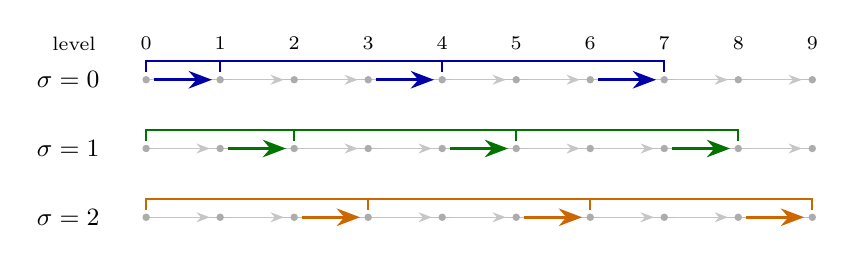
\begin{tikzpicture}[x=.94cm,y=.74cm,>=Stealth,font=\small]
 \foreach \i in {0,...,9}
   \node[font=\scriptsize] at (\i,.62) {\(\i\)};
 \node[anchor=east,font=\scriptsize] at (-.55,.62) {level};
 \foreach \sig/\col in {0/blue!65!black,1/green!45!black,2/orange!80!black}{
   \pgfmathsetmacro{\yy}{-1.18*\sig}
   \node[anchor=east] at (-.5,\yy) {\(\sigma=\sig\)};
   \draw[gray!50] (0,\yy)--(9,\yy);
   \foreach \i in {0,...,8}{
     \pgfmathtruncatemacro{\rr}{mod(\i,3)}
     \ifnum\rr=\sig\relax
       \draw[->,very thick,\col] (\i+.1,\yy)--(\i+.89,\yy);
     \else
       \draw[->,gray!45] (\i+.14,\yy)--(\i+.86,\yy);
     \fi
   }
   \foreach \i in {0,...,9}
     \fill[gray!65] (\i,\yy) circle (1.35pt);
   \pgfmathtruncatemacro{\first}{1+\sig}
   \draw[\col,thick] (0,\yy+.13)--(0,\yy+.32)
     --(\first,\yy+.32)--(\first,\yy+.13);
   \foreach \b in {0,1}{
     \pgfmathtruncatemacro{\aa}{\first+3*\b}
     \pgfmathtruncatemacro{\bb}{\aa+3}
     \draw[\col,thick] (\aa,\yy+.13)--(\aa,\yy+.32)
       --(\bb,\yy+.32)--(\bb,\yy+.13);
   }
 }
\end{tikzpicture}

\medskip
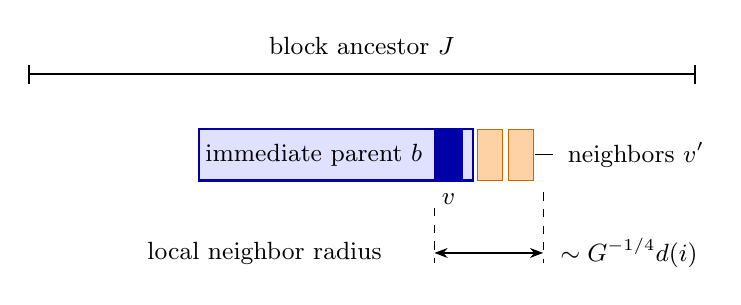
\begin{tikzpicture}[x=.94cm,y=1cm,font=\small,>=Stealth]
 \draw[thick] (0,0)--(9,0);
 \draw[thick] (0,-.12)--(0,.12) (9,-.12)--(9,.12);
 \node[above] at (4.5,.13) {block ancestor \(J\)};
 \fill[blue!12] (2.3,-1.35) rectangle (6,-.7);
 \draw[blue!65!black,thick] (2.3,-1.35) rectangle (6,-.7);
 \node at (3.85,-1.025) {immediate parent \(b\)};
 \fill[blue!65!black] (5.48,-1.35) rectangle (5.86,-.7);
 \node[below] at (5.67,-1.4) {\(v\)};
 \foreach \aa in {6.06,6.48}{
   \fill[orange!35] (\aa,-1.35) rectangle (\aa+.34,-.7);
   \draw[orange!80!black] (\aa,-1.35) rectangle (\aa+.34,-.7);
 }
 \node[anchor=west] at (7.15,-1.02) {neighbors \(v'\)};
 \draw[thin] (6.84,-1.02)--(7.08,-1.02);
 \draw[dashed] (5.48,-1.7)--(5.48,-2.4);
 \draw[dashed] (6.95,-1.5)--(6.95,-2.4);
 \draw[<->] (5.48,-2.27)--(6.95,-2.27);
 \node[anchor=west] at (7.05,-2.27) {\(\sim G^{-1/4}d(i)\)};
 \node[anchor=east] at (4.9,-2.27) {local neighbor radius};
\end{tikzpicture}
\caption{Shifted blocks and boundary masses, schematically.
The upper diagram uses \(K=3\). Each shift starts with \(1+\sigma\)
transitions and then uses blocks of \(K\) transitions; colored arrows
are the final transitions for that shift.
At a final transition \(i\to i+1\), the mass \(m_v\) includes all of
\(n_b\) and the masses of neighboring children outside \(b\) but inside
\(J\). The neighbor radius is determined by the immediate scale \(d(i)\),
even when \(J\) begins much earlier. Neither diagram is to scale.}
\label{fig:shifted-blocks}
\end{figure}


For $\zeta=(\zeta_0,\ldots,\zeta_{K-1})\in\C^K$ and nonempty $v$ at
level $i+1$, put
\begin{equation}
 w_v(\zeta,z)
 =\exp\!\left(\zeta_{i\bmod K}\log\frac{n_v(z)}{m_v(z)}\right).
 \label{hier:analytic-transition}
\end{equation}
All logarithms in this formula are real logarithms of positive numbers.
Thus the weights are entire functions of $\zeta$ and have modulus at
most one when all $\Re\zeta_\sigma\ge0$.

\subsection{The analytic family and its block comparisons}

For a nonempty node $v$ at level $h$, define the $\mathcal H$-valued
analytic amplitude by
\begin{equation}
 A_v(\zeta,z)
 =\sum_{\substack{s:s_{T(s)}\in v\\ k_s\ge h}}
 q_{T(s)}(z)\phi_s(z)\,
 n_{v_{k_s}(T(s))}(z)^{-\mu/K}
 \prod_{i=h}^{k_s-1}w_{v_{i+1}(T(s))}(\zeta,z).
 \label{eq:src-15}
\end{equation}
The condition $k_s\ge h$ already ensures eligibility of $T(s)$ at $v$.
The empty product is one.  This single definition is used for every
shift.  At fixed $z$, it is a finite sum of entire $\mathcal H$-valued
functions of $\zeta$.

We first exhibit two algebraic uses of this common family.  For the block
comparison, temporarily fix a shift $\sigma$ and parameters satisfying
\begin{equation}
 \Re\zeta_\sigma=\mu,
 \qquad \Re\zeta_{\sigma'}=0\quad(\sigma'\ne\sigma),
 \qquad \norm{\Im\zeta}_2\le L^2.
 \label{hier:vertex-parameters}
\end{equation}
We refer to this choice of real parts as the vertex corresponding to
$\sigma$.  Write
$i_j=i_j^\sigma$ and $\rho_j=d(i_j)$.  Thus
\begin{equation}
 G\le\frac{\rho_j}{\rho_{j+1}}\le B,
 \label{hier:block-ratio}
\end{equation}
including the first, possibly shorter, block.

For a nonempty $J\in\mathcal G_{i_j}^\vartheta$, call its nonempty
descendants at level $i_{j+1}$ its \emph{block children}.  For such a block child $c$,
all packets entering $A_c$ have the same transition factor from $J$ to
$c$.  Denote it by
$\lambda_c=\prod_{i=i_j}^{i_{j+1}-1}w_{v_{i+1}}$, along that descendant
path.  Only the last transition of this block has a nonzero real
exponent.  Separating packets according to whether their stopping level
precedes $i_{j+1}$ therefore gives the exact identity
\begin{equation}
 A_J=\sum_{\substack{c\subset J\\c\in\mathcal G_{i_{j+1}}^\vartheta}}
                 \lambda_c A_c+B_J,
 \qquad
 |\lambda_c|=\left(\frac{n_c}{m_c}\right)^\mu.
 \label{eq:src-18}
\end{equation}
The remainder $B_J$ is precisely the sum in \eqref{eq:src-15} over
$i_j\le k_s<i_{j+1}$.  Its assigned tops need not lose eligibility at
the end of the block.  Thus residual packets and lost top mass are
different parts of the block decomposition.

For each nonempty $J$, we add the mass to the normalized $p$-th power
of the amplitude.  The resulting positive amount $V_J$ and its
multiplicative comparison factor $\beta_J$ are
\begin{equation}
 V_J=n_J+n_J^{\alpha-p}\norm{A_J}_{\mathcal H}^p,
 \qquad
 \beta_J=
 \frac{V_J}{n_J+\sum_c n_c^{\alpha-p}\norm{A_c}_{\mathcal H}^p}.
 \label{eq:src-19}
\end{equation}
We use $\beta_J^0$ for the same ratio with $B_J$ omitted only in the
numerator.  The mass baseline makes $V_J$ and every denominator positive,
including when all its block-child amplitudes vanish.  The sum is over
the nonempty descendants at the end of the block.  Equivalently, the
denominator is the lost eligibility mass $n_J-\sum_c n_c$ plus the
block-child amounts $\sum_c V_c$.  This is the comparison later used
in the exact path expansion.

At any one spatial point, abbreviate $n=n_J$ and normalize the child
amplitudes by
\begin{equation}
 l_c=\frac{n_c}{n},\qquad
 X_c=n_c^{\mu-1}A_c,\qquad
 \beta_J^0=
  \frac{1+\norm{\sum_c l_c^{1-\mu}\lambda_c X_c}_{\mathcal H}^p}
       {1+\sum_c l_c\norm{X_c}_{\mathcal H}^p}.
 \label{eq:src-25}
\end{equation}
The ratio follows by dividing \eqref{eq:src-19} by $n$ and using
$p\mu=\alpha-1$.  Also $\sum_c l_c\le1$.  This is a pointwise identity:
the masses, scalar factors, and vectors still vary with the spatial
point.  The vector sum in its numerator is the weighted child sum whose
phase motion we will compare with the weighted child energies in the
denominator.

The boundary mass $m_c$ is designed to pay for selecting separated
children in that comparison.  At the final transition of this block put
$i=i_{j+1}-1$ and
\begin{equation}
 Q=G^{-1/4}d(i)=G^{3/4}\rho_{j+1}.
 \label{hier:child-separation}
\end{equation}
Fix one spatial point and choose any finite subfamily $\mathcal C$ of
nonempty block children.  Join distinct $c,c'\in\mathcal C$ when
$\dist(c,c')<Q$.  Give the children independent exponential clocks of
rates $n_c$, and retain a child when its clock rings before those of all
its neighbors.  The rates are positive.  The clocks have no ties with
probability one, and the retained intervals have pairwise distance at
least $Q$.  The retention probability of $c$ is
\begin{equation}
 \pi_c=\int_0^\infty n_c e^{-n_ct}
              \prod_{c'\sim c}e^{-n_{c'}t}\,\dd t
       =\frac{n_c}{n_c+\sum_{c'\sim c}n_{c'}}
       \ge\frac{n_c}{m_c}.
 \label{pred:retention-probability}
\end{equation}
To see the inequality, let $b$ be the immediate parent of $c$.  The
eligible top sets of $c$ and its competitors inside $b$ are disjoint
subsets of $\mathcal T(b)$, so their masses sum to at most $n_b$.
Every competitor outside $b$ lies inside $J$ and within
$Q=G^{-1/4}d(i)$ of $c$, so its mass is included among the additional
terms of $m_c$ in \eqref{eq:src-14}.  Thus $m_c$ bounds the entire
competing mass even when only a subfamily of children is used.

Multiplying the coefficient of a retained child by $\pi_c^{-1}$ reconstructs its original
coefficient in expectation.  The corresponding expected $r_*$-power
cost is
\[
 \E\!\left[\one_{\{c\text{ retained}\}}\pi_c^{-1}\right]=1,
 \qquad
 \E\!\left[\one_{\{c\text{ retained}\}}\pi_c^{-r_*}\right]
       =\pi_c^{1-r_*}.
\]
The coefficient exponent in \eqref{eq:src-18} matches this cost
exactly.  The identities $r_*(1-\mu)=1$ and $\mu r_*=r_*-1$ give
\begin{equation}
 \pi_c^{1-r_*}|\lambda_c|^{r_*}
   =\left(\frac{n_c/m_c}{\pi_c}\right)^{r_*-1}\le1.
 \label{hier:selection-cancellation}
\end{equation}
The first identity also turns $l_c^{r_*(1-\mu)}$ into $l_c$, the weight
in the denominator of \eqref{eq:src-25}.  The later snapshot construction
will use this selection for the child vectors it retains and check the
remaining hypotheses of the finite Fourier estimate.

The same analytic family has a second algebraic use at the equal-coordinate
parameter
\[
 \zeta^{\mathrm c}=(\mu/K,\ldots,\mu/K).
\]
Let $v$ be a root and let $s$ be a packet contributing to $A_v$, with
$T=T(s)$.  Apart from the factor $q_T\phi_s$, the coefficient of $s$ in
$n_v^{\mu/K}A_v(\zeta^{\mathrm c},z)$ is
\[
 n_v^{\mu/K}n_{v_{k_s}(T)}^{-\mu/K}
       \prod_{i=0}^{k_s-1}
        \left(\frac{n_{v_{i+1}(T)}}{m_{v_{i+1}(T)}}\right)^{\mu/K}.
\]
Cancelling consecutive eligible masses identifies it as
\begin{equation}\label{eq:src-30}
 \kappa_s
   =\prod_{i=0}^{k_s-1}
       \left(\frac{n_{v_i(T)}}{m_{v_{i+1}(T)}}\right)^{\mu/K},
 \qquad T=T(s).
\end{equation}
The empty product is one, and each factor lies in $(0,1]$ by
\eqref{eq:src-14}.  Thus for each root the equal-coordinate value produces
its portion of the masked packet sum with only these boundary ratios in
its coefficients.  The
remaining tasks are to estimate the vertex values, interpolate those
estimates to $\zeta^{\mathrm c}$, and remove the boundary ratios by
averaging the angular-grid translation.

\subsection{Full-root variation and amplitude bounds}

We now leave the temporary vertex specialization and return to the general
range $0\le\Re\zeta_\sigma\le\mu$ for every coordinate, with arbitrary
imaginary parts.  The following bounds control the endpoint weights
without a loss proportional to the number of levels.  Along one eligible
top path, write $n_i=n_{v_i(T)}$ and
\begin{equation}
 P_i=\log\frac{n_i}{n_{i+1}},
 \qquad
 R_i=\log\frac{m_{v_{i+1}(T)}}{n_{i+1}}.
 \label{hier:positive-logs}
\end{equation}
Both are nonnegative as long as the top remains eligible at level $i+1$.

\begin{lemma}[Full-root variation bound]
\label{hier:weight-variation}
Fix an eligible path from a root $v_0(T)$ through level $k$.  At every
spatial point,
\begin{equation}
 \sum_{i=0}^{k-1}R_i
 \le K\log\frac{n_{v_0(T)}}{n_{v_k(T)}},
 \qquad
 \sum_{i=0}^{k-1}P_i
 =\log\frac{n_{v_0(T)}}{n_{v_k(T)}}.
 \label{hier:full-root-telescope}
\end{equation}
For a fixed starting level $h\le k_T$, define, for $h\le k\le k_T$,
\[
 \omega_{T,h,k}(\zeta,z)
 =n_{v_k(T)}(z)^{-\mu/K}
   \prod_{i=h}^{k-1}w_{v_{i+1}(T)}(\zeta,z).
\]
If $0\le\Re\zeta_\sigma\le\mu$ for every $\sigma$, then the supremum
plus total variation of this sequence, with the endpoint $k$ varying,
is bounded by
\begin{equation}
 \sup_{h\le k\le k_T}|\omega_{T,h,k}|
 +\sum_{k=h}^{k_T-1}
       |\omega_{T,h,k+1}-\omega_{T,h,k}|
 \le C h_T^{-\mu/K}
 \left[1+K(1+\norm{\zeta}_2)
                   \log\frac{n_{v_0(T)}}{h_T}\right].
 \label{eq:src-16}
\end{equation}
The same bound holds upon restricting the endpoints to a subinterval.
\end{lemma}

\begin{proof}
Fix a shift $\sigma$.  For the transitions $i\equiv\sigma\pmod K$
with $i<k$, \eqref{hier:boundary-mass-bounds} gives
\[
 R_i\le\log\frac{n_{a(i)}}{n_{i+1}}.
\]
For this fixed shift, the intervals of levels $[a(i),i+1]$ are successive
blocks starting at zero.  Their logarithms telescope.  The endpoint of
the last completed block is at most $k$, so the sum is at most
$\log(n_0/n_k)$, by monotonicity of the masses.  Summing over the $K$
shifts proves the first inequality in
\eqref{hier:full-root-telescope}.  The second is an ordinary telescope.
This is a full-root bound.  In particular, it remains applicable to
weights occurring on a later segment even when another shift's block
starts before that segment.

Set $a=\mu/K$, solely for this proof, and use the specified logarithm
\[
 L_k=-a\log n_k-\sum_{i=h}^{k-1}\zeta_{i\bmod K}R_i,
 \qquad \omega_{T,h,k}=e^{L_k}.
\]
Its increment is
\begin{equation}
 L_{k+1}-L_k=aP_k-\zeta_{k\bmod K}R_k.
 \label{hier:log-weight-increment}
\end{equation}
Since $n_k\ge h_T$ and all real transition exponents are nonnegative,
$|e^{L_k}|\le h_T^{-a}$.  For any complex $A,B$,
\[
 |e^B-e^A|
 \le |B-A|\int_0^1|e^{(1-t)A+tB}|\,\dd t
 \le |B-A|\max(|e^A|,|e^B|).
\]
Using this inequality for adjacent logarithms and then
\eqref{hier:full-root-telescope} proves \eqref{eq:src-16}.  Notice that
the exponential of the sum of the absolute logarithmic increments has
not been used.  Such an exponential would be unsuitable when $h_T$ is
very small.
\end{proof}

\begin{lemma}[Amplitude bounds]
\label{hier:amplitudes}
On $Z_0$, for $0\le\Re\zeta_\sigma\le\mu$,
\begin{equation}
 \norm{A_v(\zeta,z)}_{\mathcal H}
 \le L^C(1+\norm{\zeta}_2)n_v(z).
 \label{eq:src-17}
\end{equation}
More precisely, the contribution of any one eligible top $T$ to $A_v$,
also when restricted to any interval of packet lengths, is bounded by
\begin{equation}
 L^C(1+\norm{\zeta}_2)|q_T(z)|h_T(z)^4.
 \label{hier:individual-amplitude}
\end{equation}
If all eligible tops of $v$ are insignificant at $z\in Z_0$, then
\begin{equation}
 \norm{A_v(\zeta,z)}_{\mathcal H}
 \le L^C(1+\norm{\zeta}_2)e^{-L\log L}n_v(z).
 \label{hier:insignificant-amplitude}
\end{equation}
\end{lemma}

\begin{proof}
For vectors $f_h,\ldots,f_k$ and scalars $\omega_h,\ldots,\omega_k$,
summation by parts gives
\begin{equation}
 \norm{\sum_{i=h}^k\omega_i f_i}
 \le
 \left(|\omega_k|+\sum_{i=h}^{k-1}|\omega_{i+1}-\omega_i|\right)
 \max_{h\le j\le k}\norm{\sum_{i=h}^j f_i}.
 \label{hier:summation-by-parts}
\end{equation}
Group the packets assigned to $T$ according to their stopping level.
The resulting initial sums, or the sums obtained after restricting to an
interval of packet lengths, are interval partial sums of the original
top's length sequence.  By \eqref{eq:src-11} and the fact that the
$K_0$-dilated weight is at least the corresponding $K_1$-dilated weight,
their norm at $z\in Z_0$ is at most $L^C h_T(z)^8$.  The mask $q_T(z)$
is common to this whole top.  Apply
\eqref{hier:summation-by-parts} and \eqref{eq:src-16}.

To see that the logarithmic factor can be absorbed uniformly, use
\eqref{eq:src-12} and $\log N\le2L$.  Since $n_{v_0(T)}\le n$ and
$h_T\le C_3$,
\[
 0\le\log\frac{n_{v_0(T)}}{h_T}
 \le C L+\log^+\frac1{h_T}.
\]
Here and below $\log^+x=\max(0,\log x)$.  Also $\mu/K<1$.  The
elementary boundedness of $x^\delta\log^q(1/x)$ on $(0,1]$, for fixed
$\delta>0$ and fixed $q$, shows that
\[
 h_T^{8-\mu/K}
 \left[1+K(1+\norm{\zeta}_2)
                    \log\frac{n_{v_0(T)}}{h_T}\right]
 \le L^C(1+\norm{\zeta}_2)h_T^4.
\]
This proves \eqref{hier:individual-amplitude}.  Summing over the eligible
tops and using $h_T^4\le C_3^3h_T$ proves \eqref{eq:src-17}.
For insignificant tops, the mask estimate after \eqref{eq:src-8} gives
$|q_T|\le e^{-L\log L}$.  Applying the same summation proves
\eqref{hier:insignificant-amplitude}.
\end{proof}

\subsection{Spatial meshes for prediction}

Return to a fixed shift $\sigma$ and a vertex parameter satisfying
\eqref{hier:vertex-parameters}.  Write $i_j=i_j^\sigma$ and
$\rho_j=d(i_j)$ as in the block comparison above, and take
$J\in\mathcal G_{i_j}^\vartheta$.  Its block children and their factors
are those in \eqref{eq:src-18}.
Let $R$ be any top eligible in $J$, and parametrize a line of slope
$s_R$ by $z(x)=(x,y_*+s_Rx)$.  On this line use one nested dyadic grid in
the parameter $x$, at lengths
\begin{equation}
 H_j=\frac{w}{\rho_{j+1}\sqrt G},
 \qquad H_{-1}=\frac{w}{\rho_0\sqrt G}.
 \label{eq:src-20}
\end{equation}
These are dyadic lengths because $w,d(0),G$, and $\sqrt G$ are dyadic.
They increase with $j$.  The grids can, for example, have common origin
zero.  Each $H_j$ cell is a union of $H_{j-1}$ cells.

\subsection{Positive-mass motion and the locality of other shifts}

\begin{lemma}[Mass motion]
\label{hier:mass-motion}
Fix $R,J,j$ as above and an interval $I$ of horizontal length $H_j$ on a
line of slope $s_R$.  Consider the masses $n_J,n_c,m_c$ in
\eqref{eq:src-18}, the masses used in the factors $\lambda_c$, and those
used in any endpoint multiplier of a packet contributing to $A_c$.
Each such mass, and each of its positive subset-complement differences
used below, is a sum of weights of tops $T$ satisfying
\begin{equation}
 |s_T-s_R|\le C\rho_j,
 \qquad d_T\le\rho_j/B^2.
 \label{hier:motion-locality}
\end{equation}
There is an absolute constant $C$ such that, with
$\varepsilon_{\mathrm{mov}}=C G^{-1/2}$, every nonzero such mass $a$ satisfies
\begin{equation}
 |\partial_x\log a|\le\frac{\varepsilon_{\mathrm{mov}}}{H_j}
 \quad\text{almost everywhere on }I.
 \label{hier:mass-log-derivative}
\end{equation}
If $r=a/(a+b)$ is one of the ratios of a submass to its containing mass,
then
\begin{equation}
 |\partial_x\log r|
 \le\frac{2\varepsilon_{\mathrm{mov}}}{H_j}(1-r)
 \le\frac{2\varepsilon_{\mathrm{mov}}}{H_j}(-\log r).
 \label{hier:ratio-derivative}
\end{equation}
When $b=0$, the ratio is identically one and its derivative is zero.
In particular, nonzero $n_J-n_c$ and $m_c-n_c$ have the relative motion
bound \eqref{hier:mass-log-derivative}.  All these masses vary by a
factor $1+O(G^{-1/2})$ across $I$.

For the parameters \eqref{hier:vertex-parameters}, the block
factors also satisfy, for $x,x_0\in I$,
\begin{equation}
 \left|\frac{\lambda_c(x)}{\lambda_c(x_0)}-1\right|
 \le G^{-c_0}
 \label{hier:complex-transition-motion}
\end{equation}
for some absolute $c_0>0$ and all sufficiently large $L$.
\end{lemma}

\begin{proof}
All descendants of $J$ have slopes inside $J$, so their top slopes are
within $\rho_j$ of $s_R$.  Their eligibility cutoffs are at most
$\rho_j/B^2$.  A mass in an additional boundary term
\eqref{eq:src-14} at a transition $i\ge i_j$ can come from an interval
outside $J$, because the block associated to another shift can start
before $i_j$.  However, that interval is within
$G^{-1/4}d(i)$ of the relevant child and has width $d(i+1)$.
The relevant child is a descendant of $J$, and $d(i)\le\rho_j$.
Hence every added slope is within $C\rho_j$ of $s_R$.  The tops in an
added interval have precision at most $d(i+1)/B^2$; those in the
immediate-parent mass have precision at most $d(i)/B^2$.
This proves \eqref{hier:motion-locality}, including for weights below
the block.  Taking a difference of the relevant nested top sets preserves
the same property.  This argument uses the neighbor radius at the
immediate transition, rather than the possibly larger width of the other
shift's block ancestor.

In normalized coordinates of a top $T$, horizontal motion along $s_R$
has velocities $1/l_T$ and $(s_R-s_T)/W$.  Differentiating
\eqref{eq:src-5}, using the Lipschitz property of the absolute value at
almost every point, gives
\[
 |\partial_x\log h_T|
 \le C\left(\frac1{l_T}+\frac{|s_R-s_T|}{W}\right)
 \le C\left(\frac{\rho_j}{B^2w}+\frac{\rho_j}{mw}\right).
\]
The factor $K_0^{-1}$ available from the dilation is not needed.
Multiplying by $H_j$ and using \eqref{hier:block-ratio} yields
\[
 H_j|\partial_x\log h_T|
 \le\frac C{\sqrt G}
       \left(\frac{B}{B^2}+\frac Bm\right)
 \le C G^{-1/2}.
\]
For a positive sum $a=\sum_T h_T$, its logarithmic derivative is the
weighted average of the logarithmic derivatives of the summands.
This proves \eqref{hier:mass-log-derivative}, also for positive
differences, which are such sums by their set interpretation.

If $a,b>0$, direct differentiation gives
\[
 \partial_x\log\frac a{a+b}
 =\frac b{a+b}\bigl(\partial_x\log a-\partial_x\log b\bigr).
\]
This proves \eqref{hier:ratio-derivative}; the inequality
$1-r\le-\log r$ holds for $0<r\le1$.  If the complementary top set is
empty, $r=1$ everywhere.  In particular, writing $q_r=-\log r\ge0$,
\begin{equation}
 |\partial_x q_r|\le\frac{2\varepsilon_{\mathrm{mov}}}{H_j}q_r,
 \qquad
 e^{-2\varepsilon_{\mathrm{mov}}}q_r(x_0)
 \le q_r(x)\le e^{2\varepsilon_{\mathrm{mov}}}q_r(x_0)
 \quad(x,x_0\in I).
 \label{hier:loss-motion}
\end{equation}
The inequalities remain valid for an identically zero loss.

Finally, a block factor is a product of at most $K$ transition factors.
The simpler bound $|\partial_x\log r|\le2\varepsilon_{\mathrm{mov}}/H_j$ shows that
its specified complex logarithm changes by at most
$C K(1+\norm{\zeta}_2)G^{-1/2}$.  For
\eqref{hier:vertex-parameters} this is $L^C G^{-1/2}$ and tends to zero
faster than any negative fixed power of $L$.  Exponentiating proves
\eqref{hier:complex-transition-motion} after decreasing $c_0$.
This last argument does not require any bound on the size of a
logarithmic loss itself.
\end{proof}

\subsection{Variation of moving endpoint weights}

The next estimate makes explicit why the motion of the analytic weights
can be controlled from a single point, even for very small $h_T$.
For a finite scalar sequence $a=(a_k)$ let
\[
 \norm{a}_{\mathrm{BV}}
 =\sup_k|a_k|+\sum_k|a_{k+1}-a_k|.
\]
Only this elementary finite-sequence norm is used here.

\begin{lemma}[Moving weights]
\label{hier:moving-weights}
In the setting of \Cref{hier:mass-motion}, fix a top $T$ contributing to
$A_c$, and take endpoint weights $\omega_k=\omega_{T,i_{j+1},k}$.
If $z_0\in I\cap Z_0$ and the parameters satisfy
\eqref{hier:vertex-parameters}, then, uniformly for $z'\in I$,
\begin{align}
 \norm{(\omega_k(z'))_k}_{\mathrm{BV}}
 &\le L^C h_T(z_0)^{-4},
 \label{hier:moving-weight-bv}\\
 \norm{(\omega_k(z')-\omega_k(z_0))_k}_{\mathrm{BV}}
 &\le G^{-1/2}L^C h_T(z_0)^{-4}.
 \label{hier:moving-weight-difference}
\end{align}
Both conclusions hold for any interval of endpoints.  Neither assumes
that $z'$ belongs to $Z_0$.
\end{lemma}

\begin{proof}
Parametrize the interval by its horizontal coordinate $x$, and write
$h=i_{j+1}$ and $a=\mu/K$ in this proof.  Use $P_i,R_i$ from
\eqref{hier:positive-logs} for $h\le i<k_T$.  By
\eqref{hier:loss-motion}, each of these nonnegative losses is comparable
throughout $I$ to its value at $x_0$, with factor
$e^{O(\varepsilon_{\mathrm{mov}})}$, and its absolute derivative is bounded by
$C\varepsilon_{\mathrm{mov}}/H_j$ times itself.  Define
\[
 \mathcal B(x)=\sum_{i=h}^{k_T-1}
                    \bigl(aP_i(x)+|\zeta_{i\bmod K}|R_i(x)\bigr).
\]
It follows that $\mathcal B(x)\le e^{C\varepsilon_{\mathrm{mov}}}\mathcal B(x_0)$.
By the full-root bound,
\begin{equation}
 \mathcal B(x_0)
 \le C K(1+\norm{\zeta}_2)
                 \log\frac{n_{v_0(T)}(z_0)}{h_T(z_0)}.
 \label{hier:moving-loss-budget}
\end{equation}
The full-root mass is used only at the snapshot in this inequality; its
spatial derivative is not needed.

Let $L_k=\log\omega_k$ be the specified logarithm in the proof of
\Cref{hier:weight-variation}, and put $q_k=\partial_x L_k$.
Equation~\eqref{hier:log-weight-increment} and the mass derivative
bound imply
\begin{align*}
 \sup_k|q_k|
 &\le\frac{C\varepsilon_{\mathrm{mov}}}{H_j}
                  \bigl(a+\mathcal B(x)\bigr),\\
 \sum_k|q_{k+1}-q_k|
 &\le\frac{C\varepsilon_{\mathrm{mov}}}{H_j}\mathcal B(x).
\end{align*}
For example, the initial term is
$q_h=-a\partial_x\log n_h$, and subsequent differences are the
derivatives of $aP_i-\zeta_{i\bmod K}R_i$.  At every point of $I$,
\[
 \sup_k|\omega_k(x)|\le h_T(x)^{-a}
 \le e^{a\varepsilon_{\mathrm{mov}}}h_T(z_0)^{-a}.
\]
The complex-exponential estimate used for
\eqref{eq:src-16} therefore gives
\[
 \norm{\omega(x)}_{\mathrm{BV}}
 \le C h_T(z_0)^{-a}\bigl(1+\mathcal B(x_0)\bigr).
\]

For finite sequences the product rule for differences gives
\[
 \norm{ab}_{\mathrm{BV}}
 \le \sup_k|a_k|\norm{b}_{\mathrm{BV}}
       +\sup_k|b_k|\sum_k|a_{k+1}-a_k|.
\]
Using $\partial_x\omega_k=\omega_k q_k$ and the preceding estimates
yields
\begin{equation}
 \norm{\partial_x\omega(x)}_{\mathrm{BV}}
 \le\frac{C\varepsilon_{\mathrm{mov}}}{H_j}
 h_T(z_0)^{-a}\bigl(1+\mathcal B(x_0)\bigr)^2.
 \label{hier:weight-derivative-bv}
\end{equation}
The functions involved are absolutely continuous on the line.  Integrate
\eqref{hier:weight-derivative-bv} between $x_0$ and $x'$, over distance
at most $H_j$, and use the triangle inequality for the finite-sequence
norm.  This proves the difference bound with right side
$C\varepsilon_{\mathrm{mov}} h_T(z_0)^{-a}(1+\mathcal B(x_0))^2$.

At the snapshot, \eqref{eq:src-12},
\eqref{hier:vertex-parameters}, and
\eqref{hier:moving-loss-budget} bound the last expression by
$G^{-1/2}L^C h_T(z_0)^{-4}$.  Indeed the only possible nonpolynomial
quantity is $\log^+(1/h_T(z_0))$, whose square is absorbed by the
difference between exponents $a<1$ and $4$.  The same argument proves
\eqref{hier:moving-weight-bv}.  There is no assumption that
$G^{-1/2}\mathcal B(x_0)$ is small: very small $h_T$ is allowed, and
only a polynomial in its logarithm has appeared.
\end{proof}

\subsection{Amplitude motion from one good snapshot}

\begin{lemma}[Predictable amplitude motion]
\label{hier:amplitude-motion}
Fix a block child $c$ of $J$, a path top $R$ eligible in $J$,
and an $H_j$ cell on a line of slope $s_R$.  Let $t_c$ be the angular
center of $c$.  If $z_0\in Z_0$ lies in that cell and
$z'=z_0+(b,s_Rb)$ is any other point in the cell, then, for the parameters \eqref{hier:vertex-parameters},
\begin{equation}
 \norm{A_c(\zeta,z')-\mathcal D_c(b)A_c(\zeta,z_0)}_{\mathcal H}
 \le G^{-c_0}n_c(z_0),
 \qquad
 \mathcal D_c(b)_{\nu\nu}
 =\exp\bigl(i(s_R-t_c)\eta_\nu b\bigr).
 \label{eq:src-21}
\end{equation}
Here $c_0>0$ is absolute and may also be used, after decreasing it, in
\eqref{hier:complex-transition-motion}.  The estimates hold at all
displaced points in the cell, not just its points in $Z_0$.
\end{lemma}

\begin{proof}
Fix one top $T$ contributing to $A_c$.  Its contributing packets have
$k_s\ge i_{j+1}$, hence
\begin{equation}
 \ell_s\ge l_*:=\frac{B^2w}{\rho_{j+1}},
 \qquad l_T\ge l_*.
 \label{hier:predictable-length}
\end{equation}
Also $s_T\in c$, so $|s_T-t_c|\le\rho_{j+1}/2$, while
$|s_T-s_R|\le C\rho_j$.

Consider any interval partial sum $S$ of these unweighted packets on
$T$.  The good-snapshot estimates \eqref{eq:src-11}, including their
demodulated vertical-derivative and vertical-neighborhood versions, bound
$S$ and $W(\partial_y-i\eta_\nu)S_\nu$ by
$L^Ch_T(z_0)^8$ throughout the vertical neighborhood of radius $W$
at $z_0$.  Put $v=(s_R-s_T)b$ and first move to
$z_1=z_0+(0,v)$.  Since
\[
 |v|\le C\rho_jH_j\le\frac{CBw}{\sqrt G}\ll W,
\]
the fundamental theorem of calculus after componentwise demodulation
gives
\[
 \norm{S(z_1)-\operatorname{diag}(e^{i\eta_\nu v})S(z_0)}
 \le L^Ch_T(z_0)^8\frac{|v|}{W}
 \le G^{-1/2}L^Ch_T(z_0)^8.
\]
Next move from $z_1$ to $z'$ along slope $s_T$ by horizontal distance
$b$.  The nonexceptional horizontal derivative estimate in
\Cref{conc:top-good}, applied to lengths at least $l_*$, bounds this
change by
\[
 L^Ch_T(z_0)^8\frac{|b|}{l_*}
 \le G^{-1/2}L^Ch_T(z_0)^8.
\]
To justify its spatial weight here, the two displacements change the
normalized coordinates of $T$ by at most
$C/(B^2\sqrt G)+CB/(m\sqrt G)$.  Its weight at every intermediate
point is therefore comparable to $h_T(z_0)$.  If the derivative estimate
is expressed using the smaller dilation $K_1$, that weight is bounded
above by the $K_0$-dilated weight used here.  No good-point estimate at
$z_1$ or $z'$ has been invoked for this horizontal move.

The replacement of $s_T$ by $t_c$ in the diagonal phase costs at most
\[
 C|s_T-t_c|\frac{|b|}{w}\norm{S(z_0)}
 \le G^{-1/2}L^Ch_T(z_0)^8,
\]
because $\eta_\nu\asymp w^{-1}$ uniformly in $\nu$.
This proves, uniformly over the interval partial sum,
\begin{equation}
 \norm{S(z')-\mathcal D_c(b)S(z_0)}
 \le G^{-1/2}L^Ch_T(z_0)^8.
 \label{hier:unweighted-motion}
\end{equation}

The same bound holds with the mask $q_T$ multiplying $S$ at its own
evaluation point.  Indeed $|q_T|\le1$, and its formula
\eqref{eq:src-8}, together with boundedness of the derivative of sinc,
gives
\[
 |q_T(z')-q_T(z_0)|
 \le L^C\left(\frac{|b|}{l_T}
                    +\frac{|s_R-s_T|\,|b|}{W}\right)
 \le G^{-1/2}L^C.
\]
Combining this with the snapshot bound for $S$ proves the masked version
of \eqref{hier:unweighted-motion}.  This estimate uses absolute motion
of the mask and does not divide by $q_T$, which may vanish.

Group the masked packets by stopping level and denote their sums by
$f_k(z)$.  Their weighted contribution to the difference in
\eqref{eq:src-21} is
\begin{align*}
 &\sum_k\omega_k(z')
       \bigl(f_k(z')-\mathcal D_c(b)f_k(z_0)\bigr)\\
 &\hspace{15mm}
 +\sum_k\bigl(\omega_k(z')-\omega_k(z_0)\bigr)
                        \mathcal D_c(b)f_k(z_0).
\end{align*}
All interval partial sums of the first parenthesis have norm at most
$G^{-1/2}L^Ch_T(z_0)^8$, by the masked version of
\eqref{hier:unweighted-motion}.  The snapshot partial sums in the second
line have norm at most $L^Ch_T(z_0)^8$.  Apply
\eqref{hier:summation-by-parts} to both lines, then
\eqref{hier:moving-weight-bv} and
\eqref{hier:moving-weight-difference}.  The result for this top is at
most $G^{-1/2}L^Ch_T(z_0)^4$.
Sum over the tops eligible in $c$.  Since $h_T^4\le C_3^3h_T$, this is
at most $G^{-1/2}L^Cn_c(z_0)$.  Finally
$\log G\asymp L^{0.7}$ absorbs every fixed power of $L$ into a smaller
positive power of $G$, proving \eqref{eq:src-21}.
\end{proof}

\subsection{One deterministic residual sequence for each path}

We now refine $Z_0$ by a set which depends on the angular translation but
not on $\zeta$.  Its purpose is to make the later residual estimates
available on most of the path weight.  The subsets of packets used in
its definition must be fixed before evaluating a spatial point or
choosing a mass cutoff.

For each possible path top $R$, let
\begin{equation}
 \mathcal P_R
 =\{s:\ell_s\le l_R,\quad
                    |\theta_s-s_R|\le C B^4d_s\},
 \label{hier:reference-packets}
\end{equation}
where the absolute constant is large enough to cover the assigned-top
comparisons below.  Apply the main/error decomposition of
\Cref{conc:line-moments} with reference slope $s_R$ to this fixed
collection.  Denote the resulting positive error sum by
$\mathcal E_R$ and positive main square function by $\mathcal S_R$.
The absolute envelopes can use fixed decay exponents slow enough to
dominate the norms of the unweighted synthesis packets.  There is no
loss in doing so because the packet bounds are available with arbitrarily
large fixed decay exponents.

For each shift $\sigma$, define a second fixed collection
\begin{equation}
 \mathcal Q_{R,\sigma}
 =\bigcup_{\substack{j\ge0\\ i_{j+1}^\sigma\le k_R}}
 \left\{s:
 \begin{array}{l}
 i_j^\sigma\le k_s<i_{j+1}^\sigma,\\
 T(s)\in\mathcal T\bigl(v_{i_{j+1}^\sigma}(R)\bigr)
 \end{array}\right\}.
 \label{hier:deterministic-residual-subset}
\end{equation}
For blocks at whose endpoint $R$ is still eligible, these are the packets
that stop within the block while their assigned tops remain eligible in
the child $v_{i_{j+1}^\sigma}(R)$.  The union takes all such blocks at
once, fixing one packet collection before any spatial point or mass cutoff
is chosen.  Let $\mathcal V_{R,\sigma}$ be the $3$-variation of the
sequence formed by summing $q_{T(s)}\phi_s$ from this collection at each
packet length.  It permits any finite list of disjoint intervals of that
one length sequence.  Subsequent choices of those intervals may depend
on the evaluation point; the collection and its length sequence remain fixed.

Every packet in $\mathcal Q_{R,\sigma}$ satisfies the hypotheses of
\Cref{conc:line-moments} with $t=s_R$ and $l=l_R$.  Indeed,
$k_s<i_{j+1}^\sigma\le k_R$ gives
\begin{equation}
 d_s>\frac{\rho_{j+1}}{B^2}\ge d_R,
 \qquad \ell_s<l_R.
 \label{hier:residual-precision}
\end{equation}
Since $s_{T(s)}$ and $s_R$ are in the same block-child interval of width
$\rho_{j+1}$,
\[
 |\theta_s-s_R|
 \le |\theta_s-s_{T(s)}|+|s_{T(s)}-s_R|
 \le C d_s+\rho_{j+1}\le C B^2d_s\le C B^4d_s.
\]
For later use, if a residual packet only lies in the larger path node
$J=v_{i_j}(R)$ and has $\ell_s\le l_R$, then
$|s_{T(s)}-s_R|\le\rho_j\le B\rho_{j+1}<B^3d_s$; thus it belongs to
$\mathcal P_R$ as well.  These facts explain both choices of fixed
collections.

\begin{lemma}[Good paths]
\label{hier:good-paths}
There is a fixed exponent $C_{\mathrm{path}}$, chosen independently of
the mass cutoff below, such that the following construction is valid.
Call $R$ bad at $z$ if any of
$\mathcal E_R(z),\mathcal S_R(z),\mathcal V_{R,\sigma}(z)$,
$0\le\sigma<K$, exceeds $L^{C_{\mathrm{path}}}$.  Otherwise call it
good at $z$.  For every fixed angular translation,
\begin{equation}
 \sum_R\int_{\R^2}h_R(z)\one_{\{R\text{ bad at }z\}}\,\dd z
 \le S e^{-10L}.
 \label{hier:weighted-bad-paths}
\end{equation}
The constant $10$ may be replaced by any prescribed absolute constant
by increasing the fixed exponent.  The measurable set
\begin{equation}
 Z=Z_\vartheta
 =\left\{z\in Z_0:
       \sum_{R\text{ bad at }z}h_R(z)\le e^{-L}\right\}
 \label{hier:good-set}
\end{equation}
is independent of $\zeta$ and satisfies
\begin{equation}
 |Z_0\setminus Z|\le S e^{-9L}
 \le L^Ce^{-5L}|F|.
 \label{hier:good-set-budget}
\end{equation}
Its removal is therefore allowable in the target estimate
\eqref{eq:src-7}, using the original adjoint sum's $L^2$ bound.
\end{lemma}

\begin{proof}
Fix $R$, a line of slope $s_R$, and any horizontal interval $I$ of length
$l_R$ on that line.  By \Cref{conc:line-moments}, the normalized
$L^b(I)$ norm of each indicated quantity is at most
$C b^C(1+\log B)^C$.  The same bound holds for
$\mathcal V_{R,\sigma}$ because
\eqref{hier:deterministic-residual-subset} is a fixed subset satisfying
\eqref{eq:src-9}.  As $\log B=K\log G$ is bounded by a fixed power of
$L$, this bound is polynomial in $L$ when $b$ is a fixed positive
multiple of $L$.

For clarity, fix an arbitrarily large absolute number $J_0$.  Choose
$b=\lceil L\rceil$ and then a fixed exponent
$C_{\mathrm{path}}$ sufficiently larger than those in the moment bound.
Markov's inequality gives, for all large $L$,
\[
 \begin{aligned}
 &|\{x\in I:\mathcal E_R(x)>L^{C_{\mathrm{path}}}\}|
  +|\{x\in I:\mathcal S_R(x)>L^{C_{\mathrm{path}}}\}|\\
 &\qquad
  +\sum_{\sigma=0}^{K-1}
   |\{x\in I:\mathcal V_{R,\sigma}(x)>L^{C_{\mathrm{path}}}\}|
  \le e^{-J_0L}|I|.
 \end{aligned}
\]
The factor $K+2$ is polynomial and is absorbed by the same choice.
Alternatively one may increase the fixed multiple in the choice of
$b$; neither choice depends on the number of scales or tops.

Partition the whole reference line into intervals of length $l_R$.
Along this line $h_R$ changes by at most an absolute factor on each such
interval, directly from \eqref{eq:src-5}.  Hence the preceding estimate
implies
\[
 \int_I h_R\one_{\{R\text{ bad}\}}\,\dd x
 \le C e^{-J_0L}\int_I h_R\,\dd x.
\]
Sum over the intervals and integrate in the transverse coordinate
$y-s_Rx$; this change of coordinates has determinant one.  Using
\eqref{hier:top-weight-basic} gives
\[
 \int_{\R^2}h_R\one_{\{R\text{ bad}\}}\,\dd z
 \le L^C e^{-J_0L}|R_R|.
\]
Sum over $R$ and take $J_0$ large enough to obtain
\eqref{hier:weighted-bad-paths}.  This establishes the estimate with
its full spatial weight, not only on the central part of $R$.

Markov's inequality applied to the nonnegative sum defining
\eqref{hier:good-set} gives its first measure bound.  Since
$S\le L^C|E|=L^CN^2|F|$ and $N\le e^{2L}$, the second follows.
For example, Cauchy--Schwarz and the previously proved adjoint estimate
give
\[
 \int_{Z_0\setminus Z}\norm{P}
 \le |Z_0\setminus Z|^{1/2}\norm{P}_2
 \le L^Ce^{-5L/2}N|F|,
\]
which is smaller than any required fixed negative power of $L$ times
$N|F|$.  The estimate is applied to the original sum $P$, as required
for exceptional discards.

Finally, all packet collections used here depend only on the finite
geometric data, the angular translation, and the shift.  They do not
depend on $z$, $\zeta$, significance, or a mass cutoff.  Their finite
length variations and the other thresholded quantities are measurable
in $z$.  They are measurable jointly with $\vartheta$ as well: at the
finitely many relevant angular levels, membership of each of the
finitely many top slopes in its interval changes at finitely many
translation endpoints.  On the complementary parameter intervals
all the relevant membership data are fixed.  This also proves the
asserted independence from $\zeta$.
\end{proof}

\subsection{Mass stopping and the exact path expansion}

Choose a cutoff
\begin{equation}
 M=L^{A_M},
 \label{hier:mass-cutoff}
\end{equation}
where the fixed exponent $A_M$ will be taken sufficiently large in the
residual estimates.  Every threshold and exponent in the preceding
lemmas has already been fixed without reference to $A_M$.  Statements
below that use $M$ hold for each such fixed exponent after increasing
the lower threshold for $L$.

For convenience set
\begin{equation}
 C_M=L^{Cp}(1+M)^{\alpha-1},
 \label{hier:stop-cost}
\end{equation}
with a fixed sufficiently large $C$.  Equation~\eqref{eq:src-17} and
$p\mu=\alpha-1$ imply that a node of mass $n_J\le M$ satisfies
\begin{equation}
 V_J\le C_M n_J.
 \label{hier:small-node-amount}
\end{equation}
Indeed $V_J/n_J\le1+L^{Cp}n_J^{\alpha-1}$ for the parameters.

\begin{lemma}[Expansion into top paths]
\label{hier:path-expansion}
Fix $z\in Z$, a root, a shift, and parameters as above.  Starting
from a node with $n_J>M$, expand
\begin{equation}
 V_J=\beta_J
      \left(n_J-\sum_c n_c+\sum_c V_c\right),
 \label{hier:exact-expansion}
\end{equation}
and stop a branch on first reaching a node of mass at most $M$.
At each expanding node, split $n_J-\sum_c n_c$ into the individual
weights of the tops which do not remain eligible at the block endpoint.
At a stopped node split $V_J$ proportionally among its eligible top
weights.  This gives exactly one terminal path for each eligible root
top $R$, with a terminal amount $e_R$ satisfying
\begin{equation}
 0<e_R\le C_Mh_R,
 \qquad
 V_{\mathrm{root}}
 =\sum_R e_R\prod_{J\text{ active on }R\text{'s path}}\beta_J.
 \label{hier:top-path-expansion}
\end{equation}
If $n_{\mathrm{root}}>M$, at least one half of this sum comes from tops
which are good at $z$.  Consequently,
\begin{equation}
 V_{\mathrm{root}}(z)
 \le 2C_M\sum_{\substack{R\text{ eligible at root}\\R\text{ good at }z}}
     h_R(z)\prod_{J\text{ active on }R\text{'s path}}\beta_J(z).
 \label{hier:good-path-domination}
\end{equation}
If $n_{\mathrm{root}}\le M$, \eqref{hier:small-node-amount} applies
instead.
\end{lemma}

\begin{proof}
Identity~\eqref{hier:exact-expansion} follows directly from
\eqref{eq:src-19}, because
$V_c-n_c=n_c^{\alpha-p}\norm{A_c}^p$.  The term
$n_J-\sum_c n_c$ is a sum of top weights by
\eqref{hier:mass-loss}, now between the endpoints of the whole block.
Every top either remains eligible in exactly one block child or loses
eligibility and terminates at $J$.  The construction therefore branches by disjoint
top sets, assigning each top exactly one path.  It terminates after
finitely many blocks even if no mass stop occurs, since no top is
eligible beyond the final level.  At such a final expanding node the
block-child sum is empty and all tops terminate directly.

If $R$ terminates directly at an expanding node, its terminal amount is
$h_R$.  If it reaches a mass-stopped node $c$, the terminal amount is
$(V_c/n_c)h_R$, which is at most $C_Mh_R$ by
\eqref{hier:small-node-amount}.  Repeated use of
\eqref{hier:exact-expansion} proves the equality in
\eqref{hier:top-path-expansion}.

To verify the claim about bad paths, it is useful to normalize the
expansion by actual probabilities.  At an active node define
\[
 D_J=n_J-\sum_c n_c+\sum_cV_c
     =n_J+\sum_c(V_c-n_c)>M.
\]
Choose a block child $c$ with probability $V_c/D_J$, or a directly
terminating top $R$ with probability $h_R/D_J$.  These probabilities sum
to one.  At a mass-stopped node choose an eligible top with probability
$h_R/n_c$.  The probability of a given complete terminal path is exactly
its summand in \eqref{hier:top-path-expansion} divided by
$V_{\mathrm{root}}$.  In fact, for an active edge $J\to c$,
$V_c/D_J=\beta_JV_c/V_J$, and at a direct terminal edge
$h_R/D_J=\beta_Jh_R/V_J$.  The successive $V_c$ factors cancel;
at a mass stop the last factor $h_R/n_c$ leaves the amount
$(V_c/n_c)h_R$.  This proves the asserted probability identity without
an independence assumption on the amplitudes.

For a directly terminating top, its last conditional probability is
$h_R/D_J\le h_R/M\le h_R$.  If a top terminates in the next node by a
mass stop, the combined last choice of that child and then that top has
conditional probability
\[
 \frac{V_c}{D_J}\frac{h_R}{n_c}
 \le C_M\frac{h_R}{M}\le C_Mh_R.
\]
Earlier conditional probabilities are at most one.  Thus the
unconditional probability of any specified terminal top is at most
$C_Mh_R$.  This estimate also covers tops which terminate after many
active ancestors; it uses only the last active step.  By
\eqref{hier:good-set}, the total probability of bad terminal tops is
at most
\[
 C_M\sum_{R\text{ bad at }z}h_R(z)\le C_Me^{-L}<\frac12
\]
for all sufficiently large $L$.  Here
$\log C_M=O(p\log L+\log(1+M))=o(L)$ for each fixed $A_M$.
The probability identity now implies that good tops carry at least half
of the total amount, and the bound on $e_R$ proves
\eqref{hier:good-path-domination}.
\end{proof}

The remaining path estimate, proved below in
\Cref{res:path-product}, is
\begin{equation}
 \int_{Z\cap\{R\text{ good}\}}
       h_R\prod_{J\text{ active on }R\text{'s path}}\beta_J
 \le L^{Cp}(1+M)^C\int_{\R^2}h_R.
 \label{eq:src-22}
\end{equation}
\Cref{pred:section,res:section} prove \eqref{eq:src-22} from the
estimates established above.  Once that estimate is available,
\eqref{hier:good-path-domination} and
\eqref{hier:top-weight-basic} control the integral of
$V_{\mathrm{root}}$ by summing over the eligible root tops.

\subsection{Path drops and marked spatial cells}

Fix a top $R$ and one shift.  Let $J_R$ be the last block index with
$i_{J_R}\le k_R$.  For $0\le j\le J_R$ put
\begin{equation}
 J_j=v_{i_j}(R),\qquad n_j=n_{J_j},\qquad
 n_{J_R+1}=0,\qquad
 h_j^*=n_j-n_{j+1},\qquad u_j=\frac{h_j^*}{n_j}.
 \label{hier:path-drops}
\end{equation}
For $j<J_R$, the path block child is $v_{i_{j+1}}(R)$.
For $j=J_R$ there is no path child: $R$ ceases to be eligible at the
next block endpoint.  Other tops in $J_j$ may still continue, and all
their children are retained in \eqref{eq:src-18} and
\eqref{eq:src-19}.  Only the path notation sets the next mass to zero.
In particular, the last possible path drop has $h_j^*=n_j$ and $u_j=1$.

The actual active indices form the prefix before the first mass at most
$M$, equivalently the indices with $n_j>M$.  A path which stops by mass
need not reach its final possible block $J_R$.  At the last active
index of such a path we retain the actual eligible next mass in
\eqref{hier:path-drops}; it is not set to zero merely because the
expansion stops there.

\begin{lemma}[Drops and marking]
\label{hier:marking}
At a point of $Z_0$, the active path drops satisfy
\begin{equation}
 \sum_{j:\,n_j>M}u_j
 \le 1+\log^+\frac{n_0}{M}\le C L.
 \label{hier:drop-budget}
\end{equation}
On each line of slope $s_R$, mark an $H_j$ cell $I$ when
\begin{equation}
 \inf_{z\in I}n_j(z)>M,
 \qquad
 \sup_{z\in I}h_j^*(z)\ge\frac12.
 \label{eq:src-23}
\end{equation}
Every point of a marked cell is active and has $h_j^*\ge c$ for an
absolute $c>0$.  At an active point in an unmarked cell with
$h_j^*\ge1$, one has $M<n_j<M+1$ for all sufficiently large $L$.
There is at most one such index on each active path, and its factor is
bounded at points of $Z_0$ by
\begin{equation}
 \beta_{J_j}\le L^{Cp}(1+M)^C.
 \label{hier:missing-factor}
\end{equation}
If an index is inactive at a point, the cell containing that point is
unmarked.  Finally, even in the last possible block,
\begin{equation}
 H_j\le\frac{l_R}{B\sqrt G}.
 \label{hier:mesh-within-top}
\end{equation}
\end{lemma}

\begin{proof}
If there are no active indices there is nothing to prove in
\eqref{hier:drop-budget}.  Otherwise let $q$ be the last active index.
For $j<q$, the next mass is also greater than $M$, and
\[
 u_j=1-\frac{n_{j+1}}{n_j}
 \le\log\frac{n_j}{n_{j+1}}.
\]
The last term $u_q$ is at most one, whether its next mass is positive
or zero.  Therefore the sum is at most
$1+\log(n_0/n_q)\le1+\log(n_0/M)$.  This argument deliberately does
not telescope through a possibly tiny mass below the stopping cutoff.
Equation~\eqref{eq:src-12} gives the last inequality.

Both $n_j$ and $h_j^*$ are positive sums of weights of tops eligible
at $J_j$, except that the difference can be identically zero.  In the
last possible block it is simply $n_j$.  Thus
\Cref{hier:mass-motion} gives relative variation
$1+O(G^{-1/2})$ across the whole $H_j$ cell.  A marked cell has positive
supremum of $h_j^*$, so this difference is not identically zero there,
and its infimum is at least
$\tfrac12 e^{-CG^{-1/2}}\ge\tfrac14$ for large $L$.
The first marking condition supplies activity everywhere on the cell.

Suppose instead that $z$ is active, its cell is unmarked, and
$h_j^*(z)\ge1$.  The second marking condition then holds, so the first
one fails: the cell has infimum mass at most $M$.  The relative-motion
bound implies
\[
 M<n_j(z)\le e^{CG^{-1/2}}M<M+1,
\]
where the last inequality holds because $M$ is a fixed polynomial in
$L$.  Its drop of at least one gives $n_{j+1}(z)<M$ (or zero at the
last possible block), and all subsequent masses are at most that mass.
This is consequently the last active index and can occur at most once.
At a point of $Z_0$, since the denominator of \eqref{eq:src-19} is at
least $n_j$,
\eqref{eq:src-17} gives
\[
 \beta_{J_j}
 \le\frac{V_{J_j}}{n_j}
 \le1+L^{Cp}n_j^{\alpha-1}
 \le L^{Cp}(1+M)^C,
\]
proving \eqref{hier:missing-factor}.  If $n_j(z)\le M$, its cell
cannot have infimum greater than $M$, proving the assertion about
inactive indices.  This observation will justify assigning the value
one to the auxiliary phase factor on every unmarked cell.

Finally, eligibility at the starting level gives
$d_R\le\rho_j/B^2$, equivalently $l_R\ge B^2w/\rho_j$.
Together with \eqref{hier:block-ratio}, this yields
\[
 \frac{H_j}{l_R}
 \le\frac{\rho_j}{B^2\rho_{j+1}\sqrt G}
 \le\frac1{B\sqrt G}.
\]
This only uses eligibility at the start of the block, and therefore
applies to the final possible block as well.
\end{proof}

All constructions above are finite and measurable.  Their constants are
uniform in the finite depth, so no lower bound on a nonzero top weight,
or on the number of angular levels retained, is part of the argument.
The limits from finite packet collections and the angular-translation
average are taken only after the subsequent sections have obtained the
uniform estimates.

\subsection{Prediction and averaging on marked cells}
\label{pred:section}

Fix a shift at a vertex of the analytic parameter simplex, with imaginary
parameters of Euclidean norm at most \(L^2\). Retain the block notation,
path top \(R\), and meshes from the preceding construction. Thus \(J\) is the
path interval at level \(i_j\), its block children \(c\) have width
\(\rho_{j+1}\), and
\[
 G\rho_{j+1}\le\rho_j\le B\rho_{j+1},\qquad
 H_j=\frac{w}{\rho_{j+1}\sqrt G},\qquad
 H_{j-1}=\frac{w}{\rho_j\sqrt G}.
\]
The first inequalities include the initial, possibly shorter, block.
The path child is denoted by \(a\) when it exists. At the last path
block there is no path child, even when some other tops continue; in that
case the relative path drop is \(u_j=1\).

\begin{proposition}[Averaging factors on marked cells]
\label{pred:marked-comparison}
There is an absolute \(c_{\rm av}>0\) with the following property, for
all sufficiently large \(L\). On a fixed line of slope \(s_R\), each
marked \(H_j\)-cell \(I\) meeting \(Z\) admits a nonnegative function
\(\Gamma_j\) which is constant on the \(H_{j-1}\)-subcells of \(I\),
satisfies \( |I|^{-1}\int_I\Gamma_j\le1\), and obeys
\begin{equation}
 \beta_J^0(z)\le
       \exp\bigl(G^{-c_{\rm av}}u_j(z)\bigr)\Gamma_j(z)
       \qquad (z\in I).
 \label{eq:src-24}
\end{equation}
Set \(\Gamma_j=1\) on unmarked cells and on cells not meeting \(Z\).
The functions can be chosen measurably on each fixed line. No choice
jointly measurable in the family of parallel lines is needed.
\end{proposition}

We first construct a normalized prediction \(\widetilde\beta\) whose
average is at most one for suitable probability measures. We compare it
with \(\beta_J^0\), then blend it with one to obtain \(\mathcal B\), whose
comparison error contains the relative path drop. Finally we pass to
uniform cell measure, take the finer-cell supremum \(\mathcal B^\sharp\),
and normalize it to obtain \(\Gamma_j\). The losses in these last
operations also contain the relative path drop.

\subsection{Snapshot data and denominator shrinkage}

Fix a marked cell \(I\) meeting \(Z\), and choose one snapshot
\(z_0\in I\cap Z\). Parameterize the line by horizontal displacement
\(b\) from \(z_0\), and also write \(I\) for the translated parameter
interval. All unprimed masses and amplitudes below are evaluated at
\(z_0\); a prime denotes evaluation at \(z_0+(b,s_Rb)\).
Let \(n=n_J(z_0)\) and \(\upsilon=u_j(z_0)\).
If the path child exists, then \(\upsilon=1-n_a/n\); otherwise
\(\upsilon=1\). The positive-mass motion bounds give
\begin{equation}
 \tfrac12\upsilon\le u_j(z)\le2\upsilon\qquad(z\in I)
 \label{pred:drop-comparability}
\end{equation}
for large \(L\). Marking ensures \(\upsilon>0\).
Only nonempty children are used. Their masses are positive at every
point, since the sets of eligible tops are fixed and their weights are
strictly positive.

Use the pointwise normalization \eqref{eq:src-25}, with \(l_c\) and
\(X_c\) evaluated at the snapshot and the primed quantities evaluated
at the displaced point. That identity expresses \(\beta_J^0\) in either
set of data. The next construction shrinks snapshot vectors to obtain
one-sided denominator comparisons for those children. When
\(\upsilon<1/2\), the path vector will instead remain unchanged so that
its numerator and denominator variations can be compared together.
All vector norms in this section are in \(\mathcal H\).
The weights satisfy \(\sum_c l_c\le1\), and, when there is a path
child, \(\sum_{c\ne a}l_c\le\upsilon\). When there is none,
an off-path sum means the sum over all children.

Choose a fixed exponent \(C_*\), large enough for the estimates below,
and put
\begin{equation}
 K_*=L^{C_*}(1+N^\mu).
 \label{pred:amplitude-scale}
\end{equation}
Equations~\eqref{eq:src-12} and \eqref{eq:src-17} imply, at the
snapshot,
\begin{equation}
 \norm{X_c}\le K_*,\qquad n^\mu\le K_*,\qquad
 \sum_{c\ne a}l_c^{1-\mu}\norm{X_c}\le K_*\upsilon.
 \label{pred:snapshot-size}
\end{equation}
Enlarging the fixed exponent absorbs absolute constants here and below.
For the last estimate use
\[
 l_c^{1-\mu}X_c=n^{\mu-1}A_c
              =n^\mu l_c(A_c/n_c).
\]
The sum over all children in this estimate is at most \(K_*\).

Let \(\gamma>0\) be a sufficiently small fixed exponent below the
motion exponent in \Cref{hier:amplitude-motion}, and set
\(\varepsilon=G^{-\gamma}\). This choice is independent of the depth,
dimension, and parameters \(L,p,D\). Decreasing \(\gamma\), if
necessary, absorbs the fixed powers of \(L\) in the following
consequences of the motion estimates:
\begin{align}
 \left\|l_c'^{1/p}X_c'
       -\mathcal D_c(b)l_c^{1/p}X_c\right\|
       &\le\varepsilon l_c^{1/p}n_c^\mu,
       \label{pred:scaled-motion}\\
 \left\|n'^{\mu-1}\lambda_c'A_c'
       -n^{\mu-1}\lambda_c\mathcal D_c(b)A_c\right\|
       &\le\varepsilon K_*l_c.
       \label{pred:numerator-motion}
\end{align}
Both estimates hold throughout \(I\), without a good-point hypothesis
at the displaced point. For the scalar rescaling in the first one,
write \(l_c^{1/p}X_c=n^{-1/p}n_c^{\alpha/p-1}A_c\).
The exponents \(-1/p\) and \(\alpha/p-1\) are absolutely bounded.
Their factors have the stated relative mass motion; the error in
\(A_c\) is bounded by \eqref{eq:src-21}, and its snapshot size is at
most \(L^C n_c\). This proves \eqref{pred:scaled-motion}.
For the second estimate use \(n^{\mu-1}\), the relative complex motion
of \(\lambda_c\), \(\abs{\lambda_c}\le1\), and
\(n^{\mu-1}n_c=n^\mu l_c\le K_*l_c\).

Shrink \(A_c\) radially toward zero by a distance at most
\(2\varepsilon n_c\), choosing
\[
 \widetilde A_c=
 \begin{cases}
   (1-2\varepsilon n_c/\norm{A_c})_+ A_c,& A_c\ne0,\\
   0,& A_c=0.
 \end{cases}
\]
If no eligible top in \(c\) is significant at \(z_0\), set
\(\widetilde A_c=0\). This fits within the same error:
\Cref{hier:amplitudes} and the mask suppression give
\[
 \norm{A_c}\le L^C e^{-L\log L}n_c\le\varepsilon n_c
\]
for such a child. There is one exception: when \(\upsilon<1/2\),
leave the path vector unchanged, setting \(\widetilde A_a=A_a\).
Define \(\widetilde X_c=n_c^{\mu-1}\widetilde A_c\).
For every child to which shrinkage was applied,
\begin{equation}
 l_c'\norm{X_c'}^p\ge l_c\norm{\widetilde X_c}^p
             \qquad(b\in I).
 \label{pred:denominator-lower-bound}
\end{equation}
Indeed radial shrinkage reduces the norm of \(l_c^{1/p}X_c\) by
the smaller of its whole norm and \(2\varepsilon l_c^{1/p}n_c^\mu\),
whereas \eqref{pred:scaled-motion} permits a reduction of at most
\(\varepsilon l_c^{1/p}n_c^\mu\) at a displaced point.

The bounds in \eqref{pred:snapshot-size} continue to hold with
\(\widetilde X_c\). Including the shrinkage error in
\eqref{pred:numerator-motion} gives
\begin{equation}
 \left\|l_c'^{1-\mu}\lambda_c'X_c'
       -l_c^{1-\mu}\lambda_c\mathcal D_c(b)\widetilde X_c\right\|
       \le C\varepsilon K_* l_c.
 \label{pred:shrunk-numerator-motion}
\end{equation}

\subsection{Exact averaging of the prediction}

On the whole parameter line, define
\begin{equation}
 F(b)=\sum_c l_c^{1-\mu}\lambda_c
                   \mathcal D_c(b)\widetilde X_c,\qquad
 \widetilde\beta(b)=
       \frac{1+\norm{F(b)}^p}
            {1+\sum_c l_c\norm{\widetilde X_c}^p}.
 \label{pred:model}
\end{equation}
The masses, scalar weights, and vectors are fixed snapshot data.
Only the diagonal unitaries
\(\mathcal D_c(b)_{\xi\xi}=e^{i(s_R-t_c)\eta_\xi b}\) vary.

\begin{lemma}[Fourier-supported averaging]
\label{pred:fourier-average}
There is a fixed sufficiently small \(\epsilon'>0\) such that, with
\begin{equation}
 Q=G^{3/4}\rho_{j+1},\qquad \delta=\epsilon' Q/w,
 \label{pred:separation-bandwidth}
\end{equation}
every positive probability \(\nu\) satisfying
\(\supp\widehat\nu\subset(-\delta,\delta)\) obeys
\(\int\widetilde\beta\,\dd\nu\le1\).
\end{lemma}

\begin{proof}
Use only children for which \(\widetilde X_c\ne0\); an empty
collection gives the assertion immediately. Apply the clock selection
from \eqref{pred:retention-probability} to this finite subfamily at the
snapshot, with \(Q\) as in \eqref{pred:separation-bandwidth}. The clock
rates are fixed as \(b\) varies. Each retained set has pairwise interval
distance at least \(Q\), and the retention probabilities satisfy
\(\pi_c\ge n_c/m_c\).

Every used child other than the possible unshrunk path child contains
a significant eligible top at \(z_0\). From each retained child other
than that possible exception, select one such top. Their slopes are
\(Q\)-separated, their
precisions satisfy
\[
 d_T\le\rho_{j+1}/B^2\le Q/B^2,
\]
and their diameter is at most
\(\rho_j\le B\rho_{j+1}\le BQ\).
The simultaneous count in \Cref{count:simultaneous}, with \(D\) as
chosen in \Cref{count:choice-D}, bounds this list by \(D/100\).
Adding the possible retained path child leaves at most \(D\) members.
Clock exclusion separates that extra child too; it does not require
a significant representative for that one child.

In each Hilbert component, the retained carrier frequencies are
separated by at least \(c Q/w\), with \(c>0\) absolute, since
\(\eta_\xi\asymp w^{-1}\). Choose \(\epsilon'\le\epsilon_0c\).
For a retained set \(\mathcal S\), let
\[
 F_{\mathcal S}(b)=
     \sum_{c\in\mathcal S}\pi_c^{-1}
       l_c^{1-\mu}\lambda_c\mathcal D_c(b)\widetilde X_c.
\]
Expectation over the clocks gives
\(\mathbb E_{\mathcal S}F_{\mathcal S}=F\); no independence of
retention indicators is asserted or needed. Put \(r=r_*\).
Minkowski in that expectation, \eqref{eq:src-13}, and Jensen for
the concave function \(t^{1/r}\) give
\begin{align}
 \norm F_{L^p(\nu;\mathcal H)}
 &\le \mathbb E_{\mathcal S}
       \left(\sum_{c\in\mathcal S}
          \pi_c^{-r}l_c\abs{\lambda_c}^r
                           \norm{\widetilde X_c}^r\right)^{1/r}
       \notag\\
 &\le\left(\sum_c\pi_c^{1-r}l_c\abs{\lambda_c}^r
                           \norm{\widetilde X_c}^r\right)^{1/r}
       \notag\\
 &\le\left(\sum_c l_c\norm{\widetilde X_c}^r\right)^{1/r}
 \le\left(\sum_c l_c\norm{\widetilde X_c}^p\right)^{1/p}.
 \label{pred:weighted-phase-bound}
\end{align}
The power of \(l_c\) uses \(r(1-\mu)=1\).
The third line uses the retention cancellation
\eqref{hier:selection-cancellation} for the present child subfamily.
The last inequality in \eqref{pred:weighted-phase-bound} is H\"older
with weights of total mass at most one and \(r\le p\); the missing
mass can be placed at a zero vector. Raise to power \(p\), add one,
and divide by the constant denominator in \eqref{pred:model}.
\end{proof}

\Cref{fig:phase-scales} summarizes the horizontal scales used in the
comparison and discretization below.
\begin{figure}[tbp]
\centering
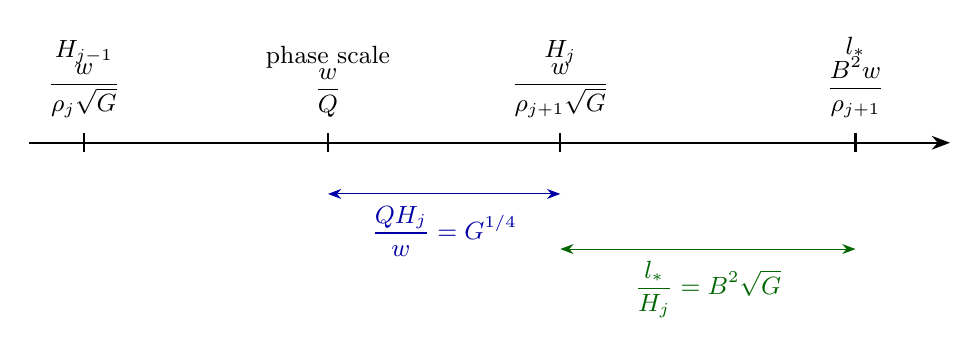
\begin{tikzpicture}[x=1cm,y=1cm,font=\small,>=Stealth]
 \draw[->,thick] (0,0)--(11.7,0);
 \foreach \xx in {.7,3.8,6.75,10.5}
   \draw[thick] (\xx,-.12)--(\xx,.12);
 \node[above,align=center] at (.7,.2)
   {\(H_{j-1}\)\\[-1pt]\(\displaystyle\frac{w}{\rho_j\sqrt G}\)};
 \node[above,align=center] at (3.8,.2)
   {phase scale\\[-1pt]\(\displaystyle\frac{w}{Q}\)};
 \node[above,align=center] at (6.75,.2)
   {\(H_j\)\\[-1pt]\(\displaystyle\frac{w}{\rho_{j+1}\sqrt G}\)};
 \node[above,align=center] at (10.5,.2)
   {\(l_*\)\\[-1pt]\(\displaystyle\frac{B^2w}{\rho_{j+1}}\)};
 \draw[<->,blue!65!black] (3.8,-.65)--(6.75,-.65);
 \node[below,blue!65!black] at (5.275,-.68)
   {\(\displaystyle\frac{QH_j}{w}=G^{1/4}\)};
 \draw[<->,green!40!black] (6.75,-1.35)--(10.5,-1.35);
 \node[below,green!40!black] at (8.625,-1.38)
   {\(\displaystyle\frac{l_*}{H_j}=B^2\sqrt G\)};
\end{tikzpicture}
\caption{The horizontal-length axis (schematic) for a marked block.
Here \(Q=G^{3/4}\rho_{j+1}\) is the retained angular separation and
\(G\rho_{j+1}\le\rho_j\le B\rho_{j+1}\), including the initial block.
The quantity \(l_*=B^2w/\rho_{j+1}\) is the lower bound for predictable
packet lengths in \eqref{hier:predictable-length}.
On an interval of length \(H_j\), the separated relative phases
oscillate many times while the packet envelopes move little.
The preceding mesh also satisfies
\(H_{j-1}\rho_j/w=G^{-1/2}\), which controls the step supremums.
Absolute frequency constants are suppressed.}
\label{fig:phase-scales}
\end{figure}


\subsection{Comparison to the actual factor}

On the underlying real Hilbert space put
\(\mathcal L(Y)=\log(1+\norm Y^p)\). For \(p\ge4\),
\begin{equation}
 \norm{\nabla\mathcal L(Y)}\le p,\qquad
 \norm{D^2\mathcal L(Y)}\le C p^2.
 \label{pred:log-derivatives}
\end{equation}
Indeed its radial first derivative is \(p r^{p-1}/(1+r^p)\),
its radial second derivative is
\[
 \frac{p(p-1)r^{p-2}}{1+r^p}
       -\frac{p^2r^{2p-2}}{(1+r^p)^2},
\]
and each tangential Hessian eigenvalue is
\(p r^{p-2}/(1+r^p)\).
Splitting into \(r\le1\) and \(r\ge1\) proves the bounds; the formulas
extend continuously at zero. No dimension enters these estimates.

If \(\upsilon\ge1/2\), every child was shrunk. The denominator
comparison \eqref{pred:denominator-lower-bound}, the sum of
\eqref{pred:shrunk-numerator-motion}, and
\eqref{pred:log-derivatives} yield
\begin{equation}
 \log\beta_J^0(z)-\log\widetilde\beta(b)
       \le CpK_*\varepsilon\upsilon,\qquad \upsilon\ge1/2.
 \label{pred:balanced-comparison}
\end{equation}
The factor \(\upsilon\) here costs only an absolute factor of two.

For \(0<\upsilon<1/2\), retaining that factor requires the unshrunk
path vector. Write \(\sigma_a=\lambda_a/\abs{\lambda_a}\) and remove
\(\mathcal D_a(b)\) and \(\sigma_a\) from the predicted numerator.
With
\begin{align*}
 Y&=l_a^{1/p}X_a,\\
 C_a&=l_a^{1-\mu-1/p}\abs{\lambda_a}
      =l_a^{1-\alpha/p}(n_a/m_a)^\mu,\\
 Z_1(b)&=\sigma_a^{-1}\mathcal D_a(b)^{-1}
        \sum_{c\ne a}l_c^{1-\mu}\lambda_c
                         \mathcal D_c(b)\widetilde X_c,\\
 R_1&=\sum_{c\ne a}l_c\norm{\widetilde X_c}^p,
\end{align*}
the prediction becomes
\begin{equation}
 \widetilde\beta(b)=
       \frac{1+\norm{C_aY+Z_1(b)}^p}
            {1+\norm Y^p+R_1}.
 \label{pred:path-baseline}
\end{equation}
Here \(Y,C_a\), and the denominator are constant on the whole line.
Since \(n_a\le m_a\le n\), both \(l_a\) and \(n_a/m_a\) lie in
\([1-\upsilon,1]\). As \(1-\alpha/p\ge0\), we have
\begin{equation}
 0<C_a\le1,\qquad 1-C_a\le C\upsilon,\qquad
 \norm{Z_1(b)}\le K_*\upsilon.
 \label{pred:path-coefficient}
\end{equation}

In the actual numerator remove \(\mathcal D_a(b)\) and
\(\sigma_a'=\lambda_a'/\abs{\lambda_a'}\). Define
\[
 Y'=l_a'^{1/p}\mathcal D_a(b)^{-1}X_a',\qquad
 C_a'=l_a'^{1-\mu-1/p}\abs{\lambda_a'},\qquad
 R_1'=\sum_{c\ne a}l_c'\norm{X_c'}^p,
\]
and let \(Z_1'\) be the remaining, similarly rotated off-path sum.
The actual ratio has the form \eqref{pred:path-baseline} with primes.
We have
\begin{align}
 \norm{Y'-Y}&\le C\varepsilon K_*,
 &\abs{C_a'-C_a}&\le C\varepsilon\upsilon,\notag\\
 \norm{Z_1'-Z_1}&\le C\varepsilon K_*\upsilon,
 &R_1'&\ge R_1.
 \label{pred:path-errors}
\end{align}
The first and last statements follow from
\eqref{pred:scaled-motion} and \eqref{pred:denominator-lower-bound}.
For the off-path sum, sum \eqref{pred:shrunk-numerator-motion} over
\(c\ne a\), whose weights sum to at most \(\upsilon\).
Changing the removed scalar phase costs at most \(C\varepsilon\)
times the off-path size, because
\(\abs{\sigma_a'-\sigma_a}\le C\varepsilon\).

The extra \(\upsilon\) in the coefficient estimate follows from the
complementary-mass assertion of \Cref{hier:mass-motion}.
If \(r=A/(A+B)\), with \(A>0\), \(B\ge0\), and the positive
summands change relatively by at most \(C\varepsilon\), then
\[
 |r'-r|\le C\varepsilon r(1-r),\qquad
 |\log r'-\log r|\le C\varepsilon(1-r).
\]
If \(B=0\), the ratio is identically one.
Apply this to \(n_a/n\), with complement \(n-n_a\), and to
\(n_a/m_a\), with complement \(m_a-n_a\).
Both values of \(1-r\) are at most \(\upsilon\).
The bounded nonnegative powers defining \(C_a\) give its claimed
variation. This concerns the modulus of the path weight; its scalar
phase has already been removed.

Set \(\mathfrak r=R_1/(1+\norm Y^p+R_1)\). We claim
\begin{align}
 \log\beta_J^0(z)-\log\widetilde\beta(b)
    &\le C p^2K_*^2\varepsilon\upsilon
           +C pK_*\varepsilon\mathfrak r,\notag\\
 -\log\widetilde\beta(b)
    &\ge \mathfrak r-CpK_*\upsilon.
 \label{eq:src-26}
\end{align}
Hold \(Z_1=Z_1(b)\) fixed when comparing \(Y\) with \(Y'\).
The derivative in \(V\) of
\(\mathcal L(C_aV+Z_1)-\mathcal L(V)\), along that segment, is bounded by
\[
 p|1-C_a|+Cp^2\bigl(|1-C_a|\norm V+\norm{Z_1}\bigr)
       \le Cp^2K_*\upsilon.
\]
Equation~\eqref{pred:path-errors} bounds its change by
\(Cp^2K_*^2\varepsilon\upsilon\).
The changes in \(C_a,Z_1\) fit the same bound by
\eqref{pred:log-derivatives}.

For the residual denominator, set
\[
 J(V)=-\log(1+R_1e^{-\mathcal L(V)}).
\]
Its derivative has norm at most
\(pR_1/(e^{\mathcal L(V)}+R_1)\).
On the segment from \(Y\) to \(Y'\),
\(\abs{\mathcal L(V)-\mathcal L(Y)}\le CpK_*\varepsilon\).
This tends to zero as \(L\) increases, so that residual ratio is at
most \(2\mathfrak r\), and
\(J(Y')-J(Y)\le CpK_*\varepsilon\mathfrak r\).
The actual residual \(R_1'\ge R_1\) can only decrease the actual
ratio. This proves the first inequality of \eqref{eq:src-26}.
For the second, use \(C_a\le1\), \eqref{pred:log-derivatives},
and \(\log(1+t)\ge t/(1+t)\):
\begin{align*}
 -\log\widetilde\beta
 &=\mathcal L(Y)-\mathcal L(C_aY+Z_1)
       +\log(1+R_1e^{-\mathcal L(Y)})\\
 &\ge-p\norm{Z_1}+\mathfrak r
 \ge\mathfrak r-CpK_*\upsilon.
\end{align*}

\subsection{Absorbing the baseline error by blending}

The parameter sizes give
\begin{equation}
 pK_* = G^{o(1)}\quad\text{as }L\longrightarrow\infty,
 \label{pred:subpower-amplitude}
\end{equation}
with every preceding constant fixed.
Indeed \(\log N\le2L\), \(\mu=O(L^{-1/2})\), and
\(\log G\asymp L^{7/10}\), so
\(\log(pK_*)=O(\sqrt L+\log L)=o(\log G)\).
All the preceding smallness requirements consequently follow from a
single sufficiently large lower bound on \(L\).

Set \(\theta_{\mathrm{bl}}=\sqrt\varepsilon\) and blend the prediction with one:
\begin{equation}
 \mathcal B(b)=(1-\theta_{\mathrm{bl}})\widetilde\beta(b)+\theta_{\mathrm{bl}}.
 \label{pred:blend}
\end{equation}
It retains average at most one for every probability in
\Cref{pred:fourier-average}. Concavity of the logarithm gives
\[
 \log \mathcal B-\log\widetilde\beta
       \ge-\theta_{\mathrm{bl}}\log\widetilde\beta.
\]
For \(\upsilon<1/2\), Equation~\eqref{eq:src-26} yields
\begin{align*}
 \log\beta_J^0-\log \mathcal B
 &\le\bigl(Cp^2K_*^2\varepsilon+CpK_*\theta_{\mathrm{bl}}\bigr)\upsilon
       +\bigl(CpK_*\varepsilon-\theta_{\mathrm{bl}}\bigr)\mathfrak r\\
 &\le\bigl(Cp^2K_*^2\varepsilon
                  +CpK_*\sqrt\varepsilon\bigr)\upsilon.
\end{align*}
The last coefficient of \(\mathfrak r\) is nonpositive for large \(L\).
For \(\upsilon\ge1/2\), use \eqref{pred:balanced-comparison} and
\(\log\widetilde\beta\le\mathcal L(F)\le p\norm F\le CpK_*\)
to obtain the same last bound. Therefore
\begin{equation}
 \beta_J^0(z)\le e^{a_L\upsilon}\mathcal B(b),\qquad
 a_L=Cp^2K_*^2\varepsilon+CpK_*\sqrt\varepsilon
       \le G^{-\gamma/3}
 \label{pred:blended-domination}
\end{equation}
for sufficiently large \(L\).
The baseline has absorbed the term proportional to \(\mathfrak r\);
the remaining error is proportional to \(\upsilon\).

\subsection{Changing to uniform measure without a loss per level}

Choose a fixed nonnegative Schwartz function \(k\) of integral one
with \(\supp\widehat k\subset[-1/4,1/4]\).
For example, square the absolute value of the inverse Fourier
transform of a nonzero smooth function supported in \((-1/8,1/8)\)
and normalize its integral.
Let \(H=H_j\), \(h=G^{-1/16}\), \(s=HG^{-1/8}\), and
\(k_s(t)=s^{-1}k(t/s)\).
Let \(I^+\) be the concentric enlargement of \(I\) of length
\((1+h)H\), and define
\begin{equation}
 \dd\nu_I(t)=
      \left(\frac{\one_{I^+}}{|I^+|}*k_s\right)(t)\,\dd t.
 \label{pred:majorant-probability}
\end{equation}
This is a positive probability whose Fourier transform is supported
in \([-1/(4s),1/(4s)]\).
Since \(H\delta=\epsilon'G^{1/4}\), this support lies strictly inside
\((-\delta,\delta)\) for large \(L\).

Every point of \(I\) is at distance at least \(hH/2\) from the
complement of \(I^+\). The Schwartz tail beyond
\((hH)/(2s)=G^{1/16}/2\) is \(O(G^{-1/8})\), by a fixed tail estimate.
Thus the density in \eqref{pred:majorant-probability} is at least
\(H^{-1}(1-CG^{-1/16})\) on \(I\).
Writing \(\omega_I\) for uniform probability on \(I\), choose
\(0<\eta\le CG^{-1/16}<1/2\) so that
\begin{equation}
 \nu_I\ge(1-\eta)\omega_I,\qquad
 \nu_I=(1-\eta)\omega_I+\eta\nu_{\rm rem}
 \label{pred:measure-decomposition}
\end{equation}
for a positive probability \(\nu_{\rm rem}\).

The bound \(\int \mathcal B\,\dd\nu_I\le1\) alone would lose an amount of
order \(\eta\) on changing measure. We need a bound proportional to
\(\upsilon\).
If \(\widetilde\beta\le1\) on the whole line, then \(\mathcal B\le1\) and
its uniform average is already at most one.
Otherwise choose \(b_0\) with \(\widetilde\beta(b_0)>1\).
When \(\upsilon<1/2\), the denominator and path vector in
\eqref{pred:path-baseline} are fixed. For all \(b\in\R\),
\begin{align*}
 \log\widetilde\beta(b)
 &\ge\log\widetilde\beta(b_0)
          -p\norm{Z_1(b)-Z_1(b_0)}\\
 &\ge-2pK_*\upsilon.
\end{align*}
Consequently
\begin{equation}
 (1-\widetilde\beta(b))_+\le CpK_*\upsilon
       \qquad(b\in\R).
 \label{pred:negative-deviation}
\end{equation}
This does not assume an upper bound on \(R_1\): its contribution
cancels in the logarithmic difference. Equivalently, a value exceeding
one already forces
\(R_1/(1+\norm Y^p)\le e^{CpK_*\upsilon}-1\).
For \(\upsilon\ge1/2\), Equation~\eqref{pred:negative-deviation}
follows from nonnegativity since \(pK_*\upsilon\ge1\).
The blend inherits the same lower bound, as
\((1-\mathcal B)_+=(1-\theta_{\mathrm{bl}})(1-\widetilde\beta)_+\).

In the case where the prediction exceeds one somewhere,
\eqref{pred:measure-decomposition} gives
\[
 1\ge\int \mathcal B\,\dd\nu_I
 \ge(1-\eta)\int \mathcal B\,\dd\omega_I
           +\eta(1-CpK_*\upsilon).
\]
Including the easier case \(\mathcal B\le1\), this proves
\begin{equation}
 \int \mathcal B\,\dd\omega_I\le1+C G^{-1/16}pK_*\upsilon.
 \label{pred:uniform-average}
\end{equation}
The relative mass drop has survived the change of probability.

\subsection{Step supremums and normalization}

The points \(s_R,t_c\) lie in \(J\), so all component frequencies
of \(\mathcal D_c\) have magnitude at most \(C\rho_j/w\).
For \(\upsilon\ge1/2\), differentiating \eqref{pred:model} and using
\eqref{pred:snapshot-size} gives
\(\norm{\partial_b F(b)}\le C(\rho_j/w)K_*\).
For \(\upsilon<1/2\), remove the path carrier as in
\eqref{pred:path-baseline}. The off-path frequencies are
\((t_a-t_c)\eta_\xi\), again of magnitude at most \(C\rho_j/w\), so
\(\norm{\partial_b Z_1(b)}\le C(\rho_j/w)K_*\upsilon\).
In both cases,
\[
 \left|\frac{\dd}{\dd b}\log\widetilde\beta(b)\right|
       \le CpK_*\upsilon\frac{\rho_j}{w}.
\]
Blending cannot increase the absolute logarithmic derivative, because
\[
 \frac{\dd}{\dd b}\log \mathcal B
   =\frac{(1-\theta_{\mathrm{bl}})\widetilde\beta}{\mathcal B}
               \frac{\dd}{\dd b}\log\widetilde\beta,\qquad
 0\le\frac{(1-\theta_{\mathrm{bl}})\widetilde\beta}{\mathcal B}\le1.
\]

On each \(H_{j-1}\)-subcell \(I'\subset I\), let \(\mathcal B^\sharp\) equal
\(\sup_{b\in\overline{I'}}\mathcal B(b)\).
The prediction is positive and continuous, and these compact-cell
supremums are finite. The meshes are nested. Since
\(H_{j-1}\rho_j/w=G^{-1/2}\),
\begin{equation}
 \mathcal B\le \mathcal B^\sharp\le e^{b_L\upsilon}\mathcal B,\qquad
 b_L=CpK_*G^{-1/2}.
 \label{pred:step-supremum}
\end{equation}
Use the fixed half-open mesh convention at endpoints; taking
supremums over closed subcells preserves the inequalities.
Define
\begin{equation}
 m_I=\max\left(1,\int \mathcal B^\sharp\,\dd\omega_I\right),\qquad
 \Gamma_j=\mathcal B^\sharp/m_I\quad\text{on }I.
 \label{pred:gamma-normalization}
\end{equation}
This function is nonnegative, constant on the finer cells, and has
average at most one. Equations~\eqref{pred:uniform-average} and
\eqref{pred:step-supremum} yield
\begin{equation}
 \log m_I\le\bigl(b_L+CG^{-1/16}pK_*\bigr)\upsilon.
 \label{pred:normalization-cost}
\end{equation}

\begin{proof}[Proof of \Cref{pred:marked-comparison}]
Perform the construction on each marked cell meeting \(Z\).
Equations~\eqref{pred:blended-domination},
\eqref{pred:step-supremum}, and \eqref{pred:gamma-normalization} give
\[
 \beta_J^0(z)\le e^{a_L\upsilon}\mathcal B(b)
       \le e^{a_L\upsilon}\mathcal B^\sharp(b)
       =e^{a_L\upsilon}m_I\Gamma_j(b).
\]
By \eqref{pred:normalization-cost}, the exponent is at most
\[
 \bigl(G^{-\gamma/3}+CpK_*G^{-1/2}
                    +CpK_*G^{-1/16}\bigr)\upsilon.
\]
Equations~\eqref{pred:subpower-amplitude} and
\eqref{pred:drop-comparability} bound this by
\(G^{-c_{\rm av}}u_j(z)\), for a fixed positive exponent:
choose \(c_{\rm av}<\min(\gamma/4,1/64)\) and then take \(L\)
sufficiently large. This proves \eqref{eq:src-24} with no error
independent of the mass drop.

There are countably many cells on each fixed line and finitely many
levels in the current truncation. Choose one snapshot in every
relevant cell, use \eqref{pred:gamma-normalization} there, and set
\(\Gamma_j=1\) elsewhere. This is a measurable step function of the
line parameter. The proof of \Cref{res:path-product} integrates the
original integrand on lines where its slice is measurable, as holds for
almost every transverse parameter. It therefore needs no jointly
measurable snapshot choices across parallel lines.
\end{proof}

\section{Residual terms and integration along paths}
\label{res:section}

We work with a finite tile collection and a fixed angular translation.
Fix a shift $\sigma$ and a parameter $\zeta$ whose real part is the
corresponding vertex: $\Re\zeta_\sigma=\mu$, all other real parts vanish,
and $\norm{\Im\zeta}_2\le L^2$.  All estimates in this section are
uniform in these choices, the number of tiles, the angular depth, and
$\dim\mathcal H$.  We take $L$ sufficiently large that
\begin{equation}
  p>\alpha,\qquad 0<\mu\le\frac1{12}.
  \label{res:small-mu}
\end{equation}
We retain the stopping threshold $M=L^{A_M}$ from
\eqref{hier:mass-cutoff}; its fixed exponent will be chosen at the end
of the residual estimates.

Fix a path top $R$.  We retain the block notation of the hierarchy:
$J_j=v_{i_j}(R)$, $n_j=n_{J_j}$, and $A_j=A_{J_j}$.
The last possible block is the last one whose starting node contains
$R$ as an eligible top.  At this last block there is no path child,
even if other tops continue; the next path mass is defined to be zero.
At every other block write $J_{j+1}$ for the path child and set
\[
  h_j^*=n_j-n_{j+1},\qquad u_j=\frac{h_j^*}{n_j}.
\]
An index is active if $n_j>M$.  The active indices form a prefix.
On $Z$, the mass bound \eqref{eq:src-12} and monotonicity give
\begin{equation}
  \sum_{j\text{ active}}u_j\le C L.
  \label{res:relative-drop-sum}
\end{equation}
Indeed, except for the last active index, use
$1-n_{j+1}/n_j\le\log(n_j/n_{j+1})$ and telescope down to a mass
larger than $M$.  The final summand is at most one.  This proof also
applies when the path stops by ineligibility.

\subsection{Marked residuals}

For $n>0$ and $A\in\mathcal H$, put
\[
  V(n,A)=n+n^{\alpha-p}\norm{A}^{p}
        =n\bigl(1+\norm{n^{\mu-1}A}^{p}\bigr).
\]
The function $\mathcal L_p(Y)=\log(1+\norm{Y}^{p})$ is globally
$p$-Lipschitz on the underlying real Hilbert space.  Away from zero
its derivative has norm
$p\norm{Y}^{p-1}/(1+\norm{Y}^{p})\le p$, and the assertion at zero
follows by continuity.  Since $\beta_J$ and $\beta_J^0$ have the same
denominator, the decomposition \eqref{eq:src-18} therefore implies
\begin{equation}
  \log\beta_{J_j}-\log\beta_{J_j}^0
       \le Cp\,n_j^{-1+\mu}\norm{B_{J_j}}.
  \label{eq:src-27}
\end{equation}

\begin{lemma}[Square summation of residual blocks]
\label{res:block-square}
At a point $z\in Z$ where $R$ is a good path,
\begin{equation}
  \left(\sum_j\norm{B_{J_j}(z)}^2\right)^{1/2}\le L^{C_b}.
  \label{res:block-square-bound}
\end{equation}
Here the sum can be restricted to any subset of the possible blocks.
The fixed exponent $C_b$ is independent of $M$.
\end{lemma}

\begin{proof}
A residual packet in block $j$ has
\begin{equation}
  \frac{\rho_{j+1}}{B^2}<d_s\le\frac{\rho_j}{B^2},
  \qquad i_j\le k_s<i_{j+1}.
  \label{res:residual-range}
\end{equation}
Because $\rho_j/\rho_{j+1}\le B$, this block contains at most
$N_{\mathrm{len}}:=C(1+\log B)$ dyadic packet lengths.  Also $s_{T(s)},s_R\in J_j$,
so the top assignment and \eqref{res:residual-range} imply
\[
  \abs{\theta_s-s_R}
     \le C d_s+\rho_j
     \le C B^3 d_s\le C B^4d_s.
\]
Thus the reference-line estimates apply whenever $\ell_s\le l_R$.

The coefficient multiplying $q_{T(s)}\phi_s$ in $B_{J_j}$ is a
product of transition weights of modulus at most one, followed by
$n_{v_{k_s}(T(s))}^{-\mu/K}$.  The ending mass is at least
$h_{T(s)}$.  Consequently the modulus of the coefficient multiplying
$\phi_s$ is at most
$|q_{T(s)}|h_{T(s)}^{-\mu/K}\le C$.  This last bound follows from
the mask estimate \eqref{eq:src-8}: on the significant region
$h_T\ge1$, while off that region the mask has faster decay than
this fixed small negative power of $h_T$.

At $z$ let $e_\ell$ and $a_\ell$ be the sums of the absolute error and
main envelopes, respectively, at length $\ell$ in the fixed family
$\mathcal P_R$ of \eqref{hier:reference-packets}.  The preceding bounds
place every residual packet with $\ell_s\le l_R$ in this family, so its
absolute envelopes are included in these positive sums.  Goodness of $R$,
as specified in \Cref{hier:good-paths}, gives
\[
  \sum_{\ell\le l_R}e_\ell\le L^C,
  \qquad
  \left(\sum_{\ell\le l_R}a_\ell^2\right)^{1/2}\le L^C.
\]
The contribution of such lengths to $\norm{B_{J_j}}$ is bounded by
$C\sum_{\ell\in\mathcal I_j}(e_\ell+a_\ell)$, where
$\mathcal I_j$ is the set of residual lengths in that block.
The sets $\mathcal I_j$ are disjoint.  Positivity and
Cauchy--Schwarz within each block therefore give
\begin{align*}
 \left\{\sum_j
    \left(\sum_{\ell\in\mathcal I_j,\,\ell\le l_R}
                         e_\ell\right)^2\right\}^{1/2}
       &\le\sum_{\ell\le l_R}e_\ell,\\
 \sum_j\left(\sum_{\ell\in\mathcal I_j,\,\ell\le l_R}
                         a_\ell\right)^2
       &\le N_{\mathrm{len}}\sum_{\ell\le l_R}a_\ell^2.
\end{align*}
The factor $N_{\mathrm{len}}$ is polynomial in $L$.

Before the last possible block, $R$ remains eligible at the child
level.  Hence $d_R\le\rho_{j+1}/B^2<d_s$, and consequently
$\ell_s<l_R$.  Lengths larger than $l_R$ can occur only in the last
possible block.  At each of its at most $N_{\mathrm{len}}$ lengths, the total
absolute coefficient envelope is bounded by a constant, by
\Cref{conc:single-scale}, applied with reference length equal to
that scale.  To recall the reason this bound has no
factor counting the available labels, the condition
$|\theta_s-s_R|\le CB^4d_s$ makes the analyzing and synthesizing
box envelopes comparable to common $s_R$-coordinate envelopes, since
$W\gg B^4w$.  Summing centers first produces a common positive
convolution kernel of integral $O(1)$.  At each source point only
boundedly many selector labels are nonzero.  Summing these labels
then uses $\norm{g}_{\mathcal H}\le1$, and costs $O(1)$.
The uniformly bounded multipliers just considered preserve this
absolute estimate.  The last block therefore contributes at most
$C N_{\mathrm{len}}$ in norm.  Combining the estimates proves
\eqref{res:block-square-bound}.
\end{proof}

By \Cref{hier:marking}, at any marked point one has $h_j^*\ge c_m$
for a fixed $c_m>0$.  Monotonicity of the masses therefore implies
\begin{equation}
  \#\{j:\ j\text{ marked at }z,\ t\le n_j<2t\}
         \le C(1+t),\qquad t\ge M.
  \label{res:marked-shell-count}
\end{equation}
For completeness, all but the final marked index in this shell
account for disjoint mass drops of size at least $c_m$ while the mass
lies in an interval of length at most $t$; the final index costs one
even if its drop leaves the shell.  Dyadic summation gives
\begin{equation}
 \sum_{j\text{ marked at }z}n_j^{-2+2\mu}
       \le C\sum_{r\ge0}(2^rM)^{-1+2\mu}
       \le C M^{-1+2\mu}.
 \label{res:marked-weight-sum}
\end{equation}
Combining \eqref{eq:src-27}, \Cref{res:block-square}, and
Cauchy--Schwarz yields
\begin{equation}
 \sum_{j\text{ marked at }z}
       \bigl(\log\beta_{J_j}-\log\beta_{J_j}^0\bigr)
       \le CpL^{C_b}M^{-1/2+\mu}.
 \label{res:marked-cost}
\end{equation}

\subsection{Unary segments and their energy telescope}

Call an active index \emph{unary} at $z$ if its cell is unmarked and
$h_j^*(z)<1$.  At such an index the path child exists: at the last
possible block the drop would instead be $n_j>M$.  A significant top
has mass at least one.  Thus every significant top eligible in $J_j$
must remain eligible in the path child, since the total mass removed
from that child is $h_j^*<1$.

At a unary index write
\begin{equation}
  A_j=\lambda_j A_{j+1}+U_j+W_j.
  \label{res:unary-decomposition}
\end{equation}
Here $\lambda_j$ is the path-child coefficient in
\eqref{eq:src-18}; $U_j$ consists of the residual packets assigned
to tops which remain eligible in the path child.  These are exactly
the packets of the fixed subset $\mathcal Q_{R,\sigma}$ in
\eqref{hier:deterministic-residual-subset} which stop in block $j$.  The term $W_j$
collects all contributions of tops eligible in $J_j$ which do not
continue in the path child, including their residual packets and,
when present, their contributions through other children.

Those latter tops are all insignificant at $z$.  Their contributions
within $A_{J_j}$ are whole interval sums on individual tops, so
\Cref{hier:amplitudes} bounds the contribution of each by
$L^C(1+\norm{\zeta})|q_T|h_T^4$.  Since $h_T$ is bounded above by
an absolute constant and $|q_T|\le e^{-L\log L}$ there, this is at
most $Ce^{-L}h_T$ for sufficiently large $L$.  The masses of these
tops sum to $h_j^*$.  Therefore
\begin{equation}
  \norm{W_j}\le Ce^{-L}h_j^*.
  \label{res:discarded-top-error}
\end{equation}
This estimate uses a sum of top masses, not the number of such tops.

Partition each consecutive run of unary indices into consecutive
segments $[e,f)$.  Starting at $e$, end a completed segment as soon
as its accumulated drop is at least one.  Each individual drop is
less than one, so every completed segment has total drop in $[1,2)$.
At the end of the run, retain the final remainder as one segment if
it is nonempty.  Hence every segment satisfies
\begin{equation}
  \Delta_{e,f}:=\sum_{e\le j<f}h_j^*=n_e-n_f<2,
  \qquad n_f>M-2,
  \qquad n_j\asymp n_e\quad(e\le j\le f).
  \label{res:segment-masses}
\end{equation}
The endpoint remains an eligible path node, including when it is the
node where the mass stopping rule first applies.

The number of segment starts in a mass shell obeys
\begin{equation}
  \#\{[e,f):\ t\le n_e<2t\}\le C(1+t),\qquad t\ge M.
  \label{res:segment-shell-count}
\end{equation}
Completed segments account for disjoint drops of size at least one.
For each remainder other than the final remainder on the path,
charge it to the next interruption of a unary run.  Such an
interruption is either marked, with drop at least $c_m$, or is an
active unmarked index with drop at least one.  The mass at this
interruption differs from the start mass of the remainder by less
than two.  Thus the interruptions charged by starts in $[t,2t)$
lie in the enlarged shell $[t-2,2t)$ and their fixed positive drops
give $O(1+t)$ choices.  The one possible final remainder adds one.

For one segment define
\[
 A_i^*=\left(\prod_{i\le j<f}\lambda_j\right)A_f,
 \qquad V_i^*=V(n_i,A_i^*),\qquad e\le i\le f,
\]
with the empty product equal to one.  Since $n_i\ge n_{i+1}$,
$\alpha-p<0$, and $|\lambda_i|\le1$, we have
\begin{equation}
  V_i^*\le h_i^*+V_{i+1}^*,\qquad V_f^*=V_f.
  \label{res:starred-subsolution}
\end{equation}
Indeed, the baseline terms differ by $h_i^*$, while the energy
term on the left is at most
$n_{i+1}^{\alpha-p}\norm{A_{i+1}^*}^p$.
The denominator of $\beta_{J_i}$ contains the energy of the path
child and the nonnegative energies of all other children.  It is
therefore at least $h_i^*+V_{i+1}$.  It follows that
\[
 \sum_{e\le i<f}\log\beta_{J_i}
 \le \log V_e-\log V_f
       -\sum_{e\le i<f}\log(1+h_i^*/V_{i+1}).
\]
On the other hand, \eqref{res:starred-subsolution} gives
\[
 \log V_e^*-\log V_f
       \le\sum_{e\le i<f}\log(1+h_i^*/V_{i+1}^*).
\]
Subtracting these inequalities produces the useful estimate
\begin{equation}
 \begin{aligned}
 \sum_{e\le i<f}\log\beta_{J_i}
 &\le \log(V_e/V_e^*)
       +\sum_{e\le i<f}
           \left[\log(1+h_i^*/V_{i+1}^*)
                 -\log(1+h_i^*/V_{i+1})\right] \\
 &\le Cp\, n_e^{-1+\mu}
            \max_{e\le i\le f}\norm{A_i-A_i^*}.
 \end{aligned}
 \label{eq:src-28}
\end{equation}
To justify the last line, first use the Lipschitz estimate for
$\mathcal L_p$ to obtain
\[
  |\log V(n,A)-\log V(n,A')|
       \le p n^{\mu-1}\norm{A-A'}.
\]
For $h\ge0$, the derivative of $x\mapsto\log(1+he^{-x})$ has
absolute value $h/(e^x+h)$.  Along the interval between
$\log V_{i+1}$ and $\log V_{i+1}^*$, both endpoint amounts, and
therefore every intermediate amount, are at least $n_{i+1}$.
The corresponding correction term is bounded by
\[
 \frac{h_i^*}{n_{i+1}}
      p n_{i+1}^{\mu-1}\norm{A_{i+1}-A_{i+1}^*}.
\]
Now use \eqref{res:segment-masses} and
$\sum_{e\le i<f}h_i^*/n_{i+1}\le2/(M-2)$.  This proves
\eqref{eq:src-28}, including its endpoint case.

\subsection{Common residual weights and variation}

We give the coefficient calculation needed to apply the good-path
variation estimate.  It is important here that the same angular
grid underlies all shifts.

For integer levels $k$ along the path put
$v_k=v_k(R)$ and $a_k=n_{v_k}$, so $a_{i_j}=n_j$.
For a fixed segment $[e,f)$ and a block index $j\in[e,f)$, define
\begin{equation}
 \omega_j(k)=a_k^{-\mu/K}
     \prod_{r=i_j}^{k-1}
       \left(\frac{a_{r+1}}{m_{v_{r+1}}}\right)^{\zeta_{r\bmod K}},
 \qquad i_j\le k<i_f.
 \label{res:common-weight}
\end{equation}
Here $i_j$ denotes the angular level at the start of block $j$.

Every packet in $U_b$, for $j\le b<f$, is assigned to a top in
$v_{i_{b+1}}(R)$.  It follows by nesting that its top lies in $v_k(R)$
at every intermediate level $k\le i_{b+1}$, in particular at its
stopping level $k_s$.  Multiplying its coefficient in $U_b$ by the
path propagation factor $\prod_{j\le r<b}\lambda_r$ therefore
gives exactly $\omega_j(k_s)q_{T(s)}\phi_s$.
This identity holds for every contributing top, whether or not that
top is significant.  Thus the scalar coefficient depends only on
the stopping level, rather than on the packet or top inside that
level.

\begin{lemma}[Variation of the common coefficients]
\label{res:common-weight-variation}
Uniformly over the segments and their starting indices,
\begin{equation}
  \sup_{i_j\le k<i_f}|\omega_j(k)|
    +\sum_{k=i_j}^{i_f-2}|\omega_j(k+1)-\omega_j(k)|
       \le L^{C_w}.
  \label{res:common-weight-BV}
\end{equation}
The exponent $C_w$ is fixed before $M$ is chosen.
\end{lemma}

\begin{proof}
Every ending mass in this sequence is at least
$a_{i_f}=n_f>M-2$.  Since all real parts of $\zeta$ are nonnegative,
$|\omega_j(k)|\le a_k^{-\mu/K}\le1$ when $M\ge3$.
Using the real logarithms of positive masses, a logarithmic
increment of the coefficient is
\[
 \log\omega_j(k+1)-\log\omega_j(k)
 =\frac{\mu}{K}\log\frac{a_k}{a_{k+1}}
     -\zeta_{k\bmod K}\log\frac{m_{v_{k+1}}}{a_{k+1}}.
\]
The logarithm here is the specified linear expression defining the
coefficient, so no branch of a complex logarithm is being chosen.
The first sum of absolute increments telescopes.  For the second
use \Cref{hier:weight-variation} on the entire root-to-endpoint
path.  All its summands are nonnegative, whence
\begin{align*}
 \sum_{k=i_j}^{i_f-2}
    |\log\omega_j(k+1)-\log\omega_j(k)|
 &\le \left(\frac{\mu}{K}
          +K\max_\sigma|\zeta_\sigma|\right)
            \log\frac{n_{\mathrm{root}}}{n_f} \\
 &\le L^{C_w}.
\end{align*}
The last step uses $n_{\mathrm{root}}\le NL^C$ on $Z$,
$\log N\le2L$, $n_f> M-2\ge1$, and
$\max_\sigma|\zeta_\sigma|\le\mu+L^2$.
The full-root bound is needed: a denominator $m_v$ belonging to a
different shift may involve a block whose starting level precedes
the segment.  No estimate using only $\log(n_e/n_f)$ is asserted.

For two successive logarithmic values $z_0,z_1$ in this sequence,
both $|e^{z_0}|$ and $|e^{z_1}|$ are at most one.  Along the straight
segment between them, $|e^{(1-t)z_0+tz_1}|\le1$.  Integration of
the derivative of the exponential consequently yields
$|e^{z_1}-e^{z_0}|\le|z_1-z_0|$.
The logarithmic-increment bound proves
\eqref{res:common-weight-BV}.
\end{proof}

Let $\mathcal Q_{R,\sigma}$ denote the fixed residual subset in
\eqref{hier:deterministic-residual-subset}.  For each unary segment $[e,f)$ define
\[
 \Lambda_{e,f}(z)=
    \max_{i_e\le a\le b<i_f}
       \left\|\sum_{\substack{s\in\mathcal Q_{R,\sigma}\\
                              a\le k_s\le b}}
                       q_{T(s)}(z)\phi_s(z)\right\|.
\]
An empty sum has value zero.  Finite depth makes the maximum finite.
The interval of stopping levels $[a,b]$ corresponds to an interval
of dyadic packet lengths.  The latter follows directly from the
definition $k_s=\max\{k:d_s\le d(k)/B^2\}$, which is monotone
in $\ell_s$.  Since distinct unary segments have disjoint level
intervals $[i_e,i_f)$, one may choose a maximizing interval in each
segment and apply the single good-path $3$-variation bound to all
those disjoint intervals.  Thus
\begin{equation}
  \left(\sum_{[e,f)}\Lambda_{e,f}(z)^3\right)^{1/3}
       \le L^{C_v}.
  \label{res:segment-cube-sum}
\end{equation}
The segments may depend on $z$; the variation is a supremum over
all choices of disjoint intervals, so this dependence does not
alter the inequality.  The underlying packet subset itself is the
single deterministic set $\mathcal Q_{R,\sigma}$.

Abel summation for a finite scalar sequence $(\omega_k)$ and vector
sequence $(F_k)$ gives
\[
 \left\|\sum_{k=a}^b\omega_k F_k\right\|
 \le \left(|\omega_b|+
             \sum_{k=a}^{b-1}|\omega_k-\omega_{k+1}|\right)
                \max_{a\le t\le b}
                       \left\|\sum_{k=a}^tF_k\right\|.
\]
Applying this identity with \eqref{res:common-weight}, and then
iterating \eqref{res:unary-decomposition}, yields
\begin{equation}
 \max_{e\le i\le f}\norm{A_i-A_i^*}
    \le L^{C_w}\Lambda_{e,f}
           +Ce^{-L}\Delta_{e,f}.
 \label{res:segment-perturbation}
\end{equation}
Indeed the propagated $W_j$ terms have modulus at most their
unpropagated bounds because $|\lambda_j|\le1$.
There are no residual terms beyond $i_f$ in this calculation:
$U_j$ uses only $i_j\le k_s<i_{j+1}$ with $j<f$.
When $f$ is a mass-stopping node it is still an eligible node and
\eqref{res:segment-masses} applies.  A final block ending by
ineligibility cannot be unary and is excluded from this calculation.

Using \eqref{res:segment-shell-count} and dyadic mass shells, we get
\begin{equation}
 \begin{split}
 \sum_{[e,f)}n_e^{(-1+\mu)3/2}
   &\le C\sum_{r\ge0}(2^rM)^{-1/2+3\mu/2}
    \le C M^{-1/2+3\mu/2},\\
 \left(\sum_{[e,f)}n_e^{(-1+\mu)3/2}\right)^{2/3}
   &\le C M^{-1/3+\mu}.
 \end{split}
 \label{res:segment-weight-sum}
\end{equation}
H\"older with exponents $3/2$ and $3$, followed by
\eqref{eq:src-28}, \eqref{res:segment-cube-sum}, and
\eqref{res:segment-perturbation}, therefore bounds the sum of the
unary log factors by
\begin{equation}
 \sum_{j\text{ unary at }z}\log\beta_{J_j}
       \le CpL^{C_u}M^{-1/3+\mu}
          +Cp e^{-L}\left(\max_{j\text{ active}}n_j^\mu\right)
                              \sum_{j\text{ active}}u_j.
 \label{res:unary-cost}
\end{equation}
For the error term, use $n_e\ge n_j$ and $\mu-1<0$ within a
segment to obtain
$n_e^{\mu-1}h_j^*\le n_j^{\mu-1}h_j^*=n_j^\mu u_j$.
By \eqref{eq:src-12}, $\max n_j^\mu\le\exp(C\sqrt L)$.
Together with \eqref{res:relative-drop-sum}, this makes the second
term in \eqref{res:unary-cost} tend to zero.

Choose a fixed exponent $C_{\mathrm{res}}$ larger than all polynomial
exponents in \eqref{res:marked-cost} and \eqref{res:unary-cost},
and then choose
\begin{equation}
  A_M>4(C_{\mathrm{res}}+2),\qquad M=L^{A_M}.
  \label{res:choice-M}
\end{equation}
By \eqref{res:small-mu}, $-1/3+\mu\le-1/4$ and
$-1/2+\mu\le-5/12$.  Since $p=L^{1/2}$, this choice makes both
principal residual costs bounded by an absolute constant for
sufficiently large $L$.  None of the good-path thresholds or the
exponents used to select $A_M$ depended on $M$.

\subsection{The path product and its integral}

\begin{theorem}[Integrated path product]
\label{res:path-product}
With $M$ chosen by \eqref{res:choice-M}, the estimate
\eqref{eq:src-22} holds for every path top $R$, every shift, and
every vertex parameter with $\norm{\Im\zeta}_2\le L^2$.
Its constants are independent of the tile collection, angular
depth, and Hilbert-space dimension.
\end{theorem}

\begin{proof}
Fix a line of slope $s_R$, and on that line use the functions
$\Gamma_j$ constructed in \Cref{pred:marked-comparison}.
At a point of $Z$ where $R$ is good, the active indices fall into
the marked indices, the unary indices, and at most one active
unmarked index with $h_j^*\ge1$.
For the marked indices, combine \eqref{eq:src-24},
\eqref{res:marked-cost}, and
\eqref{res:relative-drop-sum}.  Their phase-domination losses have
sum at most $CLG^{-c}$, which is bounded.  The unary factors have
bounded log product by \eqref{res:unary-cost} and
\eqref{res:choice-M}.

At the possible remaining index, \Cref{hier:marking} gives
$M<n_j<M+1$.  From \eqref{eq:src-17} and the baseline $n_j$ in
the denominator of $\beta_{J_j}$,
\[
  \beta_{J_j}\le 1+L^{Cp}n_j^{\alpha-1}
       \le L^{Cp}(1+M)^C.
\]
Here $C$ is fixed, since $\alpha$ stays in a fixed compact interval
below three.  We have therefore proved the pointwise domination
\begin{equation}
 \prod_{j\text{ active at }z}\beta_{J_j}(z)
       \le L^{Cp}(1+M)^C\prod_{j=0}^{J_R}\Gamma_j(z),
 \qquad z\in Z\cap\{R\text{ good}\},
 \label{res:pointwise-product}
\end{equation}
where $J_R$ is the last possible block index for $R$.
It is legitimate to include every possible index on the right:
if $n_j(z)\le M$, its mesh cell cannot satisfy
$\inf n_j>M$, so it is unmarked and $\Gamma_j(z)=1$.
Unmarked active indices likewise have $\Gamma_j=1$.

Recall that $\Gamma_j$ is constant on the mesh of length $H_{j-1}$
and has average at most one on every cell of length $H_j$.
The meshes are nested.  On any cell $I$ of the largest mesh
$H_{J_R}$, successive averaging from the smallest mesh upward
therefore gives
\begin{equation}
  \int_I\prod_{j=0}^{J_R}\Gamma_j(x)\,\dd x\le |I|.
  \label{res:mesh-average}
\end{equation}
More explicitly, all later factors $\Gamma_k$, $k>j$, are constant
on each $H_j$ cell.  Integrating $\Gamma_j$ on those cells can thus
only decrease the integral of the nonnegative product.  Iterate
this observation for $j=0,1,\ldots,J_R$.

The weight $h_R$ is uniformly comparable on $I$.  This remains true
for a terminal block and for the short first block: eligibility
of $R$ at $i_j$ gives $\rho_j\ge B^2d_R$, and every block has
$\rho_j/\rho_{j+1}\le B$.  Thus
\begin{equation}
  H_j=\frac{w}{\rho_{j+1}\sqrt G}
        \le\frac{l_R}{B\sqrt G}\le l_R.
  \label{res:mesh-versus-top}
\end{equation}
Along the line of slope $s_R$, the transverse normalized coordinate
of $R$ is fixed and the horizontal normalized coordinate changes
by at most $H_j/l_R$.  The definition \eqref{eq:src-5} consequently
gives $\sup_I h_R\le C\inf_Ih_R$, with an absolute constant
depending only on the fixed decay exponent.  By
\eqref{res:mesh-average},
\[
 \int_I h_R\prod_{j=0}^{J_R}\Gamma_j\,\dd x
     \le (\sup_Ih_R)|I|\le C\int_Ih_R\,\dd x.
\]
Sum over the largest-mesh cells and use
\eqref{res:pointwise-product}.  Whenever the original integrand in
\eqref{eq:src-22} has a measurable slice on this line, we obtain
\[
 \int_{Z\cap\{R\text{ good}\}\text{ on the line}}
       h_R\prod_{j\text{ active}}\beta_{J_j}\,\dd x
       \le L^{Cp}(1+M)^C
                    \int_{\text{line}}h_R\,\dd x.
\]

The snapshots used to construct the $\Gamma_j$ need only be chosen
on this one line.  There are countably many mesh cells, so these
choices give measurable step functions on that line.  No jointly
measurable choice of snapshots across different lines is required.
The original integrand in \eqref{eq:src-22}, expressed entirely through
$h_R$, the good sets, and the finite hierarchy factors $\beta_{J_j}$, is
nonnegative and Lebesgue measurable.  In the coordinates $(x,y-s_Rx)$,
it has a measurable slice for almost every transverse parameter.  The
preceding line estimate therefore holds for almost every such parameter.
Integrating it and applying Tonelli, using the Jacobian-one coordinate
change, proves
\eqref{eq:src-22}.
\end{proof}

All sums and products in this section were finite.  The shell counts,
Abel estimates, and mesh averaging bounds contain no factor equal to
the number of scales, tiles, or hierarchy levels.  They therefore
apply with identical constants to every finite truncation required
in the packet reduction.

\section{Interpolation, boundary averaging, and completion}
\label{assembly:section}

We continue with a finite popular collection and its adjoint sum
\(P=\sum_s\phi_s\).  Thus
\(N=(|E|/|F|)^{1/2}\), \(L/2\le\log N\le2L\), and
\(S\lesssim L^C|E|\).  All statements in this section are uniform in
the finite collection, its depth, and the dimension of \(\mathcal H\).
We write \(\vartheta\) for the translation of the angular grid.  The
set \(Z_0\) and the functions \(P,P_q,h_T,n\) do not depend on
\(\vartheta\), whereas the smaller set \(Z=Z_\vartheta\), the angular
masses, and the analytic sums do.  Until the boundary-averaging step,
we fix \(\vartheta\) and suppress it in the notation.

\subsection{From the path estimate to analytic interpolation}

\begin{proposition}[Vertex estimate]\label{assembly:vertices}
For every nonempty root \(v\), every shift \(\sigma\), and every
parameter with
\[
 \Re\zeta=\mu e_\sigma,
 \qquad \|\Im\zeta\|_2\le L^2,
\]
one has
\begin{equation}\label{eq:src-29}
 \big\|n_v^{\alpha/p-1}A_v(\zeta)\big\|_{L^p(Z;\mathcal H)}
       \le L^C S^{1/p}.
\end{equation}
The constant and exponent are independent of the shift and the grid
translation.
\end{proposition}

\begin{proof}
Recall the nonnegative amount
\[
 V_v=n_v+n_v^{\alpha-p}\|A_v\|^p.
\]
On the set where \(n_v\le M\), Equation~\eqref{eq:src-17} gives
\[
 V_v\le L^{Cp}(1+M)^{\alpha-1}n_v.
\]
Here and below the bound on the imaginary parts is absorbed into
\(L^{Cp}\).  On the remaining set, apply
Lemma~\ref{hier:path-expansion}.  At least half of the root amount is
carried by good paths, and the terminal amount of a path ending at
\(R\) is at most
\(L^{Cp}(1+M)^{\alpha-1}h_R\).  Consequently,
\begin{align*}
 \int_Z V_v
 &\le L^{Cp}(1+M)^{\alpha-1}\int n_v\\
 &\quad+2L^{Cp}(1+M)^{\alpha-1}
   \sum_{R:\,s_R\in v}
   \int_{Z\cap\{\text{good }R\}}
        h_R\prod_{\text{active path of }R}\beta_J.
\end{align*}
The root and its descendants contain only their eligible tops; sums
over tops here and subsequently are understood with that convention.
Theorem~\ref{res:path-product}, namely
Equation~\eqref{eq:src-22}, bounds each integral in the second line by
\(L^{Cp}(1+M)^C\int h_R\).  Moreover,
\[
 \sum_R\int h_R\lesssim L^C S,
\]
by the definition of the dilated decaying weights.  We conclude that
\[
 \int_Z V_v\le L^{Cp}(1+M)^C S.
\]
Since \(M\) is a fixed power of \(L\), taking a \(p\)-th root and
using \(n_v^{\alpha-p}\|A_v\|^p\le V_v\) proves the result.
\end{proof}

\begin{lemma}[Interpolation of the shift parameters]
\label{assembly:interpolation}
Equation~\eqref{eq:src-29} also holds at
\[
 \zeta^{\mathrm c}=(\mu/K,\ldots,\mu/K).
\]
\end{lemma}

\begin{proof}
Let
\[
 \mathfrak S_\mu
 =\{a\in[0,\infty)^K:\ \textstyle\sum_\sigma a_\sigma=\mu\},
 \qquad
 \mathcal F_v(\zeta,z)=n_v(z)^{\alpha/p-1}A_v(\zeta,z).
\]
Every nonempty mass is positive.  For each fixed \(z\), the defining
sum is a finite sum of exponentials of linear functions of \(\zeta\),
with real logarithms of positive ratios as coefficients.  In
particular it is entire in \(\zeta\).

We first give a uniform bound on the tube over
\(\mathfrak S_\mu\), without using the vertex estimate.  From
Equations~\eqref{eq:src-17} and \eqref{eq:src-12}, and from
\(\int n_v\le\int n\lesssim L^C S\), we have, for
\(a\in\mathfrak S_\mu\) and \(\eta\in\R^K\),
\begin{align}
 \|\mathcal F_v(a+i\eta)\|_{L^p(Z)}
 &\le L^C(1+\mu+\|\eta\|_2)
           \left(\int_Z n_v^\alpha\right)^{1/p}\notag\\
 &\le L^C(1+\|\eta\|_2)
          (NL^C)^{(\alpha-1)/p}S^{1/p}.
 \label{assembly:crude-analytic-bound}
\end{align}
The factor involving \(N\) is at most \(\exp(C\sqrt L)\), since
\(\log N\le2L\), \(p=L^{1/2}\), and \(2<\alpha<3\) for
sufficiently large \(L\).

Multiply the analytic family by
\[
 \mathcal D(\zeta)=\exp\left(\sum_\sigma\zeta_\sigma^2\right).
\]
On the tube under consideration,
\[
 |\mathcal D(a+i\eta)|
       =\exp(\|a\|_2^2-\|\eta\|_2^2)
       \le\exp(\mu^2-\|\eta\|_2^2).
\]
At a vertex, Proposition~\ref{assembly:vertices} controls
\(\mathcal D\mathcal F_v\) whenever \(\|\eta\|_2\le L^2\).
For \(\|\eta\|_2>L^2\),
Equation~\eqref{assembly:crude-analytic-bound} gives the same bound:
indeed
\[
 (1+\|\eta\|_2)
  \exp(\mu^2-\|\eta\|_2^2+C\sqrt L)
\]
is bounded by an absolute constant in this range, after increasing the
fixed lower threshold for \(L\).  Thus the damped family has norm at
most \(L^C S^{1/p}\) at every vertex, uniformly in all imaginary
parts.

Here are details that justify applying scalar three-lines to this
family.  Test against any element \(b\) of the dual unit ball
\(L^{p'}(Z;\mathcal H)\).  One may first restrict the pairing to a
bounded set on which every nonempty mass used in the finite family is
bounded below by a positive constant.  Such sets exhaust \(Z\), and
the restriction does not increase the norm of \(b\).  On each such
set, integration defines an entire scalar function; logarithms of the
finitely many masses are bounded there.  The crude bound above and the
damping make this scalar function bounded on every interpolating
strip.  If two real vectors \(a_0,a_1\) have established uniform
bounds for all imaginary parts, apply the bounded scalar three-lines
lemma \cite[Lemma~3.3, p.~57]{Hajlasz2012} to
\[
 z\longmapsto
 \int_Z
  \mathcal D\big((1-z)a_0+za_1+i\eta\big)
  \big\langle
   \mathcal F_v\big((1-z)a_0+za_1+i\eta,\cdot\big),b
  \big\rangle\,\dd x,
\]
with the indicated preliminary restriction understood.  The boundary
lines have the required bounds because their imaginary vectors are
still arbitrary.  The real parts throughout the strip remain in the
simplex.  Starting with its vertices and successively taking convex
combinations proves the same bound at their barycenter, with no
factor depending on \(K\).  Exhaustion of \(Z\), followed by duality,
removes the preliminary restriction.  Finally
\(\mathcal D(\zeta^{\mathrm c})=\exp(\mu^2/K)\) is an absolute
factor.  This proves the lemma.
\end{proof}

\subsection{The central weight and the exponent budget}

The central coefficient identity \eqref{eq:src-30} gives weights
\(\kappa_s\in(0,1]\).  Define
\[
 \mathcal W_\vartheta
       =\sum_s\kappa_s q_{T(s)}\phi_s.
\]
By that identity, its portion in root \(v\) is
\(n_v^{\mu/K}A_v(\zeta^{\mathrm c})\).

Put \(\gamma=1-\alpha/p+\mu/K\), which is positive for the values
of \(L\) under consideration.  Interpolation and H\"older's
inequality give, for each root,
\begin{align*}
 \int_Z\big\|n_v^{\mu/K}A_v(\zeta^{\mathrm c})\big\|
 &\le
  \|n_v^{\alpha/p-1}A_v(\zeta^{\mathrm c})\|_{L^p(Z)}
  \left(\int_Z n_v^{\gamma p'}\right)^{1/p'}\\
 &\le L^C S^{1/p}|F|^{1-1/p}(NL^C)^\gamma.
\end{align*}
Only an absolute number of roots meet the bounded set of top slopes.
Since \(S\lesssim L^C|E|=L^C N^2|F|\), summing over them proves
\begin{equation}\label{assembly:central-estimate}
 \int_{Z_\vartheta}\|\mathcal W_\vartheta\|
       \le L^C|F|N^{\,1+(2-\alpha)/p+\mu/K}.
\end{equation}

We record explicitly why this improves by every fixed negative power
of \(L\).  The net decrease of the exponent of \(N\) is
\[
 \delta_L
   =\frac{\alpha-2}{p}-\frac\mu K
   =\frac1p\left(\alpha-2-\frac{\alpha-1}{K}\right).
\]
The separated-count bound is a fixed power of \(L\), so the
definition of \(\alpha\) gives \(\alpha-2\ge c_1/\log L\) with a
fixed \(c_1>0\).  Also \(\alpha-1\le2\) and
\(K\ge(\log L)^2\).  For sufficiently large \(L\), therefore,
\[
 \delta_L\ge\frac{c_1}{2\sqrt L\log L},
 \qquad
 \delta_L\log N\ge\frac{c_1\sqrt L}{4\log L}.
\]
In particular, for every fixed \(Q>0\), after increasing the absolute
lower threshold for \(L\), Equation~\eqref{assembly:central-estimate}
implies, uniformly in \(\vartheta\),
\begin{equation}\label{assembly:central-power-gain}
 \int_{Z_\vartheta}\|\mathcal W_\vartheta\|
           \le L^{-Q}N|F|.
\end{equation}
This conclusion absorbs any fixed polynomial losses in the preceding
estimates; none of their exponents is changed here.

\subsection{Boundary averaging with the eligibility condition}

We now restore the dependence on the uniformly translated angular
grid.  The next estimate is pointwise on the fixed set \(Z_0\).

\begin{lemma}[Expected boundary loss]\label{assembly:boundary-loss}
Let \(\epsilon=4G^{-1/4}\).  For \(z\in Z_0\),
\begin{equation}\label{assembly:expected-error}
 \E_\vartheta\|P_q(z)-\mathcal W_\vartheta(z)\|
                    \le L^C\epsilon n(z).
\end{equation}
Here the expectation is normalized Lebesgue measure for the common
translation modulo \(d(0)\); independent translations at different
levels are neither assumed nor needed.
\end{lemma}

\begin{proof}
Fix \(z\in Z_0\) and a top \(T\), and suppress \(z\) from the
masses.  For \(i<k_T\) let
\[
 r_i(\vartheta)
       =\log\frac{m_{v_{i+1}(T)}}{n_{v_i(T)}}\ge0,
 \qquad
 M_i(b)=\sum_{\substack{U:\,|s_U-s_T|\le b\,d(i)\\
                              d_U\le d(i)/B^2}}h_U.
\]
Unlike \(r_i\), the latter mass does not depend on the grid
translation.  Each mass in this display is at least \(h_T\) when
\(i<k_T\), and is at most \(n\).

Let \(b_i(\vartheta)\in[0,1/2]\) be the distance from \(s_T\) to
the nearer boundary of its level-\(i\) interval, divided by \(d(i)\).
An extra top counted in
\(m_{v_{i+1}(T)}-n_{v_i(T)}\) has slope within
\(\epsilon d(i)\) of \(s_T\).  Indeed the neighbor distance in
Equation~\eqref{eq:src-14} is \(G^{-1/4}d(i)\), and the two
level-\((i+1)\) interval lengths add at most \(2d(i)/G\).
Such a top is eligible at level \(i+1\), hence also at level \(i\).
It lies outside the immediate parent.  It follows that \(r_i=0\)
if \(b_i>\epsilon\).  If \(0<b_i\le\epsilon\), the immediate
parent contains every top counted by \(M_i(b_i)\), whereas its extra
mass is disjoint from these inner tops and is at most
\(M_i(\epsilon)-M_i(b_i)\).  Consequently
\begin{equation}\label{assembly:one-boundary-loss}
 r_i(\vartheta)
       \le\log\frac{M_i(\epsilon)}{M_i(b_i(\vartheta))}.
\end{equation}
Endpoint coincidences can be omitted: for the finite set of slopes
and levels they form a null set of translations.

For a fixed number \(0<b<\epsilon\), set
\(r=\lceil\log_G(\epsilon/b)\rceil\).  The inclusion
\begin{equation}\label{assembly:mass-inclusion}
 M_{i+r}(\epsilon)\le M_i(b)
\end{equation}
uses both conditions in the definition of \(M_i\): the radius
satisfies \(\epsilon d(i+r)\le b d(i)\), and the precision threshold
\(d(i+r)/B^2\) is no larger than \(d(i)/B^2\).
To handle the end of the path without losing a term, define
\[
 a_i=\begin{cases}
       \log(M_i(\epsilon)/h_T),&0\le i<k_T,\\
       0,&i\ge k_T.
      \end{cases}
\]
If \(i+r<k_T\), Equation~\eqref{assembly:mass-inclusion} applies.
If \(i+r\ge k_T\), use \(M_i(b)\ge h_T\) instead.  In both cases
\[
 \log\frac{M_i(\epsilon)}{M_i(b)}\le a_i-a_{i+r}.
\]
Summing and cancelling gives
\begin{equation}\label{assembly:boundary-telescope}
 \sum_{i<k_T}\log\frac{M_i(\epsilon)}{M_i(b)}
 \le\sum_{0\le i<\min(r,k_T)}a_i
 \le r\log\frac n{h_T}.
\end{equation}
This argument also covers \(k_T=0\), with empty sums.

Because \(d(0)/d(i)=G^i\) is an integer, the common uniform
translation is uniform modulo every \(d(i)\).  Thus each
\(b_i\) has density \(2\) on \([0,1/2]\).  Linearity of
expectation, Equation~\eqref{assembly:one-boundary-loss}, and
Equation~\eqref{assembly:boundary-telescope} imply
\begin{align}
 \E_\vartheta\sum_{i<k_T}r_i(\vartheta)
 &\le2\int_0^\epsilon
       \sum_{i<k_T}\log\frac{M_i(\epsilon)}{M_i(b)}\,\dd b\notag\\
 &\le2\log(n/h_T)
          \int_0^\epsilon\lceil\log_G(\epsilon/b)\rceil\,\dd b
 \le C\epsilon\log(n/h_T).
 \label{assembly:total-boundary-loss}
\end{align}
For completeness the integral in the last line equals
\(\epsilon/(1-G^{-1})\): express the ceiling as a sum of indicators
of \(b<\epsilon G^{-j}\), \(j\ge0\), and integrate.  The dependence
of the different \(b_i\)'s is absent from this calculation.

On the fixed top \(T\), the value of \(\kappa_s\) depends only on
the stopping level \(k_s\).  As packet length increases, \(k_s\)
increases; Equation~\eqref{eq:src-30} shows that these values are
nonincreasing.  Their deficits from one are nondecreasing and satisfy
\[
 0\le1-\kappa_s
       \le\frac\mu K\sum_{i<k_T}r_i(\vartheta),
\]
using \(k_s\le k_T\) and \(1-e^{-x}\le x\).
Group the packets by stopping level.  Every interval of these levels
is an interval of packet lengths, so Equation~\eqref{eq:src-11}
bounds its unweighted sum by \(L^C h_T^8\).  Summation by parts
against the monotone deficits, and \(|q_T|\le1\), therefore give
\[
 \left\|\sum_{s:T(s)=T}(1-\kappa_s)q_T\phi_s\right\|
  \le L^C h_T^8\frac\mu K\sum_{i<k_T}r_i(\vartheta).
\]
For example, write the deficits as sums of their nonnegative
increments and use the bound on the corresponding suffix sums; the
sum of these increments is their largest value.  Taking expectations,
using \(\mu/K\le1\), and summing over tops proves
\[
 \E_\vartheta\|P_q-\mathcal W_\vartheta\|
       \le L^C\epsilon\sum_T h_T^8\log(n/h_T).
\]
The weights have a fixed absolute upper bound.  For every such weight,
\[
 h_T^8\log(n/h_T)
       \le C h_T(1+\log_+ n),
\]
because \(h^7\log_+(1/h)\) is bounded on a fixed bounded interval.
Equation~\eqref{eq:src-12} gives \(1+\log_+n\lesssim L\) on
\(Z_0\).  This proves Equation~\eqref{assembly:expected-error}.
\end{proof}

\subsection{Recovering the original adjoint sum}

\begin{theorem}[Improvement for the popular model]
\label{assembly:improved-model}
The popular adjoint sum satisfies Equation~\eqref{eq:src-7}; namely,
\[
 \int_F\|P\|\lesssim L^{-20}N|F|.
\]
\end{theorem}

\begin{proof}
We make the exceptional-set comparison explicit because the good set
depends on the grid.  Write
\(\|P\|_2\le L^{C_P}\sqrt{|E|}\), as supplied by
Equation~\eqref{eq:src-4}.  Proposition~\ref{conc:mask-removal} and
Proposition~\ref{count:simultaneous} allow the fixed polynomial thresholds
to be chosen so that
\begin{equation}\label{assembly:fixed-exceptions}
 \int_{F\setminus Z_0}\|P\|\le L^{-30}N|F|,
 \qquad
 \int_{Z_0}\|P-P_q\|\le L^{-30}N|F|.
\end{equation}
Indeed a discarded area at most
\(L^{-2C_P-60}|F|\) has the stated first bound by Cauchy--Schwarz.
The exponentially small concentration and count exceptions meet this
area bound for sufficiently large \(L\).

For each fixed translation the good-path construction gives
\[
 |Z_0\setminus Z_\vartheta|\le S e^{-9L}.
\]
This is Markov's inequality applied to the weighted bad-path mass:
its integral is at most \(S e^{-10L}\), and the deletion threshold
is \(e^{-L}\).  Since \(S\lesssim L^C N^2|F|\) and
\(N^2\le e^{4L}\),
\begin{equation}\label{assembly:moving-exceptions}
 \int_{Z_0\setminus Z_\vartheta}\|P\|
       \le L^{C_P}\sqrt{|E|}\,(S e^{-9L})^{1/2}
       \le L^C e^{-5L/2}N|F|
       \le L^{-30}N|F|.
\end{equation}
These are bounds for each translation; no union over translations is
taken.

For every \(\vartheta\), the triangle inequality gives the following
decomposition, whose left side is independent of \(\vartheta\):
\begin{align}
 \int_F\|P\|
 &\le \int_{F\setminus Z_\vartheta}\|P\|
      +\int_{Z_\vartheta}\|P-P_q\|
      +\int_{Z_\vartheta}\|P_q-\mathcal W_\vartheta\|
      +\int_{Z_\vartheta}\|\mathcal W_\vartheta\|.
 \label{assembly:original-decomposition}
\end{align}
The first two terms are controlled by
Equations~\eqref{assembly:fixed-exceptions} and
\eqref{assembly:moving-exceptions}.  The final term is controlled by
Equation~\eqref{assembly:central-power-gain} with \(Q=30\).
Average the remaining term over translations.  It is nonnegative and
\(Z_\vartheta\subset Z_0\), so Tonelli's theorem and
Lemma~\ref{assembly:boundary-loss} yield
\begin{align*}
 \E_\vartheta\int_{Z_\vartheta}
       \|P_q-\mathcal W_\vartheta\|
 &\le\int_{Z_0}\E_\vartheta
       \|P_q-\mathcal W_\vartheta\|\\
 &\le L^C\epsilon\int_{Z_0}n
 \le L^C\epsilon N|F|
 \le L^{-30}N|F|.
\end{align*}
The penultimate inequality uses Equation~\eqref{eq:src-12}; the last
uses \(\epsilon=4G^{-1/4}\) and \(\log G\asymp L^{.7}\).
All functions being averaged are measurable: for finitely many tops,
packets, and levels, the angular assignments change only at finitely
many translation values, and the good sets were defined by measurable
quantities.  Thus this averaging is legitimate even though
\(Z_\vartheta\) and \(\mathcal W_\vartheta\) use the same
translation.  Averaging Equation~\eqref{assembly:original-decomposition}
now proves the asserted estimate.  In particular, on every discarded
set we have estimated the original sum \(P\).
\end{proof}

\subsection{Choice of parameters and completion of the reductions}

We collect the order of the absolute choices.  First fix the packet
adaptation, separation, and overlap constants and the fixed geometric
enlargements used with \Cref{red:kakeya}.  Fix the local slope bound
\(C_{\rm Lip}\), strip length \(b_0\), and outer length \(a=a_*\)
as in \eqref{red:local-operator}, with the required room for those
enlargements.  Choose the low-density exponent \(C_2\) by
\eqref{tile:eq-improvement-loss}, before constructing the popular forest.

Next fix the decay exponent in the top-count weight and the concentration
orders that determine \(K_1\).  Choose the fixed mask-removal and
exceptional-area powers, then choose \(A\) using the count at dilation
\(K_1\), whose constants do not depend on \(A\).  The count at the larger
dilation \(K_0=L^{A+2}\) is used only after this comparison.  Fix the threshold
in \eqref{eq:src-12}, the separated-count exponent defining \(D\), and
the good-path thresholds.  These choices determine the polynomial powers
in the motion, prediction, and residual estimates.

Now choose \(M=L^{A_M}\) as in \eqref{res:choice-M}.  For large \(L\),
\(\mu<1/12\), so this fixed exponent controls both
\[
 pL^C M^{-1/2+\mu}
 \quad\text{and}\quad
 pL^C M^{-1/3+\mu}
\]
in the marked and unary residual estimates.  The good-path thresholds
were fixed before \(A_M\), and their required proportion remains valid:
\[
 e^{-L}L^{Cp}(1+M)^{\alpha-1}
       =\exp\big(-L+O(\sqrt L\log L)+O(\log L)\big)<\tfrac12
\]
for sufficiently large \(L\).

Finally choose \(L_0\) after the outer length and all fixed exponents.
It ensures \(\tau<a\), the geometric smallness requirements, and all
the inequalities used above, because
\[
 \log B=O(L^{.7}(\log L)^2)=o(L^{.9}),\qquad
 \log(N^\mu)=O(\sqrt L)=o(\log G),
\]
and, for every fixed exponent \(C\),
\[
 \log(m^C\tau)=O(L^{.9})-\Theta(L^{.97})\longrightarrow-\infty.
\]
It also enforces the saving in \eqref{assembly:central-power-gain}.
All choices are independent of the depth, tile count, and dimension.

\begin{theorem}[The three model estimates]
\label{assembly:all-model-estimates}
For the packet forms in \eqref{eq:src-3}, let \(u\) be a bounded
measurable real slope, let \(F,E\subset\R^2\) be measurable sets of
positive finite measure, and suppose
\(\|f\|_{\mathcal H}\le\one_F\) and
\(\|g\|_{\mathcal H}\le\one_E\) pointwise.  The following estimates
hold uniformly over every finite subcollection.
\begin{enumerate}[label=\textup{(\roman*)}]
\item For \(m\ge1\),
\[
 |\Lambda(f,g)|\lesssim(1+\log(2m))^C\sqrt{|F||E|}.
\]
\item Suppose \(L\ge L_0\), with \(\tau,m,W\) chosen by
\eqref{red:small-time-parameters}, and
\(L/2\le\log\sqrt{|E|/|F|}\le2L\).  If
\(\abs u\le1\), \(\Lip(u)\le C_{\rm Lip}\), and
\(F,E\subset I\times\R\) for an interval \(I\) of length at most
\(b_0\), then
\[
 |\Lambda(f,g)|\lesssim L^{-20}\sqrt{|F||E|}.
\]
\item For the scalar model with \(m=1\) and \(|E|\le|F|\), there is an absolute
\(c>0\) such that
\[
 |\Lambda(f,g)|\lesssim
       \sqrt{|F||E|}\left(\frac{|E|}{|F|}\right)^c.
\]
\end{enumerate}
\end{theorem}

\begin{proof}
The first and third assertions are precisely the ordinary estimates
proved with \eqref{eq:src-4}.  For the second, the fixed deletion
of tiles with \(D_E(s)\le L^{-C_2}\) in \Cref{forest:section}
contributes at most \(CL^{-40}\sqrt{|F||E|}\), by
\eqref{tile:eq-improvement-loss}.  Assign the remaining tiles to the popular tops
as already constructed.  Their adjoint sum is \(P\), and the
coefficient convention in Equation~\eqref{eq:src-3} gives
\[
 |\Lambda_{\mathrm{popular}}(f,g)|
       \le\int_F\|P\|.
\]
Theorem~\ref{assembly:improved-model} bounds this by
\(L^{-20}N|F|=L^{-20}\sqrt{|F||E|}\).  Adding the deleted
contribution proves the second assertion.  All preceding arguments
apply to arbitrary finite tile sets and thus give the claimed
uniformity.
\end{proof}

\begin{proof}[Completion of the proofs of \Cref{thm:band-restricted,thm:main}]
Theorem~\ref{assembly:all-model-estimates} supplies exactly the three
hypotheses of Proposition~\ref{red:model-suffices}.  That proposition
therefore proves the band restricted estimate
\eqref{eq:src-1}.  The dependence here is forward: the
reductions established the implication from the model estimates,
which have now been proved without using the band restricted theorem.

All estimates were obtained first for finite packet collections and
positive inner truncations, with constants independent of both.
The summable smooth expansions and translated-lattice averages in the
packet reduction consequently pass to their limits as specified in
Proposition~\ref{red:model-suffices}.  The amplitude summation,
vertical Littlewood--Paley reassembly, and spatial localization proved
in the reductions give a uniform strong \(L^2\) estimate for the
original fixed-field transform with a positive inner cutoff.  For a
Schwartz input its symmetric principal value exists pointwise; Fatou's
lemma gives the same strong bound for the principal-value operator, which
extends by density.  For the already chosen outer length \(a=a_*\),
Chebyshev's inequality gives the weak \((2,2)\) assertion
of Theorem~\ref{thm:main}.  The constants are independent of the
vector field, the input, and the level in that inequality. The dilation
calculation following \Cref{thm:main} gives the outer length
\(a_*/\Lip(v)\) for positive Lipschitz seminorm; constant directions
have already been handled by the one-dimensional theorem.
\end{proof}

\bibliographystyle{plain}
\bibliography{references}
\end{document}
